% !Mode:: "TeX:UTF-8"

\documentclass[12pt,oneside]{book}

\newlength{\textpt}
\setlength{\textpt}{12pt}
    
\newcommand{\flypage}[1]{\begin{titlepage}\begin{center}\vspace*{\stretch{1}}#1\vspace*{\stretch{1}}\end{center}\end{titlepage}}
    
%========基本必备的宏包========%
\RequirePackage{calc,float,moresize}
%\RequirePackage[onehalfspacing]{setspace}
\linespread{1.5}
%1.3 onehalfspacing
%试卷或需要文字紧凑的
%1.6 doublespacing

%===========加入目录 某章或某节=====%
\makeatletter

\newcommand{\addchtoc}[1]{
        \cleardoublepage
        \phantomsection
        \addcontentsline{toc}{chapter}{#1}}

\newcommand{\addsectoc}[1]{
        \phantomsection
        \addcontentsline{toc}{section}{#1}}

%===========全文基本格式==========%
\setlength{\parskip}{1.6ex plus 0.2ex minus 0.2ex}   %段落間距
\setlength{\parindent}{\textpt * \real{2}}

%=========页面设置=========%
\RequirePackage[a4paper, %a4paper size 297:210 mm
  bindingoffset=10mm,%裝訂線
  top=35mm,  %上邊距 包括頁眉
  bottom=30mm,%下邊距 包括頁腳
  inner=10mm,  %左邊距or inner
  outer=10mm,  %右邊距or  outer
  headheight=10mm,%頁眉
  headsep=15mm,%
  footskip=15mm,%
  marginparsep=10pt, %旁註與正文間距
  marginparwidth=6em,includemp=true% 旁註寬度計入width%旁註寬度
  ]{geometry}

%color
\RequirePackage[table,svgnames]{xcolor}

%================字體================%
%设置数学字体
\RequirePackage{amssymb,amsmath}
\RequirePackage{stmaryrd}
\everymath{\displaystyle}

\RequirePackage{fontspec}
%設置英文字體
\setmainfont[Mapping=tex-text]{DejaVu Serif}
\setsansfont[Mapping=tex-text]{DejaVu Sans}
\setmonofont[Mapping=tex-text]{DejaVu Sans Mono}


%中文環境
\RequirePackage[]{xeCJK}
\xeCJKsetup{PunctStyle=plain}
\xeCJKDeclareSubCJKBlock{LIUSHISIGUA}{ "4DC0 -> "4DFF}
\setCJKmainfont[FallBack=DejaVu Serif, ItalicFont=KaiTi,LIUSHISIGUA=DejaVu Sans]{Source Han Serif CN}
\setCJKsansfont[FallBack=DejaVu Sans]{Source Han Sans CN}
\setCJKmonofont[FallBack=DejaVu Sans Mono]{KaiTi}


%%===============中文化=========%
\renewcommand\contentsname{目~录}
\renewcommand\listfigurename{插图目录}
\renewcommand\listtablename{表格目录}
\renewcommand\bibname{参~考~文~献}
\renewcommand\indexname{索~引}
\renewcommand\figurename{图}
\renewcommand\tablename{表}
\renewcommand\partname{部分}
\renewcommand\appendixname{附录}
\renewcommand{\today}{\number\year{}年\number\month{}月\number\day{}日}


%=======页眉页脚格式=========%
\RequirePackage{fancyhdr}   %頁眉頁腳
\RequirePackage{zhnumber}  %计数器中文化
\pagestyle{fancy}
\renewcommand{\sectionmark}[1]
{\markright{第\zhnumber{\arabic{section}}节~~#1}{}}

\fancypagestyle{plain}{%
    \fancyhf{}
    \renewcommand{\headrulewidth}{0pt}
    \renewcommand{\footrulewidth}{0pt}
    \fancyhf[HR]{\ttfamily \footnotesize \rightmark }
    \fancyhf[FR]{\thepage}}
\pagestyle{plain}


%=========章節標題設計=========%
\RequirePackage{titlesec}
%修改part
\titleformat{\part}{\huge\sffamily}{}{0em}{}
%修改chapter
\titleformat{\chapter}{\LARGE\sffamily}{}{0em}{}
%修改section
\titleformat{\section}{\Large\sffamily}{}{0em}{}
%修改subsection
\titleformat{\subsection}{\large\sffamily}{}{0em}{}
%修改subsubsection
\titleformat{\subsubsection}{\normalsize\sffamily}{}{0em}{}


%================目录===============%
%toc label to contents space   dynamic adjust
\RequirePackage{tocloft}%
\renewcommand{\numberline}[1]{%
  \@cftbsnum #1\@cftasnum~\@cftasnumb%
}

%==============超鏈接===============%
\RequirePackage[colorlinks=true,linkcolor=blue,citecolor=blue]{hyperref} %設置書簽和目錄鏈接等
\newcommand{\hlabel}[1]{\phantomsection \label{#1}}%某一小段的引用


%=================文字強調=========%
\RequirePackage{xeCJKfntef}

\let\oldemph\emph % Save emph in oldemph
\renewcommand{\emph}[1]{\textcolor{red}{#1}}  

%==================插入圖片=======%
\RequirePackage{wrapfig}
\RequirePackage{graphicx}
\graphicspath{{figures/}}
%change the caption style a little like 1-1
\renewcommand{\thefigure}{\arabic{chapter}-\arabic{figure}}

%插入代码
\RequirePackage{fancyvrb} 
\fvset{frame=lines,tabsize=4 ,baselinestretch=1.8, fontsize=\footnotesize}


%==========其他宏包===========%
\RequirePackage{tikz} 
\usetikzlibrary{calc}

%========脚注=========%
\newcommand*\circled[1]{
\tikz[baseline=(char.base)]
\node[shape=circle,draw,inner sep=0.4pt,minimum size=4pt] (char) {#1};}

\newcommand*\circledarabic[1]{\circled{\arabic{#1}}}

\RequirePackage{perpage} %the perpage package
\MakePerPage{footnote} %the perpage package command

\renewcommand*{\thefootnote}{\protect\circledarabic{footnote}}


\renewcommand\@makefntext[1]{\vspace{5pt}\noindent
\makebox[20pt][c]{\fontsize{10pt}{12pt}\@thefnmark}
\fontsize{10pt}{12pt}\selectfont #1}

\setlength{\skip\footins}{20pt plus 10pt}
%main body 与脚注之间的距离

\RequirePackage{indentfirst} 

% hr
\newcommand\hr{\par\noindent\hrule}

%重新定义quotation
\AtBeginEnvironment{quotation}{\ttfamily}
\AtBeginEnvironment{quote}{\ttfamily}

\makeatother

\title{冶文房}
\author{Wander}
\hypersetup{
  pdfkeywords={},
  pdfsubject={制作者邮箱:a358003542@outlook.com},
  pdfcreator={Wander}}
  
\newcommand{\bookcover}[1]{\tikz[remember picture,overlay]{\node[inner sep=0] at (current page.center)
{\includegraphics[width=\paperwidth,height=\paperheight]{#1}}}} 
 

  
\begin{document}
\frontmatter 

\thispagestyle{empty}

\bookcover{book_cover.png}

\cleardoublepage



\addchtoc{前言}
\chapter*{前言}
冶炼文字,以成此集。


\addchtoc{目录}
\setcounter{tocdepth}{2}    
\tableofcontents



\mainmatter

\part{十三世纪之前}
\chapter{黄帝内经关于养生之道的讨论}
引用参考资料1:
\hr
[黄帝]乃问于天师曰:余闻上古之人,春秋皆度百岁,而动作不衰;今时之人,年半百而动作皆衰者,时世异耶,人将失之耶?

歧伯对曰:上古之人,其知道者,法于阴阳,和于术数,食饮有节,起居有常,不妄作劳,故能形与神俱,而尽终其天年,度百岁乃去。今时之人不然也,以酒为浆,以妄为常,醉以入房,以欲竭其精,以耗散其真,不知持满,不时御神,务快其心,逆于生乐,起居无节,故半百而衰也。夫上古圣人之教下也,皆谓之虚邪贼风,避之有时,恬惔虚无,真气从之,精神内守,病安从来。是以志闲而少欲,心安而不惧,形劳而不倦,气从以顺,各从其欲,皆得所愿。故美其食,任其服,乐其俗,高下不相慕,其民故曰朴。是以嗜欲不能劳其目,淫邪不能惑其心,愚智贤不肖不惧于物,故合于道。所以能年皆度百岁而动作不衰者,以其德全不危也。
\hr

 
黄帝曾向天师岐伯请教道:我听说上古时代的人们,都能够年过百岁,行动起来却不显衰老;而现在的人,年过半百,行动就已经显得很衰老了。这是由于时代不同了呢?还是由于人们违背了养生之道呢?

岐伯答道:上古时代的人,大都懂得养生之道,效法于天地阴阳变化,和谐于身心养生之术,饮食有节制,起居有规律,劳作适度,所以能够使身体与精神协调一致,从而尽享天年,度过百岁才离开人世。现在的人却不是这样,把酒当做果浆来喝,把任意妄为当作生活的常态,酒醉之后还强行房事,在放纵淫欲中使自己的精气枯竭,真元耗散,不懂得保持精气的盈满,不知适时御凝己神,只求一时快意开心,如此违逆了生活真正的乐趣,起居没有规律,故年半百就衰老了。上古时代圣人的教诲,都是这样说的:要适时回避四季不正的虚邪贼风,思想上恬淡虚无,体内真气随从其中,精神持守其内,疾病又从那里来呢。如此志闲淡而少欲,心安宁而无惧,形劳作而不疲倦,真气随从而调顺,每个人欲望和愿望都很容易得到满足。如此吃什么都很香甜,穿什么都很舒服,快乐地享受他们的习俗,彼此也不羡慕地位高低,民风可称纯朴。如此嗜好欲望颇深之物不能劳累其眼,淫乱邪恶之物不能惑乱其心,不论愚笨还是聪明,贤能或者不才之人都不惧怕物欲之物,而合于养生之道。所以他们能年过百岁而行动不衰,就是因为他们[如上]德行全备而无偏颇的缘故啊。


\part{十三世纪}

\part{十四世纪}

\part{十五世纪}




\part{十六世纪}

\part{十七世纪}
1637郁金香狂热

\chapter{自然哲学的数学原理}
1687

\part{十八世纪}


\chapter{密西西比泡沫和南海泡沫}
\section{约翰·劳鼓吹国家发行纸币无果}
1705年约翰·劳出版了《论货币和贸易:兼向国家供应货币的建议》小册子,其中鼓吹了国家要繁荣就要发行纸币的观点。

引用自参考资料4:
\hr
当时苏格兰的经济正处于不景气时期,劳相信自己看到了问题的症结所在:经济不景气与货币有关。这本册子还提出了一种从未有过的说法——“货币需求”。劳试图向读者说明,由于货币供给量太少,所以货币的利率就太高。解决的办法就是增加货币供给量。他声称,扩大货币供给量能够降低利率,而且,只要国家以全部生产能力运行,就不会导致通货膨胀。

他还提出了另外一项建议:在苏格兰建立一家“土地银行”。该银行可以发行银行券,但发行银行券的价值绝不超过国家所拥有土地的价值。持有银行券的人可以获得利息,并且有权选择在特定时间将银行券兑换成土地。这个新的方案有两方面的优点:

\begin{itemize}
\item 它将减轻国家的负担,即避免为了适应经济增长而购买越来越多的贵金属来铸造钱币。
\item 它将使国家更容易管理流通中的货币量,以便适应国家需求的变化。
\end{itemize}


这个建议非常好,产生了很大的轰动效应,同时也引发了争议。批评者嘲弄这是一个“沙滩银行”,将会破坏国家的命脉。但是,另外有一些人则支持劳的想法,最后,议会也对这个问题进行了严肃的辩论。然而,事情也就到此为止,大部分议员最终还是拒绝了这个方案。约翰·劳对此感到非常失望,再加上他又得不到英格兰法庭对他过失杀人罪的赦免(当时的英格兰与苏格兰是两个不同的国家),于是,他又回到欧洲大陆。...

但在劳的心里,还一直挂念着有关纸币的想法。他确信欧洲的繁荣需要纸币信用。大约1708年,他在法国的法庭上向一位检察官提出了建立土地银行的计划。然而,这个建议再一次被拒绝。之后,他又在意大利作过尝试,结果同样被拒之门外。
\hr 

\section{法国政府正陷入严重的债务危机}
1715年法国的路易十四去世,此时路易十五年仅7岁,真正执政的是摄政王奥尔良大公。由于路易十四对珠宝与宫殿的兴趣,挥霍无度,法国的财政已经是摇摇欲坠。

此时法国国家债务20亿里弗尔,年财政收入1.45亿里弗尔,而此时的法国每年财政支出1.42亿里弗尔,这些债务每年需要支付利息9000万里弗尔,相当于贷款利率4.5\%。

为了解决债务危机,奥尔良大公决定让硬币缩水,他下令所有硬币都要回收到造币厂,并禁止使用旧硬币,然后替换为新的硬币,新币含金量只有旧币的80\%。这种做法不得民心,对国家财政也仅仅贡献了7000万里弗尔。

奥尔良大公又发布政令,如果有人举报腐败的政府官员,其定罪后,举报人可以获得罚没财产的20\%。这个政策是令人高兴的,政府查抄了1.8亿里弗尔,将1亿里弗尔拨给了新官员,这样还剩8000万里弗尔。

上面这两个办法政府获得的总收入为1.5亿里弗尔,也仅仅填补了国家债务的7.5\%,此时的奥尔良大公绞尽脑汁,也无计可施了。

\section{劳氏公司}
1716年,奥尔良大公接见了约翰·劳,和他讨论了施政的政策。约翰·劳再次重复了以前说过无数次的话:要繁荣,就需要纸币,而且这种纸币还应该是硬通货,不贬值,不缩水。他提议设立一家银行来管理王室的收入,这家银行所发行的银行券要完全由贵金属或者土地作为支撑,换句话说,这是改良的“土地银行”。结果,大公高兴地同意了。

\hr 
1716年5月5日,一家名为劳氏公司(Law \& Company)的银行创立了。银行从做担保业务开始,宣布所有税收都要用劳氏银行所发行的银行券缴纳,法国由此采用了纸币。

劳氏公司的资本为600万里弗尔,如果要购买其股份,需要用硬币支付其中25\%,其余75\%用行政债券支付。这是非常聪明的一步棋。行政债券是路易十四为给其巨额花销进行融资而发行的债券,这些债券在刚发行的时候售价为100里弗尔,现在则只值21.5里弗尔,因此被认为是垃圾债券。

债券的市场价值如此之低的原因当然是人们担心国家破产。然而,有一个可能的解决办法就是,政府按照当前很低的市场价格回购债券。如果这样做,政府实际上就可以将债务从20亿里弗尔(按政府出售债券时的价格算)减少到4.3亿里弗尔(按当前的市价算)。这样做实际上没有伤害到任何人!而且,此举有助于恢复信心。从原则上讲,政府还可以通过发行新的债券来支付债务利息——现在是按照4.5\%的利率来计算4.3亿里弗尔债务的利息,可见利息负担已大为减轻,新的利息负担大约仅为每年1900万里弗尔。

现在的问题是,政府如何设法把20亿里弗尔的垃圾债券收回,并且不至于抬高其市场价格。如果人们真认为菲利普·奥尔良会从价格挤压中摆脱出来,他们肯定就会提高债券的报价,这样一来,他的图谋就会失败。约翰·劳劝说人们专门用行政债券购买劳氏公司股票的办法,也只能解决一小部分问题。

在这个阶段,劳的“债务-股权互换”部分仅占债务总额很小的比例,剩余的政府债务还有18.5亿里弗尔。发售劳氏公司的股票所购回的行政债券仅为450万里弗尔,即600万里弗尔的75\%——相比20亿里弗尔的债务总额,几乎可以忽略不计。但是,劳已经有了下一步的计划,他又做了下面的三件事情:
规定劳氏公司银行券可以“见票即付”。这就是说,无论何时,只要你愿意来到劳氏公司,出示持有的劳氏公司银行券,都可以足额兑换硬币。

规定其银行券可以兑换旧币。如果政府采用缩水硬币(之前常常如此),那么约翰·劳仍然会支付原始含金量的硬币。

他公开宣称,任何银行家在发行银行券时如果没有足够的储备作为支持,就应该“受死”。

他这样做的结果是:新的纸币作为硬通货被接受,而且一开始的交易价格为101里弗尔,也就是说,与相同名义价值的硬币相比,还有1\%的溢价。这种可靠交易手段的出现,很快就刺激了贸易的发展:商业出现好转,对纸币的需求也与日俱增。不久,劳氏公司就在里昂、罗谢尔、图尔、亚眠和奥尔良开设了分支机构。

1717年,劳氏公司的纸币价格用硬币计价已经上升到了115里弗尔。

奥尔良大公开始对劳氏公司银行很感兴趣,他决定采用若干特许权——包括冶炼金银的唯一特权——进一步支持银行。他甚至还同意了一件从一开始就不愿意做的事情:将银行命名为“皇家银行”。很显然,这时他已经掌控了这家银行,而且高兴怎么干就可以怎么干。他之所以这样胆大妄为,是因为看到了以下四个方面的问题:

\begin{itemize}
\item 人们对纸币已经树立信心
\item 纸币是政府借款的“无痛方法”
\item 由于纸币处于溢价交易状态,很显然供给不足
\item 纸币似乎带来了繁荣兴旺
\end{itemize}

既然如此,为什么不多印发纸币呢?如果人们购买银行券来兑换硬币,大公就可以花费那些硬币!于是,他下令该银行印制10亿里弗尔的纸币——这超出了之前所印制纸币的16倍之多。这个命令遭到了大臣达古梭的反对,大公于是立即用更加听话的人取代了达古梭。约翰·劳对此感到了恐惧。
\hr 


\section{密西西比公司}
为了把剩余的行政债券消化吸收掉,约翰·劳进一步提出实施一项新的债务-股权互换计划。他建议奥尔良大公应该同意设立一家公司,这家公司获得与两个殖民地进行贸易的垄断权——这两个殖民地是1684年法国政府占领的密西西比河与路易斯安那州。在公司公开出售股权时,人们应该用行政债券购买,如此一来,国家的债务就消失了。大公对此提议非常兴奋,于是开始着手准备这个新的“密西西比计划”。

\hr
1719年年初,约翰·劳启动他的密西西比计划。新的密西西比公司的特许权得以扩大,包括:

\begin{itemize}
\item 在密西西比河、路易斯安那州、中国、东印度和南美享有贸易专权
\item 为期9年的皇家造币权
\item 为期9年的国家税负征收权
\item 烟草专卖权
\end{itemize}


除了这些,密西西比公司还获得了塞内加尔公司(The Senegal Company)、中国公司(The China Company)的全部财产,以及部分法国东印度公司(The French East India Company)的财产。随着法国东印度公司被控制,人们期望这个新的巨人能够挑战全能的英国东印度公司。

由于拥有了这些特权,不难想象,这家公司会创造出巨额的利润。公司被命名为“印度公司”后,又宣布增发价值2500万里弗尔的公众股票,从而使公司的总股本增加到了1.25亿里弗尔。约翰·劳对外宣称公司的预期红利能够达到5000万里弗尔,这就意味着投资年收益率达到40\%。然而,由于投资者是用“太阳王”的垃圾债券来购买股票的,所以实际上获得的投资收益率比40\%要高得多。

我们可以举一个例子来算一下,假如你购买价值100万里弗尔的股票:
\begin{Verbatim}
股票名义价格:100万里弗尔

预期年红利:40万里弗尔

用名义价值100万里弗尔的债券(折现率为0.2)购买的价格:20万里弗尔
\end{Verbatim}

因此,实际投资收益率竟然高达200\%!!!顷刻之间,申购股票的投资者蜂拥而至,股票被超额认购。公司职员要花几个星期的时间来整理认购人的名单。...越来越多的人挤满了坎康普瓦街,没过多久,人数就增加到好几千。这可不是一群普通的人,其中就有诸位公爵、伯爵和侯爵夫人,所有人都急切地想狠赚一笔。最终名单出来的时候,这次股票发行已经至少被超额认购6倍。而在自由市场上,股票价格急剧飙升到了每股5000里弗尔,是发行认购价格的10倍。劳和奥尔良大公决定好好利用人们的这种激情,于是又增发价值15亿里弗尔的股票,这次的发行规模达到了前两次的12倍之多。

\hr

\section{密西西比泡沫}
\hr
这次股票发行确实应该引起投资者的担忧。我们这样想一想:投资者投入的是垃圾债券,并没有新的资本——仅仅是利息——注入公司,但是,随着资本份额的扩大,相应的每股收益已经被大大稀释,仅为原来的1/13。

然而,公众对此并不担忧,导致如此巨额的股票发行仍然有3倍的超额认购。于是,极为离奇的事情发生了。尽管4年前法国还陷在深深的绝望之中,但仅仅过了4年,整个国家又开始沸腾起来,到处充满了喜悦与幸福。所有的奢侈品价格都开始上涨,花边缎带、丝绸、宽布和天鹅绒的产量翻了几番。工匠的工资涨了4倍,失业率也下降了,到处都在忙着建造新的房屋。每个人都看到价格在不停地上涨,谁都想赶在价格进一步大幅上涨之前去抢购物品,抢着投资,抢着囤积。

在巴黎,经济比其他任何地方都要热。据估计,在此期间,巴黎的人口增加了30.5万。街道上常常塞满了新的马车,挤得谁也动弹不了。巴黎从世界各地进口了大量的工艺品、家具和装饰品,这种情形还从未有过,消费者也不再仅仅由贵族构成,还包括新兴的中产阶层。那些购买了股票的人突然发现,区区几千里弗尔居然可以增长到100多万里弗尔。很快,法语增加了一个新的词汇——“百万富翁”。不过,最大的受益者还是贵族阶层。其中当然包括约翰·劳,此外还有他的朋友理查德·坎蒂隆,坎蒂隆当时是法国巴黎最成功的一位银行家。

约翰·劳、坎蒂隆以及他的兄弟伯纳德一起在密西西比购买了16平方里格的土地,并且招募了大约100位想淘金的移民到那里种植烟草。不久之后,伯纳德就和他的移民一起乘坐贩奴船起程了。当他到达那里的时候,才发现实际情况并不像先前在巴黎的沙龙里所描绘的那样,而是布满了荆棘与敌意——在接下来的4年里,他带来的人有3/4死于疾病或印第安人的袭击。

然而,这类故事需要经过一些时日才能传回故乡,所以巴黎的投机狂热并没有丝毫减轻的迹象。先前在萧条中受到残酷压榨的许多中产阶层人士,如今依靠对印度公司的股票投机得救了。波旁公爵就是其中之一,他在股票交易上赚了大笔的钱,这足够让他在尚蒂伊重建一座无比奢华的宅第。他的投机还让他能够从英格兰进口150匹精心挑选的赛马以及购买一大片土地。其他许多中产阶层人士也都发了大财,但最大的玩家之一还是理查德·坎蒂隆,他是劳的朋友与投资合伙人,在股票价格还很高的时候,手里便累积了大量的股票。

...

随着牛市的继续,在劳位于坎康普瓦街的房子外发生了一些稀奇的事情:整条街都变成了股票交易场所,挤满了针对印度公司股价变化进行投机买卖的投机商。股票经纪人与中间商在这条街上到处租房子,租金比通常的价格高出12~16倍,而且连酒吧与餐馆也改成了股票交易场所。随着投机商和金钱而来的,还有小偷与骗子。所以,派一群士兵到坎康普瓦街来维持夜里的治安,已经是见怪不怪的事情了。

最后,劳实在受够了外面喧嚣的噪音与拥挤,于是在宽敞的凡登广场旁找了一个新的住处。但是,他不能从这些人当中搬走,因为在这些人的眼中,他是所有活动的中心。对他们来说,他比历史上任何国王都要伟大,是最伟大的金融天才,他独自创造了一个国家的繁荣新景象。贵族们用大笔金钱贿赂劳的仆人,就是为了能成为劳的听众。无论何时他驾车外出,皇家骑兵都要在前开道,为他挡开那些崇拜者。那些投机商与股票经纪人必须清楚地了解他的一举一动,就像圣·西蒙在他的回忆录中所写的那样:

\begin{quote}
劳被那些信徒与野心家紧紧围绕着,有的人把他的屋门挤坏了,有的人从他的花园翻窗而入,还有一些人从他办公室的烟囱上爬了下来。
\end{quote}

...

因此,就像工蜂追随着蜂王一样,人们也紧紧跟随着约翰·劳。不久,他家门前的广场上又搭满了摊位与帐篷,凡登广场也变成了一个兴旺繁忙的集市,人们不仅在这里从事股票与债券的买卖,还做起了各种各样的生意。广场上一片喧嚣,这比先前在坎康普瓦街时还要糟糕。奥尔良大公听到了一些对这种乱七八糟的状况的抱怨,尤其是首席法官的抱怨。因为他主持的法庭正好也在凡登广场,外面噪音已经让他听不清律师的讲话。约翰·劳决定再找个新的地方,于是买下了苏瓦松酒店,这个酒店的后面有一个大花园。就在同时,法庭发出了明文规定,除了这个花园之外,禁止在其他任何地方进行股票交易。于是人群再一次蜂拥着跟了过来,酒店的后面立即搭起了500多个大大小小的帐篷。这一次,巴黎的每一个人,不论男女老幼,几乎都在投机买卖印度公司的股票,而这只股票正处于加速的牛市行情。故事还在继续,当时清醒的阿贝·特诺松与和他同样清醒睿智的朋友拉莫特相互庆贺彼此都没有卷入这场全民的疯狂。然而,几天过后,拉莫特禁不住诱惑,跑去买了一些印度公司的股票。但是,当他走进苏瓦松酒店的时候,迎面碰见从酒店里面出来的人是谁呢?当然是阿贝,他刚刚在市场上买进了股票。在这个插曲之后的很长时间里,他们在经常进行的哲学讨论中都避免谈及投机的话题。

与此同时,奥尔良大公还在通过皇家银行印发更多的纸币。为什么不呢?难道不是发行货币的做法使国家重新繁荣起来的吗?既然是这样,为什么不多印发一些货币呢?打个简单的比方,货币对于经济这部机器来说就像油一样,不是吗?油灌得越多,机器就会运转得越好!这对股票市场也同样有好处。印度公司的股票价格已经从初始的每股150里弗尔飙升到超过8000里弗尔。就在这一天,一位生病的投机商听到如此令人难以置信的价格后,就打发他的佣人去卖掉250股的股票。当佣人来到市场,他看到价格实际上更高,卖出的价格不低于每股10000里弗尔,这已是原始发行价的67倍了——股票价格已经令人惊异地飙升了6700\%。他回来的时候,交给了主人400万里弗尔的预期收入。然后,他回到自己的屋子,收拾好东西,卷起剩下的50万里弗尔,迅速离开了这个国家。

1720年年初的一天,非常奇怪的事情发生了。一个人拉着两马车的纸币来到皇家银行门前,他愤怒了,而且非常愤怒……孔王子相信自己有充分的理由愤怒。他想购买一些印度公司的新股票,但是劳没有同意。这个傲慢的苏格兰杂种!踢开他!王子愤愤地骂道。于是,他拉着满满两车的纸币来到银行门前,径直走进了大门。“瞧,先生们!你们的纸币,所谓‘见票即付’的纸币。现在,你们瞧见了吗?那好,给我换成硬币吧!”银行随即把纸币换成了硬币,装了两马车。奥尔良大公听到这件事之后,显然大为震怒,立刻命令孔把2/3的金属硬币退回了银行。事情仅此而已。后来公众便不喜欢孔了,而且谴责他不合情理的做法。但是,这个事件仍然产生了重要的影响:它在民众的心里播下了一点点怀疑的种子。如果有更多人都拿着纸币要兑换,那会是什么样子呢?如果所有人都拿着纸币去银行兑换呢?银行会有那么多的黄金吗?我自己是否要去兑换呢?!

在随后的几个月里,一些机敏的投机商开始从股票市场抽身,卷走收益,而一些股票价格在短暂地摸高到每股10000里弗尔的水平后便开始下滑。有一对兄弟俩,鲍登与拉·理查蒂埃尔,开始悄悄地拿着纸币到皇家银行去兑换,每一次兑换的数额都比较少。他们还开始尽量收购白银与珠宝,并且把白银、珠宝和硬币一起秘密地运到荷兰与英格兰。一位成功的股票交易商沃默雷特也完全卖空了股票,把价值100万里弗尔的金属硬币装进了马车。他在上面覆盖了干草与牛粪,自己假装成农夫,驾着马车跑到了比利时。许多人离开了法国,剩下的人对纸币也越来越没有信心,并秘密储藏金属硬币。人们要么把硬币藏在床垫下,要么就把它们运到国外,这样一来,法国的货币流通速度慢了下来。

在这种情况下,大公采取的措施实在不够高明。首先,他把纸币兑硬币的兑换价调高了5\%。显然,他第一步是想恢复信心,但是这对资本外逃毫无效果,于是他把兑换价又调高了5\%,但还是不见效果。

1720年2月,他干脆禁止使用硬币。在法国,任何人财产中的硬币价值不得超过500里弗尔,否则就有被罚没充公的危险。他还禁止收购白银、珍贵宝石和其他珠宝。任何举报收购这类贵重物品的人,将会得到罚没财产价值的一半,当然这一半的价值是要用纸币支付的。最后,大公在2月1日到5月底的这段时间里,又印发了价值15亿里弗尔的纸币,纸币的总供应量已经达到了26亿里弗尔。很显然,公爵采取所有这些措施的目的,就是要迫使人们继续使用纸币,然而,这些举措此时已经回天乏力,毫无效果。经济已经开始紧缩,人们心里充满了恐慌。法兰西的未来在哪里呢?这又该谴责谁呢?

约翰·劳。正是这个约翰·劳应该受到谴责。不是他最先编造了纸币的故事吗?他的密西西比计划又怎样了呢?人们在那边除了被蚊子咬死或是被印第安人杀死,还能干些什么呢?印度公司的股票真的比皇家银行的纸币还值钱吗?难道不是这样吗?最好还是把这些东西统统卖掉吧!于是,股票价格很快崩溃了,大约超过50万人亏了本,成千上万的投资者破产了。那些在股票投机上亏本的人还不了别人的钱。面对这样一条残酷无情的反应链,需要采取一些补救的措施,以使印度公司的股东们相信公司实际上仍然运转良好。补救的办法很简单:把巴黎最穷的人与罪犯征召起来送到新奥尔良为公司挖黄金。有6000多个“穷鬼”参加了这个计划,这支队伍推推攘攘地在巴黎的街道上游行,准备去码头,然后坐船到美洲去。起初,人们喜欢这个计划,因为6000名工人已经是一支很大的队伍了。如果他们能找到金矿,那么公司当然会顺利运转。如果能用这些黄金铸造新的硬币,那甚至可以让法兰西再次振作和繁荣起来。于是,有一段短暂的时间,印度公司在股票市场上又重整旗鼓了。

但是,古怪的事情发生了:那些在街上游行的人绝大部分根本没有离开这个国家。3个人中就有两个把配发的新衣服与工具卖掉了,根本没上船,而是回到了家里。在巴黎忍受贫穷也比到新奥尔良挖黄金强。很明显,这个密西西比冒险计划已经不可能实现人们曾经寄托的希望。劳和他的朋友理查德·坎蒂隆也就放弃了从他们合伙购买的那块土地上挣钱的希望。

坎蒂隆对此显得很从容,因为他正在做着另外一桩挣钱的大买卖。当银行大量发行货币的时候,他的反应并不像其他人,实际上他早就看到了法国货币迟早是要贬值的,所以他收回了所有钉住法国货币的贷款,而把收益投在了英国货币上。劳听说了这种情况,于是来到坎蒂隆的办公室,威胁他如果不答应在48小时之内离开这个国家,今晚你就会被送进巴士底狱。

坎蒂隆马上卖光了全部资产,大约净赚了2000万里弗尔,这确实是一笔巨大的财富。然后他火速离开了法国。

这时,印度公司的股价还在持续下跌,奥尔良大公变得绝望起来。很显然,他越是采取限制使用硬币的措施,人们越是想要持有硬币。他决定把皇家银行与印度公司合并起来,希望两者能够相互支撑。可是这也没有奏效。

1720年5月初,他召集了一个约翰·劳和所有大臣都参加的紧急委员会会议。在会议的日程中,首要的便是处理正在流通的价值26亿里弗尔的纸币,而这每一张纸币都可以从官方兑换金币和银币。实际的硬币数额还不到一半,而且多数已经被民众藏在了床垫下面(法国人的这个习惯在此后几个世纪里已是臭名昭著)。会议决定将纸币贬值一半,从5月21日起生效。这对法国民众的打击简直太沉重了。由于社会动荡的不断升级和反抗的威胁,仅仅过了一个星期,即5月27日,原来的法令就被取消了。也正是在这一天,皇家银行暂停支付金属硬币,而约翰·劳也被解除了职务。

然而,这天晚上,大公派人去请劳,劳从一个密道进了王宫。大公竭尽所能地安抚劳,说劳这次成为众矢之的,被民众憎恨,是如何不公平。过了两天,他邀请劳去歌剧院看演出,劳还带着家人一起来,好让每个人都看到他们一家和大公在一起。但是,这对劳来讲,几乎是一个致命的错误。他的马车刚到家门口,民众就用石头进行袭击。车夫驾着车迅速躲进了大门,佣人随即把门砰地关上,劳才免遭皮肉之苦。劳受了惊吓之后,大公派了一队瑞士卫兵日夜驻扎在劳的宅子里。即使这样,劳还是感觉不安全。很快,他搬进了王宫,和大公享受同样的保护。

大公现在完全隐退了。为了帮忙收拾混乱局面,他决定重新起用两年前被他解职的大臣达古梭。为了能够劝他回来救场,他派劳坐着邮政马车去面见达古梭。达古梭同意了,而且和劳一起回来了。很快,在6月1日,禁止自由持有硬币的法令被废除。也是在同一时间,价值2500万里弗尔的新纸币得以发行,这些纸币是用巴黎的税收作为支持的。6月10日,皇家银行重新开张,也作好了纸币兑换金属硬币的准备——但它们已经不全是以往的贵金属硬币,现在有一部分被换成了铜币!

历史上,铜的价格经历了好多次牛市,但这一次更是独特。在接下来的几个月里,总有一群人聚集在银行门前,每个人都要把纸币兑换成一堆铜币。有几次聚集的人太多,以至于有人被挤死。为了缓解压力,7月9日,士兵封锁了大门,于是外面的人就开始投掷石块。一个士兵开枪还击,打死了1人,还伤了1人。8天之后,又有15个人因挤压而毙命。人们被激怒了,他们用担架抬着3具尸体游行到了皇宫花园。在这里,他们发现了约翰·劳的马车,于是就把它砸得粉碎。

委员会不得不寻求新的解决之道。下一个紧急措施就是进一步扶持印度公司,公司贸易特权的范围将进一步扩大,以至于垄断法国所有的海上贸易。这样做将使数千名独立的商人丢掉生意,于是议会收到了一封接一封满是怨言的请愿书。议会因此否决了这个方案。大公对此恼羞成怒,就把议会和所有议员驱逐到偏僻的蓬图瓦兹。

8月15日,一道新的法令强加到了可怜的法国人身上。该法令规定,除了购买年金、存入银行账户或者购买分期付款的印度公司股票之外,不允许进行全部纸币价值合计1000~10000里弗尔的交易。10月,印度公司的许多特权被拿掉了,纸币也贬值了。股东们被迫与公司一道持有股票,而且,那些已经同意购买公司新股票的人还被强迫按照几乎是当时市场估价30倍的价格购买。许多人试图离开这个国家,以逃避这恐怖的惩罚。于是,所有的边防哨所都接到了命令,要求扣留任何想出境的人,直到弄清楚他们是否认购了印度公司的股票。那些已经设法出境的人则要因缺席被判处死刑。

1720年法国有效货币供给下降有三个主要原因:

\begin{itemize}
\item 资本外逃。人们携带金币和银币离开法国。
\item 货币流通(速度)下降。人们因不相信纸币而储藏硬币,随后可能由于对每个人持有硬币数额的限制,人们更是竭尽所能地保存硬币。
\item 银行信用降低。法令强制规定,价值合计1000~10000里弗尔的所有纸币,只能用来购买债券、印度公司股票和存入银行账户,这就减少了有效货币供给。
\end{itemize}

约翰·劳现在整天生活在恐惧之中,他成了法国最遭憎恨的人。离开了皇家庇护所,他要么隐姓埋名,要么得找到一个强大的保护队伍。他请求搬到一个乡下庄园去,大公对此求之不得。几天后,他收到了大公的回信,大公在信中展现了仁慈,并且还允许他离开法国——如果他想离开的话。大公还同意送给他一笔钱,想要多少都可以,他恭敬地婉谢了大公的好意。随后,就在开启这场冒险旅程5年之后,他只带了一颗大钻石,离开了法国前往威尼斯,这一年他49岁。
\hr

\section{南海泡沫}
南海泡沫也就比密西西比泡沫稍晚几个月爆发,将它们放在一起将最基本的逻辑就是密西西比泡沫爆发后资金从法国逃离到英国,进一步推动了南海泡沫。而专门研究金融史的书籍比如参考资料5将它们统称为1720年泡沫,认为这场泡沫的本质是跨大西洋贸易股份公司泡沫。除此之外南海泡沫和密西西比泡沫还有其他共性。

英国政府也被不断增加的巨额公共债务紧紧地缠住,其解决问题的措施也与法国类似。“南海公司”接管了偿付政府债务的义务,作为回报,它被授权垄断与南美的贸易。

前面提到的理查德·坎蒂隆,成功从密西西比泡沫破裂之前逃离到英国之后,又将资金投入到了南海公司中。1720年6月,南海公司的股价达到了历史顶峰,再一次,理查德·坎蒂隆又一次成功从顶部逃离。而在接下来的3个月里,股价下跌幅度达到了85\%,它也像法国的印度公司那样崩溃了。

许多投资南海公司的人是靠借钱来购买股票的,由于股票价格的崩溃,他们也失去了偿付债务的能力。于是造成银行倒闭的恐慌,结果拖累了很多金融机构的经营,导致了违约高潮的出现。

英国南海公司的结局又怎么样呢?它最终在1855年解散,其股票转换成了债券。在南海公司存续的140年时间里,它从来没有在南海做过什么辉煌的贸易。


\part{十九世纪}
1837经济大恐慌

\part{二十世纪}
1907银行危机

1929-1933股市大崩溃

1987黑色星期一

1994墨西哥金融危机

1997亚洲金融危机


\part{二十一世纪}
2008金融危机

\chapter{二十一世纪前期对世界各地葬礼的观察}
本章划线内皆引用自参考资料2:
\hr
早在2000多年前,古希腊历史学家希罗多德就写过两种文化对彼此的丧葬传统感到震惊的情形,可谓历史上对此现象最早的记录之一。在他的描述中,波斯帝国的统治者召集了一些希腊人到他面前。希腊人有火化遗体的传统,国王便问道:“什么样的奖赏能让你们吃掉父亲的遗体?”这个问题让希腊人惊慌不已,连连解释无论多么丰厚的赏赐都不足以把自己变成食人族。第二天,国王召集了因食用遗体而闻名的卡拉提亚人。国王问他们:“什么样的奖赏能让你们焚烧父亲的遗体?”卡拉提亚人表示这种行径“太可怕了”,请求国王不要再提及此事。
\hr

\section{美国科罗拉多州的克雷斯通镇}
\hr
8月的一个午后,我收到一封期待许久的来信:

凯特琳:

我们社区重要的一员劳拉今早离开了我们。她有心脏病史,刚刚过完75岁生日。不知道你现在身在何处,但欢迎你加入我们。

史蒂芬妮

劳拉的死完全出人意料。周日傍晚,她还在当地的音乐节上纵情起舞,周一一早就被发现倒在厨房的地板上没有了呼吸。火化仪式定在周四上午举行,届时她的家人都会出席,我也会在场。

...

劳拉的家人用布制的担架抬着劳拉穿过一片黑眼花,来到火葬用的火化台旁。一记嘹亮的锣声响彻天空。我沿着停车场旁的沙石小路向前走,一名笑容满面的志愿者递给我一捆新鲜的杜松枝。

劳拉平躺在一块金属炉箅\footnote{bì,蒸锅中的竹屉。}上,左侧和右侧各有一面光滑的白色水泥壁,上方则是一望无际的科罗拉多苍穹。我在这里见过两次空空如也的火化台,但这一次,遗体的出现令我理智、清晰地认识到这种仪式的目的。凭吊的人一个接一个地走上前来,把手中的杜松枝放到劳拉身上。作为唯一不认识劳拉的人,我有些犹豫——我管这个叫葬礼尴尬症。但我既不能一直把杜松枝拿在手里(太明显了),又不能放进背包(太没品了),于是我只好上前把枝条放在遗体上。

接下来,劳拉的家人(包括一个八九岁的小男孩)用矮松木的松枝和云杉原木把柴堆围起来。这两种木材越烧密度越高,所以通常是火化的首选。劳拉的伴侣和她已经成年的儿子手持火把站在角落里。随着信号出现,他们一起走向劳拉,将柴堆点燃。此时,太阳刚好从地平线上升起。

当火焰开始吞噬劳拉的身体时,白色的浓烟像小型旋风似的旋转上升,然后逐渐消失在清晨的天空中。

火化的味道让我想起爱德华·阿比作品中的一段描述:

\begin{quotation}
火焰。在我看来,杜松枝燃烧时发出的香味是世界上最甜美的,我怀疑但丁笔下的天堂都没有能与此媲美的熏香。就像雨后灌木丛的味道,只需闻一下,就能引发魔法般的通感:那是美妙的音乐,那是美国西部的广袤、光明、澄澈和神秘。希望火焰永远燃烧下去。
\end{quotation}

几分钟之后,螺旋状的浓烟不见了踪影,取而代之的是明亮的红色火焰。火焰攒足了能量,足足蹿到6英尺高。参加葬礼的一共有130人,他们全围绕在火化台旁,无声地看着眼前的一切。唯一的声响来自树枝断裂时的“噼啪”声,仿佛劳拉的每一段记忆都随着声响飘散在晨空中。

在科罗拉多州的克雷斯通进行的这种火葬仪式已有上万年的历史。古希腊人、古罗马人及印度教徒,都因使用最朴实的秘术——火——来消除肉体和净化灵魂而闻名于世。但火葬本身还可以追溯到更古老的时期。

20世纪60年代,一名年轻的地质学家在澳大利亚内陆发现了一具火化过的成年女性遗骸。根据他的预测,这具遗骸距今已有20000年。事实上,后续研究表明这名女性应该生活在42000年前,比原住民到达澳大利亚的推测时间还要早22000年。她应该是居住在布满植被的山坡上,和一群巨型生物(袋鼠、袋熊以及其他尺寸超常的啮齿类动物)为伴,以鱼肉、植物的种子和巨型鸸鹋\footnote{ér miáo,鸟纲,鸵鸟目,鸸鹋科。}的蛋为食。她死后,族人便把她(现在被称为“芒戈女士”)火化。没有焚烧完全的遗骨将被捣碎并进行二次火化。最后,族人用红色泥土把遗骸包裹起来埋在地下,一晃就是42000年。

...

美国其他地方也一样:同样规模的小镇,同样悲伤的人群,同样的露天火化台。但这显然不是事实。克雷斯通其实是美国,也是西方世界中唯一以社区为基础来实施露天火化的地方。

这种令人心潮澎湃的火化方式并非一直存在于克雷斯通。...“我们执着于用火化台进行露天火葬。”史蒂芬妮解释道,...

和史蒂芬妮一起工作的还有保罗·克鲁本伯格。他也很讨人喜欢,有着一口厚重的荷兰口音。他们二人带着火化台四处奔走,直接在别人家里进行火化。为了不让镇政府发现,两个人练就了一身速战速决的本领。就这样,他们用这套可移动设备完成了七场火葬。

“我们只要在你家院子的角落里把设备组装好就能开工。”保罗说道。

他们这套可移动火化台设备技术含量并不高,主要用煤渣砖制成,外加一个炉箅。每次火化时产生的高温都会让炉箅弯曲变形。“我们不得不开车碾过去,直接把它轧平。”史蒂芬妮说,“现在看来,我们当时确实很疯狂。”她边说边笑,并不觉得以前的做法有何不妥。

2006年,二人决定寻找一处固定场所来执行露天火葬。克雷斯通堪称完美之选:地理位置足够偏远,距离丹佛市中心约四个小时车程,全镇人口只有137人(周边地区人口1400人)。这种边缘性让克雷斯通具备了一种“老子的事儿政府最好别插手”的自由派气质,大麻和妓院在这里都是合法的(并不是说已经开了好几家妓院,只是说可以有)。

克雷斯通吸引了形形色色的“朝圣者”,人们从世界各地来到这里寻找精神家园。当地的天然食品店里贴着各种各样的广告宣传单:气功班、影子智慧班、面向儿童的“潜能开发”灵修班、北非民族舞蹈班,还有什么“魔法森林圣集会”。克雷斯通的本地居民不乏嬉皮士和信托自由儿\footnote{指来自富裕家庭的年轻人。},但大部分都是严肃的终身信徒。这里有佛教徒、苏菲主义者、卡迈尔修女等。刚刚过世的劳拉就是印度哲学家室利·阿罗频多的忠实追随者。

史蒂芬妮和保罗首次申请火葬固定用地时,就遭到了多个业主的反对。“他们是一帮烟民,就这德行。”保罗告诉我。这些业主义正词严地警告他们“别打我地盘的主意”。在史蒂芬妮看来,他们就是一群“守财奴”,根本不在乎二人提供的无林火风险、无异味、无水银或其他有毒物的证据。这些烟民集体给镇政府和环保局写信抗议。

为了抗争,史蒂芬妮和保罗把自己的业务进行了合法化。他们成立了一个名为“克雷斯通临终计划”的非营利机构,一刻不停地收集了400多个签名(相当于周边人口的1/3)。他们把法务文件、科学检测报告等材料通通收集起来,装订成一本厚厚的资料册。他们甚至走访了当地每一户居民,认真倾听大家的担心和顾虑。

一开始,他们遭到了人们的严重抵触。在一次反对露天火葬的集会上,有人叫他们“邻里互助火化二人组”。当史蒂芬妮和保罗提议(其实是个玩笑)在当地游行活动中使用卡通气模进行宣传时,有一家人走过来抗议说这种行为“简直是大不敬”,因为气模上带有火焰形状的纸质装饰品。

“镇上的居民甚至担心露天火葬会导致交通堵塞。”史蒂芬妮说道,“要知道在克雷斯通,一条街上同时出现6辆车都能被看作交通堵塞。”

保罗解释道:“这是因为人们充满了恐惧。‘这会不会造成空气污染?’‘你不觉得这很变态吗?’‘一想到与死有关的东西,我就害怕。’你必须保持耐心,仔细倾听他们的想法和需求。”

哪怕面临诸多法律困境,史蒂芬妮和保罗也没有退缩,因为他们坚信露天火葬能够启发整个社区(一些居民因为自己有机会被露天火葬而激动不已,要求史蒂芬妮和保罗把设备组装在自家的停车道上)。“如今,有多少人能提供真正让别人产生共鸣的服务?”史蒂芬妮说道,“我只做能唤起心灵共鸣的事,不然就不做。”

二人终于给自己的火化台找到了一个稳定的家。那是小镇外的一处空地,距离主路几百码远。这块土地是禅宗团体“龙山庙”捐赠给他们的。史蒂芬妮和保罗毫不遮掩地把火化台放在外面。当你沿着这条主路驶向克雷斯通时,你就会看到一个印有火焰图案的金属标志,上面写着“火化台”三个字。这个标志出自当地一位种土豆的农民之手(这个人同时兼任验尸官),可以说是一个明显的地标了。

火化台搭建在一片沙地之上,四周环绕着一片竹林。竹子的枝条形态各异,好似书法的笔画。目前,这里已经火化了50多人,包括把他们称为“邻里互助火化二人组”的那个人,他在临终前改变了自己的看法(反转无误)。

在为劳拉举行火葬的3天前,克雷斯通临终计划的志愿者来到她家帮忙。他们和劳拉的友人一起打理遗体,帮他们用低温毯裹好遗体以防腐化。他们还给劳拉穿上由天然面料制成的寿衣——化纤面料不适合用在火化台火葬中,比如涤纶。

克雷斯通临终计划会协助死者家属进行所有的葬礼后勤工作,但不为其提供资金支持。死者家属也可以选择露天火葬之外的火化方式:传统土葬(遗体经过防腐),自然土葬(没有墓穴或遗体不经过防腐),去几个镇子之外的火葬场进行火化。不管选择哪一种,志愿者都会协助家属进行相关的后勤工作。保罗把最后一种称为“商业火化”。

史蒂芬妮抗议道:“保罗,你应该叫它‘传统火化’。”

“不不,”我争辩道,“‘商业火化’这个称呼很贴切。”

克雷斯通让身为殡葬业专业人员的我备受鼓舞——这也是我多次来到这里的原因,但也让我感到些许(近乎嫉妒的)忧伤。这里的人们拥有一个庄严的火化台,就在浩瀚苍穹之下,我却只能把家人送到郊区厂房里那个又脏又吵的火葬场。如果我自己的殡仪馆能有一处如此壮观的火化场所,我发誓会请一个迪吉里杜管乐手在现场演奏。

以火化炉作为主要设备的工业火化首先出现在19世纪末期的欧洲。1869年,一群医学专家聚集在意大利佛罗伦萨,宣称土葬存在卫生问题,应该用火化取而代之。几乎是与此同时,一股提倡火化的风潮也席卷了美国,领头人是奥克塔维厄斯·B.弗洛汀汉姆牧师,他认为化作一堆“白色灰烬”的遗体比“高度腐烂”的遗体要好得多。

约瑟夫·亨利·路易斯·查尔斯·德·帕尔姆男爵是第一个在美国经历“科学的现代化”火葬的人。这名男爵是一位身无分文的奥地利落魄贵族,死于1876年5月。用《纽约论坛报》的话来说,“他主要是因为变成了一具尸体而出名”。

火化安排在当年12月,也就是他死去的六个月之后。在这半年里,他的遗体被注入砒霜以防腐烂。当砒霜逐渐失效,不足以抵抗大自然力量的时候,当地的一个殡葬人直接把器官从他体内拽出来,再用黏土和石炭酸的混合物涂满他的全身。在从纽约开往宾夕法尼亚州(火葬场所在地)的火车上,这具已然木乃伊化的尸体还在行李车厢中消失了一段时间。历史学家斯蒂芬·普罗特劳称这段插曲为“令人毛骨悚然的捉迷藏”。

这场具有划时代意义的火化在宾州的一处火葬场进行。这个火葬场由私人诊所改造而成,主要设备是一个火炉,炉箅下方装满了用作燃料的煤块。这样一来,火焰不用接触尸体,光凭高温就能让尸体“分崩离析”。尽管医学专家们一再强调这场火化是“一次严格遵循科学和卫生原理的实验”,德·帕尔姆男爵的遗体还是被撒上香料,安放在铺满了玫瑰、棕榈枝、报春花和松树枝的灵床上。当遗体刚被放入火炉时,观察人员称自己闻到了一股独特的烤人肉味,但很快这个味道就被花朵和香料的芬芳掩盖住了。一个小时之后,德·帕尔姆男爵的遗体上笼罩了一层闪闪发光的玫瑰色薄雾。接着,这层光芒逐渐转变为金色,最终变成了透明的亮红色。遗体就这样烧了两个半小时,直到从白骨化作灰烬。现场的记者和评论员后来在报道中写道,这次实验性火化“第一次实现了把人放在烤箱中进行安全、无味的烘烤”。

从那之后,火化设备变得越发庞大,运转速度越来越快,效率越来越高。大约150年之后,火葬的受欢迎程度达到了历史新高(美国2017年的火葬人数可能超过土葬人数,这在历史上还是头一遭)。但是,火葬的仪式和美学还是老样子。我们的火化设备还在使用19世纪70年代发明出来的款式——用钢铁、水泥和砖块建成的,重达24000磅的庞然大物。这些“怪物”每个月都要消耗上千美元的天然气,向大气中排放大量的二氧化碳、烟尘、二氧化硫,以及毒素含量极高的水银(主要来自遗体内的填充物)。

大城市里的火葬场大多存在于郊外工业区中不起眼的厂房里。...有的火葬场就位于墓地,...

有些火葬场把自己打造成“为生命喝彩”型或“火葬纪念堂”型机构。在那里,死者的亲朋好友聚集在空调屋里,透过玻璃窗目送遗体消失在火化炉的金属门后。火化机则躲藏在墙体后方,这样就不会被来宾看到,虽然它们和你在其他火葬场里见到的工业用火化炉没什么区别。这种伪装让还活着的人越发远离死亡这一事实,也越发远离火化方式笨重陈旧、污染环境这一真相。如果想让死去的母亲享受到“火葬纪念堂”型机构提供的优等待遇,你至少要花上5000美元。

我并没有说选择露天火葬就能解决这些问题。在印度、尼泊尔等将露天火葬作为主要殡葬方式的国家,每年的火化量高达百万场,耗费近5000万棵树,并释放出大量的黑碳气溶胶。黑碳气溶胶是继二氧化碳之后,造成气候变化的第二大人为因素。

但是,克雷斯通模式可以。克雷斯通临终计划接到了多个来自印度的殡葬业改革者的电话,想把他们的设备设计和操作方法引入印度——让火化台的位置远高于地面,这样就能减少木材用量和污染物排放量。既然我们能够改变古老的、与宗教和国家紧密相连的殡葬方式,那我们也有可能推动对现代工业化火葬的改革。

劳拉在克雷斯通生活了很多年,火化当天,全镇的人几乎都赶来参加她的葬礼。她的儿子杰森注视着火焰,首先打破了沉静。“妈妈,谢谢你爱我,”他用优美的嗓音说道,“不要再担心我们了,朝着自由飞翔吧!”

火焰继续燃烧。一位女士开始讲述她11年前一个人来到克雷斯通的情景,那时她已经被慢性疾病折磨了很多年。“我搬来克雷斯通是为了寻找快乐。起先,我认为是这里的云朵和天空治愈了我,但现在看来,应该是劳拉。”

...就在来宾一一发言时,火焰蹿上了她裸露的肌肤和软组织,将包含于其中的水分一层层抽干,留下越发干瘪、枯萎的肉体。她的内脏因此暴露无遗,眼看着就要被火焰吞噬。

对毫无经验的旁观者而言,这绝对是令人惊悚的一幕。好在机构的志愿者警惕性很高,把炉箅上的遗体挡得严严实实。他们的动作专业、优雅,确保来宾既闻不到异味,也看不到半熟的脑袋和焦黑的手臂。“我们并不是把遗体掩藏起来,”史蒂芬妮解释道,“但这里大多数的火葬都向全镇人开放。你不知道谁会来,也不知道他们会如何对待因目睹火葬而产生的心理动荡。有时,人们甚至把火化台上的遗体想象成自己。”

随着仪式的继续,志愿者悄然来到火化台旁边,往里面添加木材。整场火化使用了42.6立方英尺的木头,也就是1考得的1/3。

火焰终于碰到了劳拉的骨头。首先燃烧的是膝盖、脚踝和面部骨骼,烧了好一会儿才轮到骨盆和四肢。骨骼中的水分被蒸发掉,有机物也逐渐荡然无存。在这个过程中,她的遗骨先是经历了从白色变成灰色和黑色的过程,然后又从黑色变回白色。木材的重量让她破碎的遗体从炉箅穿过,径直落在下方的地面上。

...

离劳拉葬礼结束还有一个小时,此时的氛围已经不像之前那么哀伤了。最后一个人的发言要是放在一个半小时之前,肯定属于不合时宜。“你们刚才一直在说劳拉是个多么好的人,这我同意,她确实是个好人。但在我看来,劳拉永远都是一个狂野的疯婆子、一个派对女郎,我要为她喝彩。”

“嗷嗷嗷嗷嗷嗷!”她大声尖叫着。周围的人也随她一起号叫起来,我自己也小心翼翼地喊了一嗓子。要知道,我刚才连杜松枝都不敢往劳拉身上放。

到了早上9点30分,只有史蒂芬妮和我(以及劳拉的部分遗骨)还留在现场。我们坐在木头长凳上说话,此时火化台上只剩下三根木头,它们在灰烬中闪烁着轻柔的余光。消防队提供的红外线温度计显示,这些未尽的余火达到1250华氏度。

史蒂芬妮通常是第一个到达,也是最后一个离开火化现场的人。“我喜欢这份宁静。”她解释道。

史蒂芬妮沉默了一会儿,突然起身走到火化台旁,拾起一片金属炉箅仔细看了看。“这是保罗新设计的火花防护装置,能够把灰烬牢牢锁住,这样就不会让风吹走。烧剩下的木块也会被固定住。但上面要是有没熄灭的火星呢?”

不出几分钟,史蒂芬妮就给消防队打了电话,商量对火花防护装置进行检查和测试的事宜。精力充沛的史蒂芬妮不允许自己有片刻清闲。我非常好奇,究竟是什么样的恒心,能够让她十几年如一日地坚持工作,最终把露天火葬变为现实。“这是一个让人心力交瘁的过程,我们不得不耐心等待,直到人们接受我们。这太难了,我真想强行拉他们入伙。”

...


露天火葬受欢迎到什么程度呢?为了获得火葬资格,有人甚至在克雷斯通购买了地产。一名罹患宫颈癌的女士在42岁临终之前买下了一小块地皮。在她去世后,她12岁的女儿亲手给她的遗体做火化前的准备。
放眼全世界,人类对火焰的渴望不足为奇。印度人会把逝去的家人带到恒河边进行露天火葬,父亲的遗体由长子点燃。随着火焰的温度不断升高,死者的肉身也逐渐消失殆尽。当进行到一定时刻,负责火化的人会过来把头骨敲裂。印度人相信,头骨开裂后,人的灵魂才能从躯壳中释放出来。

放眼全世界,人类对火焰的渴望不足为奇。印度人会把逝去的家人带到恒河边进行露天火葬,父亲的遗体由长子点燃。随着火焰的温度不断升高,死者的肉身也逐渐消失殆尽。当进行到一定时刻,负责火化的人会过来把头骨敲裂。印度人相信,头骨开裂后,人的灵魂才能从躯壳中释放出来。

有人这样描述过自己双亲的火葬:“在此(敲碎头骨)之前,你惊慌得浑身发抖,眼前的这个人几个小时前明明还活着。但当骨头碎裂的那一刻,所有的痛苦都不见了,因为你意识到正在燃烧的不过是一具空壳。”灵魂获得了自由,就像现场播放的宗教歌曲中唱的那样:“死神,你以为征服了我们,但我们正在引吭高歌,赞美那熊熊燃烧的柴火。”

...

劳拉葬礼后的第二天清晨,我再次来到仪式场地。拴在火化台边上的两只大狗热情地迎接了我。麦格雷戈比我到得还早,此时正在用筛子仔细地清理劳拉的骨灰。他是劳拉的弟弟,自愿承担起清理骨灰的任务。骨灰和木头渣混在一起,大概有4.4加仑。他从灰烬中拣出最大的几块遗骸,分别是股骨、肋骨和头骨。有些家庭会把遗骨拿回家当作遗物保管。

与商业火化相比,露天火化产生的灰烬要多得多。前者留下的骨灰也就是一罐福尔杰牌咖啡那么多。加利福尼亚州要求我们用“骨灰研磨机”把残留的遗骨磨碎,达到“无法用肉眼识别”的状态,因为该州的法律不允许我们把形状明显的大块遗骨交给死者家属。

劳拉的几个朋友分走了一些骨灰,剩下的将撒在火化台附近的山丘或远处的山林里。“她肯定喜欢我们这样做,”杰森说道,“这样她就无处不在了。”

我问杰森,昨天的葬礼是否让他变得和以前不一样了。“我上次来克雷斯通时,妈妈带我参观了一下这个火化台。我当时就傻了,以为我得自己一个人坐在这里把她火化掉,这太吓人了。葬礼前三天,我已经害怕得不知该怎么办才好了。但是,她说过:‘这是我的选择,你来不来都可以。’”

杰森说,当他来到母亲家中参加守灵仪式的那一刻,他改变了之前的想法。特别是在火化仪式上,他意识到整个镇子的人都陪在他身边。在谈话和歌声中,他安心地接受了母亲的朋友们给予他的情感支持。“我非常感动,觉得一切都不一样了。”

...

\hr

\section{印度尼西亚的南苏拉威西岛}
\hr 

在印度尼西亚的一处偏远地区,当地人会和死者的遗体共同生活一段时间,时间长到你我都不敢想象——这里简直就是研究人与尸体关系的天堂嘛。但我一直认为自己不太可能到那么远的地方去。这个想法伴随了我很多年,直到我发现自己忘记了一个关键人物——保罗·库多那里斯博士。

春日里的一天,我坐在保罗博士的家中。保罗是一名研究死亡的学者,也是洛杉矶邪典圈子里的瑰宝,可谓久负盛名。说是“坐”在他家,实际上我是直接坐在他家的硬木地板上。保罗把自己在洛杉矶的家称为“摩洛哥海盗城堡”,里面没有家具,只有大量的动物标本和文艺复兴风格的画作,以及几个吊在天花板上的中东灯笼。

“8月,我要去塔纳托拉雅参加马聂聂节。”保罗满不在乎地说。这是他独有的腔调。在过去的12年中,他走访世界各地进行拍摄,不管是卢旺达的墓穴、捷克的人骨教堂,还是全身贴满黄金树叶的泰国僧侣木乃伊,全收录在他的镜头里。他是一个什么样的人呢?为了前往玻利维亚的蛮荒地带,他竟坐上一架在第二次世界大战时期用来运输冷冻肉的伞兵机。跟他一起的还有一个农民、一头猪、一只羊和一只狗。途中,飞机遇到气流颠簸,吓得几只动物在机舱里乱跑。正当他们两个人左扑右跳地要把它们抓回来时,副机长扭过头冲他们大叫:“别闹了,再动我们就要坠机了!”对保罗这种人来说,搞定塔纳托拉雅的旅程应该很容易。

保罗还邀请我和他一起去:“丑话说在前头,这趟旅行会让你受不少罪。”

几个月之后,我们首先来到印度尼西亚最大的城市雅加达。印度尼西亚由17000多个岛屿组成,是全球第四大人口国(排在中国、印度和美国之后)。

转机之前,我们到海关进行入境检查。

“你们要去印度尼西亚哪里?”一名年轻的女性工作人员笑着问我们。

“塔纳托拉雅。”

她的脸上掠过一丝调皮的神情。

“是去看死尸吗?”

“是的。”

“你们竟然是认真的?”她看起来吓了一跳,好像之前那个问题只是客套话,“你们不知道吗,那些尸体会自己走路。”

“其实,是家里人把他们立起来的。他们又不是僵尸,不会自己走路。”保罗说道。

“那我也害怕!”她看了一眼旁边的同事,紧张地笑了几声,然后在我们的护照上盖好章。

到达南苏拉威西岛首府望加锡时,我已经有39个小时没合眼了。当我们走出机场,踏入潮湿的空气中时,保罗像个明星似的被一大群人瞬间围住。我之前忘了说,保罗本人和他的家一样,充满了异域风情——我可是带着最崇高的美学敬意说出这番话的。他留着厚厚的一头脏辫儿,巫师风格的山羊胡上串着串珠,浑身上下都是文身。此时,他身穿一件华丽的紫色天鹅绒长袍,头戴一顶高礼帽,帽檐上还别着一个雪貂头骨。没人知道他的年龄。...

正在马路边上等候拉客的出租车司机停下生意,纷纷凑过来打量保罗的文身和帽子上的骨头。保罗的奇装异服成了他的通行证。一般人无法进入的秘密修道院和墓穴,他都能畅通无阻,因为人们被他的打扮惊呆了,实在不知道该如何拒绝他。

我们连回酒店小睡一会儿的时间都没有,直接包车前往北部,车程长达八个小时。绿色的稻田在公路两侧延展开,一群水牛在泥浆里笨重地嬉戏。

在塔纳托拉雅的偏远山区,人们曾经信奉名为“Aluk to Dolo”(祖先之道)的泛灵信仰,直到20世纪初才在荷兰传教士的影响下改信基督教。

我们的多用途车很快就进入了山区。弯弯曲曲的盘山路只有两条车道,司机师傅一路都在疯狂地躲避无穷无尽的卡车和摩托车。虽然我不会讲印尼语,但我成功地用世界通用的肢体语言向司机师傅表达了“说真的,哥们儿,我要吐了”这个意思。当我们到达塔纳托拉雅时,我已经因睡眠不足产生了幻觉。但是保罗,这个已经在飞机上睡了好几觉的家伙,坚持要赶在天黑前去附近的墓穴拍照。

于是,我们驾车来到龙达墓穴。这里没什么人,只见旁边的峭壁上有一个摇摇晃晃的脚手架,上面摆放了几具形状各异的乌鲁木棺材,有船形、水牛形和猪形。放射性碳定年法结果显示,塔纳托拉雅地区早在公元前800年就开始使用这种棺材。白花花的头骨从破裂的棺木中露出来,像好管闲事的邻居似的观察我们。一等到棺木彻底朽化,遗体就会顺着峭壁跌落下去。

更超现实的是,棺材旁边放了一排排“托托”。托托是按照真人容貌和比例打造的木质雕像。它们“端坐”在岩壁上,像一群正在开会的村委会成员。这些雕像象征着散落在墓穴里的那些无名遗骨的灵魂。老一点儿的托托做工比较粗糙,有着不成比例的大眼球和凌乱的假发。新的托托更加写实,脸颊的线条柔美,皮肤上画着以假乱真的斑点和血管,看起来着实让人动容。它们穿戴齐全,眼镜、衣服、首饰,样样不缺,仿佛为迎接我们的到来特意打扮了一番。

黑暗的墓穴中,一颗颗骷髅头嵌在石壁的夹缝和裂纹里。它们有的被码成金字塔形,有的天灵盖朝下放着,有的一看就是漂白过,有的长了一层苔藓而变得绿油油的,还有一些正扬扬得意地叼着烟。最后映入我眼帘的是一块同时抽着两根烟的下颌骨(头骨的其他部分已经不见了)。

保罗示意我跟他进入一个小一点儿的洞穴,我猜应该是另一处墓室。我在黑暗中眯着眼睛弯着腰,摸索着走了一段时间,随即发现前面的通道需要我整个人趴在地上爬过去。

“我就不往前走了,在这儿等你就行。”

保罗继续向前爬行。不久,紫色长袍的后摆就消失在前方的洞穴中。他经常潜入洛杉矶郊区的废矿,是这方面的老手了。

此时,我的手机只剩下2\%的电量,我只好关掉这唯一的光源,和骷髅头一起呆坐在黑暗中。不知道过了5分钟还是20分钟,一道烛光划破了黑暗。来者是几名印度尼西亚本土游客,一个母亲带着几个十几岁的孩子,一家人从雅加达来这里旅游。估计在他们眼中,此时的我就像一只被堵在车库门前无路可逃的负鼠,狼狈的样子在车灯下一览无余。

其中一个男孩子走过来,用英语优雅地对我说:“女士你好,很抱歉打扰你。烦请你看向镜头,我们想拍张照发到照片墙。”

接下来就是一阵闪光灯。我的照片应该不久就会出现在“龙达”这个标签里。尽管这是一个古怪的时刻,但我理解他们:在满是骷髅头的墓穴中发现一名6英尺高、身穿波点连衣裙的白人女郎,确实值得在照片墙上记录一下。这家人用不同的姿势又跟我拍了几张合影,然后就离开了。

在兰特包的酒店里昏睡了14个小时之后,我终于满血复活。我和保罗在酒店大堂见到了导游阿古斯和司机。阿古斯是一个身材结实、容貌俊朗的男人,在过去的25年里一直给德国和荷兰的游客担任导游,主要负责以丛林深度徒步和漂流为主的行程。但在最近几年,他和保罗建立了以死亡为主题的特殊业务关系。阿古斯告诉我们,马聂聂节明天才开始,今天的行程——观摩塔纳托拉雅的传统葬礼——就算是节日前的开胃菜了。

我们坐在阿古斯的多用途车里,穿梭于青翠的群山之间,驶过了无数条泥泞的道路。有那么几公里,我们一直跟在一辆摩托车后面,摩托车的后座上用绿色的尼龙绳绑着一头黑毛猪。我往前探了探身子:它还活着吗?正当我琢磨的时候,4只猪蹄像游泳似的在空中乱蹬。

阿古斯发现我看得起劲,于是说道:“猪在摩托车上可没有人老实,它们总是扭来扭去的。”

这头猪和我们的路线一致,也是往葬礼的方向走。这样看来,我们双方只有一方能活着回来。

震耳欲聋的鼓声和镲声让我们先听到了这场葬礼,之后我们才融入遗体后方的人群中一窥究竟。遗体盛放在一个缩小版的长屋里。长屋是当地的传统民居建筑,你在其他任何地方都不会看到这种房屋结构:屋脊两侧的尖顶一直向天空延伸,像两个高跷高高耸立在屋顶上。一共有35名年轻人扛着这间装有遗体的棺房。请参看下图\ref{fig:ta_na_tuo_la_ya_de_zang_li}:

\begin{figure}[H]
\centering
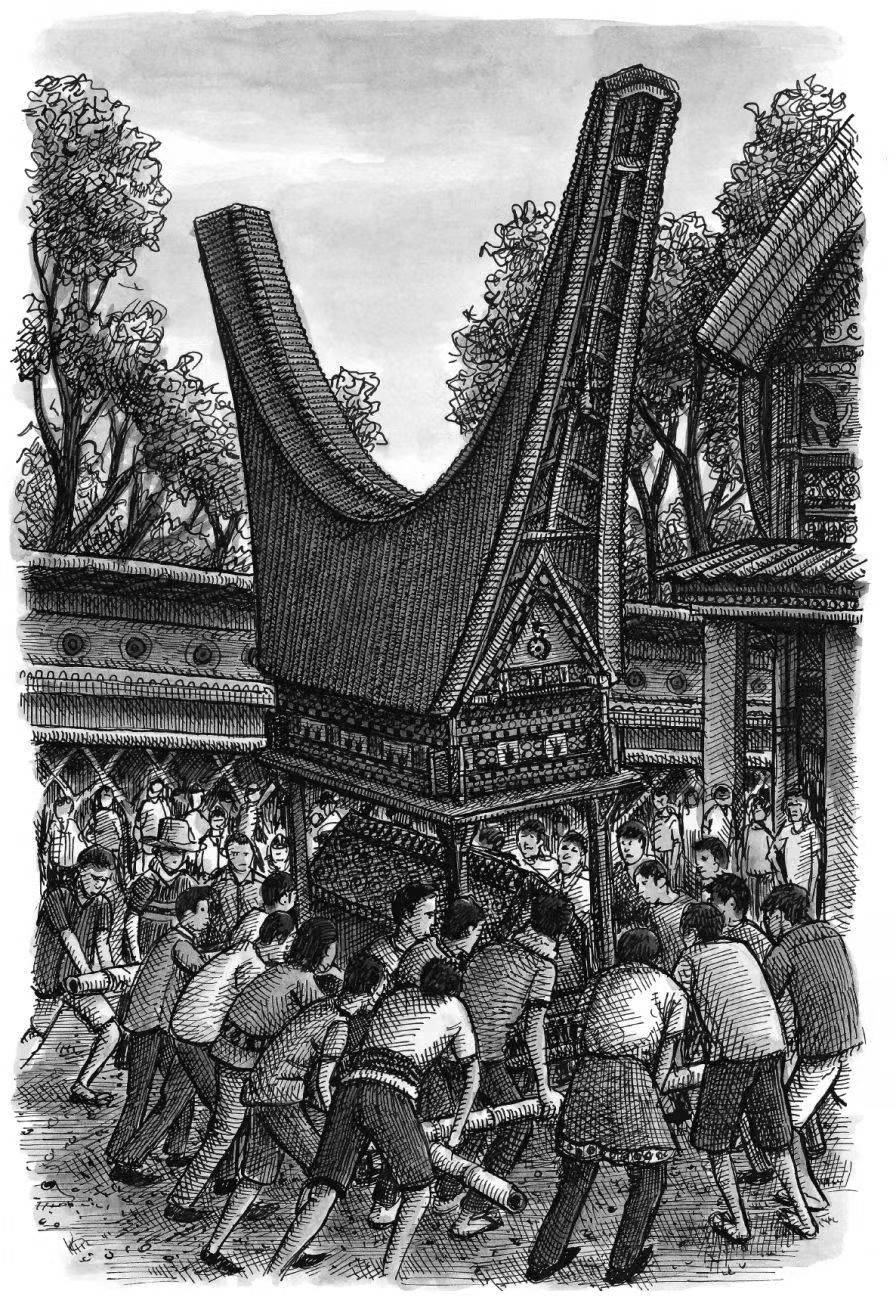
\includegraphics[width=\linewidth ,totalheight=0.95\textheight , keepaspectratio]{塔纳托拉雅的葬礼.jpg}
\caption{塔纳托拉雅的葬礼}
\label{fig:ta_na_tuo_la_ya_de_zang_li}
\end{figure}

人们一拥而入进了院子中央,而抬棺的队伍此时还在外面缓慢前进着。棺房比想象的要沉,小伙子们只能每走半分钟就把它放下来休息。

院子中央有一头强壮的水牛,它神情凝重,仿佛已经猜测到了自己的结局。它被一根短绳子拴在旁边的木桩上,可怜的模样...

游客(我猜的,他们有几个人皮肤白皙,带着西欧口音)统一集中在院子远处的角落里,所在之处和主场地隔着一排栅栏。这个措施反映出塔纳托拉雅死亡旅游业的一个棘手问题:如何才能既让游客近距离参观,又不让他们离得太近。我们也在这个“看台后排区”,但我不觉得有什么不妥。我找好地方坐下,保罗拿出相机准备拍照。为了让自己在闷热潮湿的天气里好过点儿,保罗今天换了一身行头:一件牛仔上衣、一条牛仔工装裤、一个警长徽章、一双波点短袜和一顶牛仔帽。

有些游客不太明白“后排区”的意义。一对夫妇直接坐进了留给死者家属的贵宾区。但当地人太客气了,没好意思把他们赶走。一个染着扎眼金发的德国老太太径直走到院子中央,用iPad对着小孩的脸就是一顿猛拍,还一支接一支地抽着红色万宝路烟。我真想找根拐杖钩着她的脖子把她弄走。

塔纳托拉雅的旅游业在最近几十年才兴起,20世纪70年代之前几乎没有人听说过这个地方。当时,印度尼西亚政府重点开发巴厘岛和爪哇岛的旅游业(事实证明他们做得很成功),忽视了塔纳托拉雅的独到之处——观赏性和仪式性兼具的传统葬礼。塔纳托拉雅不想再被其他印度尼西亚人看作“割取别人首级进行黑巫术”的地方,而是希望以保存良好的传统文化而闻名。

遗体终于被抬进了院子。抬棺人将棺房举起再放下,如此反复,口中哼着歌谣。他们一刻不停,直到全身的力气用尽之后才把棺房放到地上。他们喘了几口粗气,接着又把棺房扛在肩上,重复之前的动作。这种力量的交替让我看得入迷,西式葬礼的抬棺仪式一下子就显得有些古板。

这具遗体生前属于罗文纳斯·林汀。他是一位政府公职人员,也是一个农民,是村里的重要人物。我身后就放着一张5英尺高的照片,上面是林汀先生的脸部特写。照片里的人大概60岁,留着细长胡须,穿着时髦的蓝色西装。

身穿特色串珠服饰的小孩子在院子里追逐打闹,不时给搬运活猪的人让路。这些猪绑在竹板上,不断地发出尖锐的叫声。几个人把猪抬到屋后宾客看不见的地方。主屋的大门前挂着一个门帘,上面画满了迪士尼公主。在贝儿公主、爱丽儿公主和爱洛公主的注视下,这些猪穿过了通向屠宰场的大门。不知道我们早些时候碰见的黑毛猪是否也在其中。

塔纳托拉雅的葬礼可不是普通的自带酒水型(这里的“水”是水牛的“水”)活动。每一只献祭的动物都来自不同的人家,而且有记录可查。因为这套份子体系,人们通常不会错过别人的葬礼。就像阿古斯说的:“你在我妈妈的葬礼上送来一头猪,那我也要在你家举行葬礼时还一头。”看来,塔纳托拉雅式葬礼和美国葬礼一样,也存在过度花费的问题,因为不愿意被人看作不尊重死者。

到目前为止,这场葬礼上的仪式看上去都很繁复\footnote{繁多复杂。},但阿古斯说这已经比从前简单多了。阿古斯的父母从出生起就信奉阿鲁克教,但父亲在16岁时皈依了天主教。对此,阿古斯的解释是:“阿鲁克教里有7777种仪式,这太复杂了,人们只好改信别的。”我可不觉得天主教的仪式少,但就这样吧。

当牧师走到麦克风前开始布道时,人们安静下来。我听不懂他在讲什么,但能听出有几次他停下来,大声呼喊死者的名字向其致意:“罗——文纳斯,林——汀——!”他连续不停地讲了20多分钟,内容大多是重复的。很多人都准备离场,这时他贴近麦克风大吼了一声:“CO——E——!”那个动静活像是死亡金属乐队的主唱发出来的。告诉你,如果你恰好坐在音箱边上,却没在“CO——E——!”这个词出现时及时逃开,后果一定惨不忍睹。阿古斯告诉我,“COE”类似“好好听着”。据说,塔纳托拉雅的葬礼悼词在近几年深受电视节目的影响(舞蹈风格和服装设计也是)。

按照西方医学对死亡的定义,罗文纳斯于5月底去世,也就是葬礼前3个月。但按照塔纳托拉雅的习俗,他其实还活着。虽然已经没有了呼吸,但塔纳托拉雅人认为他只是处于类似发烧这样的生病状态。这个状态会一直持续到人们献上第一个活祭,通常是一头水牛或一头猪。献祭之后,罗文纳斯就可以ma’karu’dusan(咽下最后一口气),和作为祭品的动物一起死去。

人类学家迪米特里·辛吉罗尼斯在塔纳托拉雅进行了两年的田野研究,其间和一位名叫奈拉雅的当地老人建立了深厚的友谊,老人把迪米特里看作亲儿子一般。9年之后,迪米特里重返塔纳托拉雅,本以为能给奈拉雅一个惊喜,没想到她已经在两周前去世了。迪米特里来到奈拉雅家,她的一个亲戚把他领到后屋,然后告诉奈拉雅,迪米特里“回来了”。

\begin{quotation}
我端详着她的脸,然后盘腿坐下,在她耳边轻声问好。虽然一侧脸有腐烂、脱落的迹象,但她看上去十分宁静、安详……她只是“睡着”(mamma’)了,但她“知道”(natandai)我来看她了。不仅如此,她听得到也看得见我。她没有“死”(mate),只是“生病”(hot)了。因此,她还是“能够感受到一切”(nasa’dinganapa-apa)。
\end{quotation}

按照塔纳托拉雅的习俗,遗体在葬礼之前要放在家中。这听上去好像没那么震撼,但让我告诉你,在家中这段时间少则几个月,多则好几年。在此期间,死者的家人负责把遗体制成木乃伊,还要给他送饭、换洗衣物,时不时还要跟他说说话。

保罗第一次来塔纳托拉雅时,问阿古斯是否觉得家里待着一个已经死掉的亲戚很恐怖。阿古斯听了后放声大笑:“我小时候,我爷爷的遗体在我家待了7年。我跟我哥哥,我俩和他睡在同一张床上。每天早上,我们都给爷爷穿好衣服,然后把他靠墙立着,晚上睡觉时再把他放回床上。”

根据自己的所见所闻,保罗认为在塔纳托拉雅,死亡并不是一道强行把生者和死者隔开的“难以逾越的鸿沟”,而是一个模糊的界限。塔纳托拉雅人万物有灵的信仰也强调人类和非人类,不管是动物、高山还是尸体,两者之间都没有绝对的隔阂。

牧师总算讲完了,最后一嗓子“好好听着”也逐渐从音箱中消失。保罗轻轻走到我身边,低声说:“他们杀死那头牛后,应该顺手把某些游客也解决了。”

这时,两名男子好像收到信号一般,同时向院子里的水牛走去。一个人把一根蓝色的绳子从牛的鼻环中穿过。他的动作很轻柔,一边操作,一边用手挠着牛的下巴。水牛貌似没有意识到自己成了全场的焦点。另一个人蹲下来,把它的两只前蹄拴在地上的木桩上。

我不确定自己还在等待什么,也许是一段吟唱,也许是死者家属的相聚?这时,第一个人牵起牛头,从腰带里抽出一把砍刀瞬间割开了牛的喉咙,整个过程只有几秒钟。水牛向后仰起身躯,健壮的肌肉和牛角清晰可见。它想逃跑,却被绳子牢牢地固定在原地。一道鲜红的刀口出现在它的喉咙上,但没有血流出来,看来刀口不深。

好几个人冲上前拽住牛鼻环上的绳子,但没能制服它。水牛又踢又踹,猛烈地摆动自己的身躯,喉咙上的伤口撕裂开来,暴露在众人面前,这个场面让人难以直视。一个人拿出砍刀,朝牛脖子再次砍了下去。这一次,鲜血瞬间喷溅出来。

水牛发疯似的腾空跳起,力量大到挣脱了绳子和木桩的束缚,跌跌撞撞地冲向右侧的人群。现场一片混乱,尖叫声此起彼伏。我用小型摄像机拍下的视频记录下来的全是沉重的呼吸声和踩踏地面的闷响。我周围挤满了慌张的人,推搡之中,我不小心割破了手。

当时,我确信会有人(很可能是我自己)死于水牛的报复行动。最后,司仪成功把牛抓回了院子中央。不久之后,水牛倒地死去,喉咙上的伤口汩汩地往外冒着血。人群中有人哭有人笑,两种截然不同的声音混合成一种缤纷的复调。刚才的惊心动魄向葬礼注入了一丝活力。

\begin{center}
* * *
\end{center}

阿古斯正在打电话,语气很激动。

“出什么事儿了?”我问保罗。

“我们得带头猪过去。”

“我们去哪儿找猪啊?”

“阿古斯说他可以帮忙。不带头猪过去不礼貌。”

阿古斯的车已经坐满了,里面有我、保罗、阿古斯、司机和阿托——一个搭顺风车去隔壁村庄的15岁少年。车上已经没地方放猪了。

阿古斯挂断电话,向我们宣布道:“明天,我的一个朋友会骑摩托车把猪送来。”

阿托一路上都在疯狂地发短信。和一群成年人挤在一辆车里,换作哪个青少年都会这样吧。阿托家将在马聂聂节上给他叔叔和曾祖父开棺,这两个人在阿托还没出生的时候就去世了,因此阿托只能和他们的遗体相逢。

我们到达了目的地。这是一个由多个独立小村庄组成的村镇,没有所谓的中心。大部分村民都以种植水稻为生,包括我们此行的东道主。他们几户人家住在传统的长屋里,一共七栋,中间是公共生活用的庭院。院子里,一群红冠大公鸡正被几只瘦骨嶙峋的狗追着跑,边跑边“喔喔”地叫,狗后面还跟着几个笑哈哈的小孩。女人们正在用细长的竹竿敲打刚收获的稻谷,动作一刻不停。

村子里陆陆续续来了不少人,他们开始帮忙清理房子状的墓室。村子现在共有十几个墓室,都在自家屋子附近。每个墓室的门上都挂着一把大锁,这在以前是没有的。这么做不是为了提防邻居,而是因为几年前有人从村里偷走一具干尸,卖给了兰特包的一个收藏家。后来,村民打听到了是哪个收藏家,又去人家那里把干尸偷了回来。

几个人正聚在一起讨论如何给墓室通风。两年前,村里安葬了一个名叫约翰·汉斯·塔皮的村民。现在,他的深色木质棺材翘开了一个角,一打开墓室的大门就能看见。塔皮的儿子担心墓室里的空气过于潮湿:“希望父亲没什么事。但愿他还是干燥的,没有腐烂。”

今年的马聂聂节对约翰·汉斯·塔皮可谓意义重大。他的儿子认为,父亲在两年前去世时,家里在物质方面做得不够好——当时家里穷,没有杀牛献祭。他对此一直耿耿于怀,坚信没有活祭的话,“父亲就不能转世再生了”。不过,这一切将在这周改变:献祭的水牛已经选好了,正拴在附近的空地上呢。

两个墓室已经打扫完毕。一个女人敞开墓室的门,拿着一大罐柠檬味清新剂往里喷。

路的尽头有一户人家刚刚宰完猪,正等着新教牧师前来给他们新建的、能装下六个家庭成员的墓室赐福。他们邀请我们共进晚餐。

切成块的猪肉盛放在竹盘里,正架在火上烧烤。猪是在炉子旁边杀掉的,现在我们就坐在干掉的猪血旁吃晚饭,几只苍蝇绕着我们飞来飞去。不远处的竹架上挂着几只猪蹄。一只小狗冲进来,叼起一块滴着血的猪下水\footnote{猪下水,也叫猪下货、猪杂、猪杂碎,一般指猪内脏,或部分其他器官。}就往外跑。“哎哟!”厨子冲小狗大叫了一声,但没有阻止它带走战利品。

一个女人递给我一片竹叶,上面放了一个热乎的粉色饭团。这时,有人把竹盘上的肉从火上取下来,一大堆肥肉烧得滋滋作响。吃到一半时,我把这盘肉拿到跟前仔细瞧了瞧:焦脆的脂肪表皮上,一个个毛囊清晰可见。这可是动物尸体上的一块肉啊,我突然反应过来,随即感到一阵厌恶。

我虽然在人类遗体上花了很多时间,但不熟悉动物尸体,不是包装在保鲜膜和塑料泡沫盒里的动物我就不认识。法国人类学家努艾莉·维亚莱斯的一篇关于法国食物体系的文章中有一段话,我觉得也适用于西方其他国家:“屠宰被认为应该是工业化的,即大型化、统一化。不能存在暴力(最好是无痛的),也不能被人看见(最好根本不存在)。这几点即使做不到也要做到。”

\begin{quote}
即使做不到也要做到。
\end{quote}

饭桌上有一位老奶奶,年龄大到眼睛里蒙上了一层白膜。她拿起一小撮米饭,看向屋外山谷的方向。她不怎么与坐在旁边的人交流,也许她已经说不动话了。阿古斯用沾满猪肉残渍的手指捅了我一下,然后悄声说道:“那个新墓穴应该就是给她准备的。”阿古斯在调侃她,但说的也算是事实。这位老奶奶很快就会踏上祖先走过的路,搬到她的新房子里,那个“没有火也没有炊烟的房子”。

夜里,我们的猪乘着摩托车到了。它一着地就钻进其中一栋木屋,狼吞虎咽地吃着泔水。它完全没有意识到,因为我和保罗,这里将成为它的葬身之地。

这天晚上,我们都住在长屋里。长屋从外面看上去很宽敞,但我们进屋爬上梯子后却惊讶地发现,楼上只有一个没窗户的单人间。好在房间的地板上已经铺好了被褥,我们躺下后很快就睡着了。后半夜时,我们才意识到这里不是单人间,墙壁上的木闩拆下后,推开就可以看到另外三间屋子。一整晚都有人蹑手蹑脚地在我们房间周围进进出出。

\begin{center}
* * *
\end{center}

第二天一早,一阵阵凄凉的铜锣声从路边传来,正式宣告马聂聂节拉开帷幕。

我见到的第一具木乃伊戴了一副20世纪80年代的飞行员墨镜,镜框还镶着金边。

“哎哟,”我心想,“这哥们儿跟我中学的代数老师一个风格。”

一个年轻人把这具干尸立起来,另一个人拿起剪刀,把他身上的蓝色上衣从领口一路向下剪开,直到露出内裤边缘。木乃伊的上身和双臂就这样暴露在空气中。这个人虽然已经死去八年,但遗体保存得非常完好,表面上没有肉眼可见的伤口或裂痕。跟他隔着两具棺材的哥们儿就没那么走运了:全身上下都皱巴巴的,只有一层薄薄的干皮勉强搭在骨头上,要不是裹了一条镶有金边的毯子,估计早就散架了。

刚才那具木乃伊被放在地上,头下垫了个枕头,身上只剩下平角短裤和飞行员墨镜。一张8英寸×10英寸的遗像照片摆在它身旁。照片上的他看上去一点儿也不像我的代数老师,人在八年间的变化还真大。

几个女人在他旁边跪下,一边轻抚他的脸颊,一边大声哭着呼唤他的名字。当哭喊声逐渐停下时,他的儿子手捧一套工具刷(就是五金店里卖的那种)走了过来,开始清洁遗体。他用刷子轻轻扫过父亲粗糙的皮肤,每一下都很利落,并且充满爱意。一只蟑螂从父亲的平角短裤里蹿了出来,但他好像并不在意,继续手里的动作。这种打理遗体的方式我还是第一次见。

10分钟前,阿古斯接到一个电话,对方说有一家人正在河边一处难以到达的墓室中给死者开棺。我们迅速沿着水稻田旁的土路朝那个方向跑去。路的尽头是一条棕黄色的泥沟,附近没有垫脚的石头,也没有桥。我们只好一边抱怨,一边从泥里蹚过去,其间我还摔了个屁股蹲儿。

到达目的地后,我们看到至少有40具遗体被抬了出来,在地上一字排开。有些遗体裹着颜色鲜艳的布料,有的放在狭长的木质棺材里,还有的用印满卡通图案——凯蒂猫、海绵宝宝,以及一大堆迪士尼卡通人物——的毯子包着。这家人在遗体间走来走去,商议要先给谁开棺。有些死者他们已经不记得是谁了,有的则是重点关照的对象,比如某人亲爱的丈夫或某家的宝贝女儿,他们的家人都迫不及待地想再见到他们。

一个母亲正在打开16岁儿子的棺材。最先露出来的是一双弯曲变形的小脚,然后是手,看上去保存良好。站在棺材两侧的人试着抬起男孩,他们动作轻柔,确保不会碰坏遗体。他们成功地把男孩立了起来。男孩的躯干完好无损,但头部已经白骨化了:牙齿清晰可见,浓密的黑发还连在头皮上。但他的母亲毫不介意,此刻正欣喜若狂地看着他。这份喜悦也许是一时的,也许她从来都是这样,但不管如何,现在她正握住他的手,轻抚着他的面庞。

附近有一个人在用刷子清洁父亲的遗体。父亲的脸被蜡染布料制成的裹尸布染成了粉红色。“他是个好人,”他说道,“他有八个儿女,但他从没打过我们。我很难过,但又很开心,因为我现在能照顾他了,就像他以前照顾我那样。”

塔纳托拉雅人会把自己接下来的动作讲给遗体听:“现在,我要把你从坟墓里移出来。”“抱歉只给你买了烟,我最近手头有点儿紧。”“现在,我要脱掉你的外衣。”“你女儿和女婿从望加锡过来看你了。”
我们在这个河边墓穴碰到了这家的族长,他对我们的到来和送上的香烟表示感谢。他允许保罗拍照,也同意我问问题,但条件是答应他的一个请求:“如果你们在村子里碰见外来人,不要告诉他们这个地方,这里是我们的秘密。”

我想起前几天葬礼上那个粗鲁的德国女人,一边抽烟,一边把iPad贴在别人脸上乱拍。我担心自己也变得跟她一样——我们渴望把期待已久的事物看个遍,但不承想这让我们变成了不受欢迎的人。

\begin{center}
* * *
\end{center}

我们穿过稻田返回主路,正好赶上东道主开棺打理自己家的遗体。我认出一个在兰特包当平面设计师的同龄人。昨天深夜,他骑摩托车赶了回来,在我们睡觉的房间钻进钻出。他指着一具包在金色布料里的骷髅说道:“这是我兄弟,17岁时骑摩托车出车祸死了。”然后指了指旁边的遗体,“那是我爷爷。”

我们下方的山坡上有一家人在野餐。用餐完毕后,他们把死去七年的祖父平放在方格桌布上。这是他祖父第二次参加马聂聂节,遗体状态极佳,看不出有任何损坏。这家人先用软刷清洁他的面部,再把他翻过来清理脑后干裂开的皮肉。拍摄全家福时,祖父被立在中间,家庭成员纷纷围过来,有的表情严肃,有的面带笑容。我正津津有味地看着,一个女人招呼我过去一起合影。我朝她摆摆手,意思是“还是不用了吧”,但他们坚持要叫上我。于是,一张奇特的合影出现在印度尼西亚的深山里,上面是我、一个塔纳托拉雅家庭和一具焕然一新的干尸。

我之前听说把遗体制成木乃伊通常发生在气候寒冷干燥的地区,没想到在湿润多雨的印度尼西亚也能这么做。那么问题来了:这里的遗体究竟是怎么变成干尸的呢?不同的人会给你不同的答案。有人说他们用的是自古流传下来的方法——把油灌入死者的嘴巴和喉咙里,再用特制的茶叶和树皮覆盖全身。茶叶的茶多酚和树皮将皮肤中的蛋白质收紧,从而强化了皮肤的柔韧性和硬度,这样就能够更有效地抵挡细菌入侵。这个过程与标本师对兽皮进行处理使之长久保存的过程类似(所以有一种皮革叫“植鞣皮”)。

塔纳托拉雅现在还流行一种新潮的干尸制作方式:把防腐师的好朋友福尔马林注射到遗体中。有一个女人告诉我她无法接受这种方式,因为不愿意死去的家人被针扎。“但我知道有人这么做。”她压低声音说,好像发现了什么见不得人的事。

生活在塔纳托拉雅这部分的村民可以称得上业余人体标本师了。既然他们现在和北美人民都用同一种化学制剂给尸体防腐,我不明白为什么西方人依然会被他们的习俗吓个半死。原因应该和尸体干燥的程度无关,而在于塔纳托拉雅人不把遗体密封在棺材里,也不把棺材搁置在水泥做成的地下墓穴里,而是大大方方地让遗体和活人待在一起。

昨天,我碰到了约翰·汉斯·塔皮的儿子,今天我要去见约翰·汉斯·塔皮本人。他被平放在地上晒太阳,身上只穿了一条平角裤,手腕上戴了一块金表。他的胸腔和腹腔注满了福尔马林,因此这两处保存得异常完好。相比之下,他的面孔已经变成黑色,上面布满了斑点,白色的骨骼依稀可见。这时,他的家人把刷子伸到他的平角裤里,开始清洁他那干瘪的阴茎。不出意料,家人的脸上写满了尴尬。他们互相开了个玩笑,然后继续手里的活儿。

小孩子们在木乃伊之间跑来跑去,他们有时会在某具遗体面前突然停下,仔细瞧一瞧之后再伸手捅一下,然后大叫着跑开。一个5岁的女孩爬了上来,和我一起坐在一个墓室的屋顶上看着他们玩闹。我俩没有说话,心照不宣地享受着俯视他人的奇妙快感。

阿古斯发现我在屋顶上,向我喊道:“喂,我在想我之后是不是也会变成这样。肯定会的,是吧?”

我们回到留宿的那栋房屋后,一个4岁的男孩过来偷看我们吃饭。他从篱笆后面探出头,每次我回头冲他做鬼脸时,他都开心地大叫。这时,他妈妈过来告诉他不要打扰我们,于是他给自己找了个小刷子。他穿过院子走到一堆干竹叶旁坐下,用刷子全神贯注地在地上刷来刷去,保证每一条小裂缝都被刷到。如果马聂聂节一直存在,长大成人的他也一定会去清洁某具遗体,遗体的主人说不定就是我们这次碰见的某个村里人。

\begin{center}
* * *
\end{center}

第二天清晨,约翰·汉斯·塔皮已经换上了一套新衣服...。他今天要被搬去路尽头的一间新墓室里,墓室的墙壁是浅蓝色的,屋顶上立着一个白色十字架。里面的装饰走的是多元文化路线:除了传统的水牛符号之外,还有玛利亚之心、耶稣祈祷像以及《最后的晚餐》全景图。

家里人把约翰立起来,跟穿着新衣的他拍了最后一张合影,便把他放回棺材。他们把闪亮的黑皮鞋从他脚上脱下放在旁边,给他裹好毯子,随后合上了棺材盖。棺材两侧被擦拭干净之后,他们就把棺材扛在肩上出发了。鼓声和诵经的声音伴随了他们一路。

我往车上装东西时,阿古斯走了过来。“知道吗,现在就有具尸体在这栋房子里。”他指着跟我们木屋只隔了10英尺的一栋传统房屋说道。一位名叫山达的70岁老太太两周前死在这栋房子里。这家人一直瞒着我们,就是想看看我们知道后会有什么反应。

“你想见见她吗?”阿古斯问道。

我慢慢地点了点头。不知为什么,我觉得我们应该就睡在尸体隔壁。

“嘿,保罗,”我叫醒正在屋里补觉的保罗,“跟我下楼,给你看样东西。”

在阿古斯的指导下,我们给山达带来了一些吃剩的食物——她应该知道是我们送的。我们钻进里屋,看到山达躺在一张竹席上,身上盖着一条绿色的格纹毯子。她穿着一件橘色的衬衫,脖子上围了一条粉色的围巾,身边还放着钱包和食物。她的脸上围着一块布,面部皮肤有着橡胶般的质感,这在防腐后的遗体上很常见。

山达是由一个本地的专业人员用福尔马林防腐的。她的家人没有亲自操作,因为觉得福尔马林太“辣眼睛”。山达一家子都是成功的稻农,没有时间按照传统天天照料她的遗体。

她会在家里一直住到搬进墓室。这期间,家人给她端茶倒水,她在梦里与家人相会。距离她穿过生与死那条模糊的界限只有两周,因此家里人决定,等味道散去后就跟她一起睡。

阿古斯小时候跟他祖父的遗体睡了七年。他耸了耸肩,说道:“这种事情我们已经习惯了,这就是生与死。”

\begin{center}
* * *
\end{center}

在前往印度尼西亚之前,我试图在网上查询与塔纳托拉雅有关的信息,想先看看会有什么样的丧葬仪式在等着我。搜索出来的信息很少,起码没什么英语的。

照片也没有几张,其中最清晰的一张来自英国报纸《每日邮报》。我不知道他们是从哪儿得到的这张照片,因为他们显然没有派记者去。页面上的评论区很有意思,一条评论写道:“天哪,他们对这些逝者做了些什么呀?”另一条评论则写着:“讲真,这是对死者的大不敬。”

确实,如果说把莎莉姨妈从明尼苏达的坟里挖出来,把她放到高尔夫球车上在郊区民宅附近转一圈儿,那么是的,这的确是对死者的大不敬。但这些心智不健全的网友没有意识到,人死后,亲情还会继续存在。塔纳托拉雅人不但不觉得开棺掘尸是对死者的不尊重(事实上,这是对死者最大的尊重),而且认为这是与逝去的家人维持情感的一种方式。

作为一名殡仪业者,我总会碰到各种各样关于母亲遗体的问题。你不知道我听到了多少次:“我妈妈11年前在纽约州北部去世,防腐后葬在我们的家庭墓地里,你能告诉我她现在变成什么样了吗?”这个问题的答案取决于多个因素:天气、土壤、棺材、化学品。所以,我给不出一个完美答案。当我看到塔纳托拉雅人与母亲的遗体互动时,我意识到他们不需要通过殡仪人员了解遗体的状况。他们很清楚自己的母亲死后是什么样子,哪怕她已经死了11年。相较于与死去的母亲重逢,还是人类的胡思乱想更可怕一些。


\hr 

\section{墨西哥的米却肯州}
\hr
一具头戴黑色圆顶高帽、嘴里叼着雪茄的骷髅疯狂地挥舞着细长的双臂,朝华雷斯大街俯冲下来。这个庞然大物高达15英尺,在黑压压的人群中显得极为壮观。一群打扮成卡特里娜骷髅的男人和女人跟在它身后,一边欢呼雀跃,一边舞蹈。华丽优雅的卡特里娜骷髅是这里的标志性形象。当身着阿兹特克勇士戏服的旱冰方阵表演旋转时,一大片金色亮片从礼花炮中射出,街上的几万名观众顿时爆发出热烈的欢呼。

如果你看过2016年的詹姆斯·邦德电影《007:幽灵党》,就会认出这充满了鲜花、骷髅、魔鬼和大型卡通气球的狂欢,正是墨西哥城一年一度的亡灵节大游行。这部电影的片头,就是西装革履的邦德戴着骷髅面具穿过嘈杂的人群,与一名同样戴着面具的女子溜进了旅馆。

不过请注意,这部邦德电影并没有从亡灵节大游行中获取灵感,亡灵节大游行反倒是因为这部电影才存在的。墨西哥政府担心世界各地的人们观看完影片之后,会来墨西哥参加其实并不存在的游行,于是现招募了1200名志愿者,用一年的时间打造出这场四个小时的盛会。

亡灵节为每年11月的头两天。在这两天里,死去的人会重返人间,与活人一同享受人间的乐趣。在有些人看来,这个愚蠢的游行把本应以家庭为中心的、私人化的节日庆祝商业化了。另外一些人认为,这恰好代表了亡灵节正在向更加世俗的全国性节日演变,在全球的瞩目下毫不畏惧地展现墨西哥的历史文化。

游行结束后,我们艰难地走在装饰亮片成堆的街道上。跟我同行的是莎拉·查维斯,她是我建立的非营利组织“死亡新秩序”的总监。她发现这里到处都有亡灵节的装饰品,不管是在家里还是在商店,卡特里娜骷髅和鲜艳的骷髅剪纸随处可见。

“噢!”听起来她好像突然想起一件重要的事,“忘了告诉你,我们酒店旁边的星巴克在卖亡灵面包。”亡灵面包就是一种撒满糖霜的、带有立体骷髅造型元素的圆面包。

明天,我们就要动身前往西部的米却肯州。那是比较偏远的地区,当地人有着漫长的庆祝亡灵节的传统。但是在墨西哥,亡灵节在20世纪的一段时间里并没有受到普遍欢迎。到了20世纪50年代,墨西哥的城镇居民仍然把亡灵节视作老掉牙的民俗节日,认为只有文明社会里的边缘人才会庆祝这种节日。

这种情况不久之后就迎来了反转,主要原因之一就是万圣节从美国南部传入了墨西哥。在20世纪70年代早期,用记者玛利亚·路易莎·门多萨在她的文章中的话来说,万圣节习俗的核心就是“光彩夺目的聚会”。“黑猫、南瓜和戴着尖顶帽坐在扫帚上的女巫如果只是出现在侦探小说里,我倒觉得还好,因为这些东西跟我们的文化一点儿关系都没有。”门多萨继续写着,“普通的墨西哥人忽视了那些乞讨要饭、靠擦车窗讨生活的孩子。在富人区,我们的中产阶级模仿美国得州人,让孩子们穿上可笑的服装去别人家里要施舍。要知道,这些孩子从未空手而归。”

学者克劳迪奥·龙尼茨对这一时期是这样描述的:亡灵节“变成了国家形象的统一代表”,站在了“美式万圣节狂欢”的“对立面”。那些曾经抗拒亡灵节(或者生活在从不庆祝亡灵节的地区)的人逐渐把庆祝亡灵节视作墨西哥的传统。亡灵节不仅回归了主流城市(瞧瞧那个邦德引发的大型游行),还成为丧失权利的弱势群体的发声通道。他们在亡灵节上悼念那些远离公众视野的人,包括性工作者、本土性少数人权倡议团体和死在美墨边境线上的同胞。在过去的40年间,亡灵节成为整个墨西哥的流行文化、旅游文化和反抗文化的代名词。墨西哥本身也因成功地打造了全民参与的祭奠文化而走在世界前列。

“我小时候,跟我一起生活的长辈都是一些自我厌恶的墨西哥人。”莎拉说道,此时我们正坐在米乔坎的酒店房间里,“他们生活的环境告诉他们,他们没什么可自豪的,他们应该对自己的一切感到羞愧。他们应该融入。要想在美国获得快乐,就得变得和白人一样。”

20世纪初期,莎拉的祖父母从墨西哥蒙特雷搬到东洛杉矶的查维斯山谷区定居。20世纪50年代,政府通过公函告知该地区的近2000个家庭——大多都是低收入的墨西哥裔美国农民——他们必须卖掉自己的房产,给政府的公共住房项目腾地方。政府保证,在项目完成后,不仅会在原地新建学校和操场,还会优先给予搬迁居民回迁的机会。这些家庭只好搬走,原先的社区也被拆毁。然而,洛杉矶政府取消了公共住房项目,转而与纽约的商人共同兴建道奇体育场。包括罗纳德·威尔逊·里根在内的体育场项目支持者公然把反对者称为“痛恨棒球的家伙”。

由于一项歧视性的住房政策,从查维斯山谷区搬离的墨西哥裔美国人被赶到洛杉矶东部。在搬迁的过程中,莎拉的父母步入成年,二人在19岁的时候生下了她。

“直到今天,我的奶奶、姑姑和叔伯一谈到查维斯山谷区,还是会伤心得不得了。他们特别、特别想念那个地方。”

莎拉出生后,她的家人不允许她学西班牙语。她的浅色肌肤让她成为家里最受宠爱的孙辈。她墨西哥人的一面只能留在家里。在洛杉矶长大的莎拉,不停地游走在与她关系疏远的母亲、在好莱坞从事服装道具营生的父亲(时至今日,他都认为自己是“美国原住民”,而不是墨西哥人)和祖父母之间。莎拉只当自己是个碰巧带有墨西哥血统的美国人,家里的墨西哥文化氛围和自己的关系不大。

2013年,莎拉已经在学前班和幼儿园当了10年的老师。她与自己工作上的搭档鲁本坠入爱河,不久后,两个人决定是时候要个孩子了。莎拉很快就怀孕了。对她来说,有了这个孩子就意味着“一个真正的家庭,我的家庭,一个天选之家,没有谁能从我手里夺走”。

可惜事与愿违,莎拉的儿子在六个月大的时候胎死腹中。在接下来的日子里,莎拉心里“放不下任何人、任何事”。她与父母渐行渐远,觉得自己孤独极了。有那么几天,她甚至想消失在房屋后面的橙树林里。她不停地自责:是不是我搬东西的姿势不正确?我是不是吃了不该吃的东西?“女人的本质是带来生命之人,”莎拉说道,“我的身体却是一个坟墓。”

她觉得对朋友和同事来说,自己就是一个行走的辐射源。她知道,在人们理想中的世界里,孩子是可爱的,不会受到伤害。“这个社会要求我藏起悲伤,”她继续说道,“人们不想面对这种恐惧,而我恰好就成了这种恐惧的代言人。我是一个恶魔。”

莎拉在网上搜遍了那些遭受丧子之痛的母亲的故事。她找到了几个好心人建立的网站,但它们都带有一些基督教的意味(例如,“我的天使躺在上帝的臂弯中”),里面的故事也是老生常谈,一直在绕弯子。在她看来,这些看上去很美的话不过是一堆空洞的陈词滥调,无法捕捉到她的悲痛和渴望。

在寻找安慰的过程中,她将目光转向了自己的文化与传统。“莎拉,你是墨西哥人,你来自无疑是这个世界上与死亡关系最紧密的文化。”她想,“你的祖先会如何处理这种悲剧呢?”
\begin{center}
* * *
\end{center}
墨西哥诗人奥克塔维奥·帕斯有一段著名言论。他说,当纽约、巴黎、伦敦等西方城市的居民还在担心频繁提起“死亡”这个词会让自己“咬到嘴巴”时,“墨西哥人已经无时无刻不在谈论它、嘲讽它、爱怜它、取悦它,甚至与它同眠。死亡是墨西哥人最喜欢的玩乐之一,也是他们永恒的挚爱”。

不过,这并不意味着墨西哥人不惧怕死亡。他们与死亡的联结源自长达几个世纪的暴行,可谓来之不易。“墨西哥没有成为一个令人骄傲并强大的帝国,”克劳迪奥·龙尼茨解释道,“这个国家不断被列强和独裁者欺压、侵略、占领、分裂、敲诈。到了20世纪,当西方世界对墨西哥的镇压和对死亡的抗拒双双达到顶峰时,墨西哥与死亡之间愉快、亲密的联系逐渐成为国家形象的奠基石。”

对莎拉而言,接受儿子的死不等于抹杀对死亡的恐惧,她知道自己不可能不惧怕这必然的命运。她只是想适应死亡,只是想开诚布公地谈论死亡。就像帕斯说的,时刻“谈论它、嘲讽它、爱怜它”。

许多来自移民家庭的孩子发现自己越发远离家族所传承的文化传统,就像莎拉经历的那样。臭名昭著的美国殡葬体系通过立法和出台管理条例,大肆干预多元化的丧葬习俗并强制其与美式规范同化。

莎拉最初是通过画家弗里达·卡罗的作品与墨西哥文化建立起联系的。弗里达·卡罗是墨西哥的“痛苦的女主人”,对莎拉的影响最为深远。在1932年的画作《墨西哥和美国边境线上的自画像》中,卡罗站在假想出的墨西哥和底特律的边境上,脸上充满了蔑视。那时,她和作为壁画画家的丈夫迭戈·里维拉正在底特律生活。边境线上的墨西哥一侧画满了骨头、废墟、植物、花朵和深深植入土壤中的粗壮的根茎,底特律一侧则是工厂、摩天大楼和滚滚浓烟——一个掩盖了大自然生死循环的工业城市。

在底特律生活时,卡罗怀孕了。她把这个消息写信告诉给了自己的前任医师利奥·埃劳塞,他们二人在1932年到1951年一直密切通信。她担心这次怀孕有很大的风险,因为在那次电车事故中,她的部分骨盆粉碎性骨折,子宫也被刺穿。卡罗在信中写道,底特律的医生“给我开了打胎用的奎宁和高浓度蓖麻油”。但这些化学药品没能终止妊娠,医生也拒绝为她进行堕胎手术。卡罗很有可能要冒着生命危险分娩。她请求埃劳塞给那名底特律医生写信:“堕胎是违法的,他应该是害怕做违法的事。但再这样拖下去,恐怕会错过手术的最佳时机。”我们不知道埃劳塞有没有按照卡罗说的做,但两个月之后,她遭遇了严重的流产。

卡罗以这次经历为灵感创作了《底特律的流产》。画里的她赤裸着躺在医院的病床上,鲜血染红了床单。几个物体飘浮在她的周围,分别是男胎(她的儿子)、手术工具以及具有象征意义的蜗牛和兰花,均由红色丝带做成的脐带连在她的肚子上。底特律了无生气的工业建筑构成了天际线,突兀地矗立在画面后方。艺术史学家维克多·萨穆迪奥·泰勒称,除了表达对底特律发自肺腑的憎恶,哀诉发生在自己身上的可怕不幸,“这幅画作是卡罗第一次有意识地画出自己的故事,画出自己最隐秘、最痛苦的内心”。

莎拉一直淹没在“上帝对你早有计划”这种空洞的说辞中,卡罗的画作和书信里的直白表达对她来说无疑是一种安慰。她在卡罗的身上,看到了另一个因为孩子、身体而被迫与命运的无常进行抗争的墨西哥女人。卡罗用画笔展现出这种痛苦和困惑,毫不羞耻地描绘自己的身体和哀痛。

莎拉的儿子死于2013年7月。同年11月,她和自己的伴侣——同样是墨裔美国人的鲁本在亡灵节时来到墨西哥。“我们不是游客,不是来看‘死亡’的。”莎拉说道,“我们每天都与死亡在一起。”

穿行在精致的祭坛和骷髅装饰品之间,莎拉感受到了在加利福尼亚州从未体会过的冲击与平和。“来到墨西哥后,我发现这是一个能让我放下悲伤的地方。这里认可我的悲伤,我不再是那个让别人不舒服的人。我终于可以喘口气了。”

莎拉和鲁本来到了以收藏木乃伊而闻名的瓜纳华托。19世纪末,当地人要给葬在坟场的死者缴一笔“坟墓税”来获得“永久”埋葬的资格。如果死者的家人交不起这笔钱,那么死者的遗体就会被挖出来给刚死的人腾地方。在一次例行的挖掘作业中,工作人员惊讶地发现挖出来的不是白骨,而是一具具“表情狰狞、形状怪异的干尸”。原来,土壤中的化学物质在当地的气候条件下能够天然地将遗体木乃伊化。

瓜纳华托市政府在接下来的60年里,不断地挖出了木乃伊。轻度干尸化的遗体被直接火化,完全呈木乃伊形态的则作为展品收藏在木乃伊博物馆。

20世纪70年代,作家雷·布拉德伯里到访该博物馆,并以陈列在里面的木乃伊为灵感创作了一个故事。他之后写道:“这个博物馆让我的心灵饱受创伤。我害怕极了,只想赶紧逃离墨西哥。我接连做噩梦,梦见自己死后被当作展品,和一屋子被金属丝线固定的干尸关在一起。”

由于这些木乃伊是天然形成的,不是出于防腐的目的刻意而为之,因此他们都大张着嘴巴,手臂和脖子呈扭曲状。人死后,遗体会重新回到“肌肉松弛的状态”,放松的下颌导致嘴巴张开,眼睑失去张力,四肢的关节也变得极度松垮。总之一句话,遗体不会自己使劲,它们不再按照活人的规矩来。瓜纳华托木乃伊的吓人形态不是为了“吓唬”布拉德伯里先生而人为制作的,那只是人死后正常的生理变化现象而已。

这些木乃伊现在还在展出。莎拉一点儿也不觉得它们可怕,她走到一个黑暗的角落,在一个身穿白色连衣裙、躺在天鹅绒垫子上的木乃伊女童跟前停下。“她看上去像一个被光芒围绕的天使,那一刻,我觉得自己可以永远站在那里看着她。”

莎拉默默地流着眼泪,一个女人看到后递给她一张纸巾,然后轻轻地拥抱了她一下。

博物馆里其他的木乃伊儿童也有自己的专属道具,比如拿着权杖和戴着王冠的Angelitos(“小天使”)。在20世纪早期的墨西哥以及其他拉丁美洲国家,人们把死去的婴儿和小孩视作能与上帝沟通的神体,类似于圣徒。这些“小天使”已经不再背负原罪,能够给尚在人间的家人带来恩惠。孩子的教母负责打理遗体,她把遗体清洗干净,然后给遗体穿上小号的圣徒服装,再把蜡烛和鲜花摆在遗体周围。孩子的母亲在这个过程结束之后才能见到遗体。此时,呈现在她眼前的是一个不再带有世间忧伤的天人,已经准备好回到上帝身边了。

孩子的家人会邀请朋友和亲属参加葬礼聚会。这么做不仅是为了缅怀死去的孩子,也是为了给这个孩子留下好印象以获取恩惠——别忘了,这个孩子现在已经拥有了灵力。有时候,人们甚至会带着孩子的遗体参加一个又一个聚会,遗体由同龄的小朋友抬着,后面跟着父母和亲属。“小天使”通常会出现在拥有恢宏场景的照片或画作中。

虽然莎拉不相信圣徒和来世,但是这种文化承认孩童的死亡,这一点深深地打动了她。“他们对待这些孩子的方式太特别了,很多事就是专门为这些孩子做的。”她说道。不管是聚会、作画,还是游戏,这里的人们为死去的孩子做了很多,而不是沉溺在孤独和无尽的缄默中。
\begin{center}
* * *
\end{center}
每年11月1日的夜晚,生与死的界限变得薄弱而模糊,死者轻易就能跨越这道坎儿。在米却肯州的小城圣达菲拉古娜,一群上了年纪的妇女正端着亡灵面包和水果,拜访那些在今年失去亲人的邻居,铺满鹅卵石的小道上到处都是她们走家串户的身影。

我低头钻过画有金盏花的门帘进到玄关。大门正上方挂着一个相框,里面是赫尔海的照片。赫尔海死的时候才26岁。照片上的他反戴一顶棒球帽,身后贴着好几张乐队的海报。“活结乐队?这个我可不好评价,赫尔海。”我琢磨着,同时在思考对一个死人的音乐喜好评头论足是不是不太妥当。“噢噢,那是错配乐队!算你有眼光。”

穿过玄关就是赫尔海的祭坛,一共三层。里面每一个祭品都是他的家人和朋友送来做诱饵的——诱使他在这一晚回家。赫尔海在今年身亡,因此他的家人先在家中设立祭坛,之后再把祭品带去他的坟墓。只要他的家人经常去扫墓,邀请他与生者重逢,他就每年都能回家看看。

祭坛的最下方有一个黑色的高脚杯,里面放着柯巴脂香料,辛辣的气味在空气中飘荡着。水果和面包足足堆了3英尺高,旁边放满了装饰用的蜡烛和金盏花。这一晚,随着越来越多的街坊邻居过来送上自己的那一份祭品,这个祭品台只会变得越来越高。重返人间并不意味着赫尔海要变成一具活跳尸,他会以灵魂的形态回到家中,用灵体特有的方式吃掉那些水果和面包。

摆在祭坛正中间的是赫尔海最爱的白色T恤,上面印着一个表情悲伤的小丑和手写体的“小丑”字样。等待他回家的还有一罐可乐(可乐的魅力我太了解了——这听起来也许有些不着调,但如果家里有一瓶健怡可乐等着我,我也会起死回生的)。T恤的上方挂着一些传统的基督教饰品,我看到了几个圣母玛利亚和一个钉在十字架上的血淋淋的耶稣。天花板上悬挂着色彩缤纷的剪纸,形状是脚踩自行车的骷髅。
祭坛旁边围了十几个人,他们都是赫尔海的家人,正在为迎接客人做准备。他们今晚很有可能要忙活到深夜。几个身穿闪亮公主裙的小家伙跑来跑去,脸上画着卡特里娜骷髅花纹,手里还拿着挖空内瓤的小南瓜,用来装大人给的糖果。

莎拉早就买好了满满一袋糖果。消息不胫而走,一大帮脸上画有骷髅彩绘的小孩提着点了蜡烛的南瓜灯把她团团围住。“女士,女士,谢谢你!”莎拉顺势蹲下,带着幼儿园老师特有的沉着和爱意给他们发糖。“我以前也在亡灵节的时候给班里的小孩做南瓜灯,里面也有蜡烛,跟他们现在手上拿的一模一样。可惜一点儿火光就能让管理部门把活动叫停。”她苦笑了一下。

圣达菲拉古娜是布雷佩查人的故乡,这一原住民以建造造型独特的金字塔和制作用蜂鸟羽毛制成的装饰画而闻名。1525年,布雷佩查人正因天花肆虐而变得脆弱不堪。当听闻勇猛善战的阿兹特克人已成为西班牙人的手下败将时,布雷佩查的领袖只好宣誓效忠西班牙。时至今日,这个区域的学校依旧在实行布雷佩查语和西班牙语双语教学。

许多现在流行的葬礼仪式元素,例如音乐、熏香、花朵和食物,布雷佩查人早在16世纪西班牙入侵之前就使用了。到了西班牙殖民时代,根据一名多米尼加男修士的记载,布雷佩查人很乐意接纳天主教的万圣节和万灵节,因为这跟他们已有的纪念亡者的节日完美契合。

在接下来的几个世纪里,殖民者想方设法地根除原住民祭奠死者的习俗,因为这“吓坏了杰出的精英阶层,他们竭尽全力要把死亡从社会生活中赶走”。1766年,皇家罪案处禁止原住民进行扫墓活动,强行切断了他们与死者的联结。不过,原住民总能找到钻空子的方法,这个习俗也就保留下来了。

我们来到另一户圣达菲拉古娜人家,只见门口的牌子上用布雷佩查语写着“欢迎回家,柯奈李奥神父”。柯奈李奥神父的祭坛占满了一整间屋子。我把橘子和香蕉摞在水果堆的最上方。这时,这个家族里几个年长的妇女围过来,给我们递上一大碗还冒着蒸汽的猪肉炒番茄和几杯玉米粥——一种用玉米、肉桂和巧克力做成的热饮。对死者家属而言,这一晚不能单方面地接受别人送来的慰问品,邻里间的这种交流是相互的,他们也要有所给予。

坐在屋子一角观察我们的正是柯奈李奥神父本人——其实这是一具真人大小的塑像。柯奈李奥神父坐在折叠椅上,身披一件斗篷,脚蹬一双黑色的高帮靴子,头上的白色牛仔帽遮住了半张脸,一副正在睡午觉的样子。

祭坛的中间是一个相框,照片里的柯奈李奥神父也戴着一顶白色牛仔帽,和塑像头上的是同一顶。相框后方的墙上挂着一个木质十字架,再往上则挂着一串色彩鲜艳的骷髅头糖块和……面包圈。“莎拉,往祭坛上挂面包圈正常吗?”

“正常。”莎拉答道,“你之后会看见更多的面包圈。”

又拜访了几户人家之后,我问莎拉哪户人家的祭坛让她最受触动。“让我最开心的不是祭坛,而是和孩子们在一起的时候。”她边说边示意我看向旁边的一个小男孩,这个小孩三四岁的样子,身穿超人的服装,手里拿着用南瓜做成的小篮子,“那感觉又苦又甜。如果我的儿子还活着,他现在应该和那个孩子一样大了。”话音刚落,“小超人”就害羞地把篮子伸过来要糖。

\begin{center}
* * *
\end{center}

我们的墨西哥之旅还在继续。现在,我们一路向南前往辛祖坦小镇。亡灵节期间,这里会举办热闹非凡的街头文化节。小贩们用大大的金属锅煎着猪肉和牛肉,街边店铺门口的音响里传来震耳欲聋的音乐,孩子们在街上兴高采烈地放爆竹。镇子的边缘地带有一处小山丘,顺着斜坡走上去,就来到了镇里的公共墓地。

在11月1日这天夜游墓地,不愁没有启示性的收获。为了迎接死者回家,墓地里有成千上万支蜡烛在燃烧,都是人们用一年的时间积攒下来的。一个小男孩认真地把祖母坟墓上熄灭的蜡烛重新点燃或换上新的,小手在上百支蜡烛之间忙碌着。烛光混合着金盏花和熏香的香气,给一座座坟墓笼罩上一层金色的薄雾。

最近几年,许多美国城市也开始举办亡灵节庆祝活动,其中就包括在好莱坞永恒墓园举行的大型庆典。好莱坞永恒墓园距离我在洛杉矶的殡仪馆只有几分钟的车程,我已经参加过好几次了。那里举办的庆典规模宏大、执行到位,但情感上远不及辛祖坦。此时此刻,站在辛祖坦的墓地里,就像站在一颗光芒四射、怦怦直跳的心脏中间,充满了安全感。

...

莎拉站在1岁的马可·安东尼奥·巴里加的墓前。墓碑上的照片上,一只白鸽从马可的头顶飞过。马可的坟墓高达7英尺,简直像个堡垒。可以说,坟墓有多高,他的父母就有多悲伤。马可死于20年前,但蜡烛和鲜花依然堆满了他的坟墓,看来丧子之痛从未从他父母的心头散去。

我在来墨西哥之前就知道莎拉失去过一个孩子,但不清楚来龙去脉。我们俩在酒店房间说话时,莎拉向我倾诉了这场灾难背后的故事。

莎拉第一次做超声波检查时,一直和她拉家常的护士用探头在她肚子上扫了几下,随即陷入了沉默。“我去叫医生。”过了一会儿,护士说道。

第二次做超声波检查时,医生彻底惊呆了。“呃,这只脚是内翻足,”医生把看到的影像描述给莎拉,“这只手有三根手指,另一只手有四根。心脏发育不良。哦,再看看这个——他有两只眼睛!大多数这样的胎儿不会有两只眼睛。”最后,医生给了莎拉致命一击,“我认为这个孩子活不到你临盆的时候。”

莎拉的孩子患有13-三体综合征。这是一种罕见的染色体异常,会导致孩子智力发育不全和身体畸形。绝大部分患有此病的孩子熬不过出生后的头几天。

第二个医生直白地告诉莎拉:“如果你是我的妻子,我会建议你放弃这个孩子。”

第三个医生给了莎拉两个残酷的选择:第一个是在医院引产,引产之后,孩子只能在子宫外短暂地存活一段时间,然后死去;第二个是终止妊娠。“洛杉矶有一名医生可以帮你。”医生告诉莎拉,“她通常不会给处在怀孕晚期的人进行手术,但我可以帮你和她谈谈。”

发生这一切时,莎拉已经怀孕6个月了。她与那位洛杉矶的医生预约了手术时间。为了不让自己到时过于痛苦,她试图在情感上疏远自己的孩子,但小家伙一直在她的肚子里动来动去。她不想让自己的孩子被夺走:“这不是我身体里的一块异物,这是我的孩子。”

在怀孕6个月时终止妊娠,莎拉需要在3天内接受3次手术。当莎拉和鲁本走向诊所时,一群反对者挡住了他们的去路。“里面有一个女人非常恶毒,不断地尖叫着说我是谋杀犯。我实在受不了了,只好走到她面前吼道:‘我的孩子已经死了!你再这么说一次试试!’”

莎拉和鲁本在诊所里等候了一个小时。在这期间,屋外抗议的声音不断地传进他们的耳朵:“喂,那个肚子里有死孩子的女士!听着,我们还是能拯救你的!”

这3天是莎拉和鲁本人生中最糟糕的3天。最后一次进行超声波检查时,莎拉别过脑袋,努力不去看显示屏。鲁本没有,他看到孩子的手动了几下,好像在挥手和他们告别。

莎拉听到隔壁房间传来痛苦的抽泣声,一个女孩因为怀孕想结束自己的生命。“我不要这个东西!我不要!”她尖叫道。

“我很想过去安慰她,告诉她我可以领养她的孩子。”莎拉回忆道,“但那不是我真正想要的,我只想要这个孩子——我自己的孩子。”

最后一场手术时,所有的工作人员都聚集到莎拉的手术台周围,告诉她他们为她的遭遇感到非常遗憾,并承诺一定会照顾好她。“我在这个诊所收获了人们最美好的善意,”莎拉说道,“虽然对我来说,这里是我孩子的死亡之地。”

即便是在若干年后的今天,丧子之痛仍然像巨石一般压在她的心头。在辛祖坦公墓,正当莎拉盯着马可宝宝的照片看时,鲁本温柔地抚摩着她的后背。莎拉打破了沉默:“父母总想炫耀自己的孩子,因为他们为孩子感到骄傲。但如果孩子死了,他们也就没有炫耀的机会了。但是看看这里,他们依然有机会展现出自己对孩子的爱,展现出自己的骄傲之情。”

孩子死后,莎拉没有感受到任何与骄傲有关的情绪。相反地,她不得不保持“体面”,将悲伤吞进肚子,生怕自己内心的痛苦流露出来给别人添堵。

西方国家的殡仪馆超爱“体面”这个词,美国最大的殡葬公司甚至把这个词注册成了商标。在通常情况下,“体面”意味着保持沉默、故作镇静和流于形式——守灵时间严格规定为两个小时,然后迅速带死者家属去墓地,并赶在棺木入土前让家属离开。

...

克劳迪奥·龙尼茨曾写道,采纳或适应亡灵节的传统可以在情感上拯救墨西哥的北方邻居,墨西哥人“拥有治愈的力量,尤其能治愈美国最严重的慢性疾病——对死亡的抗拒……以及对痛失所爱之人的孤立”。

\begin{center}
* * *
\end{center}

在墨西哥的最后一天,我们回到墨西哥城,拜访了弗里达·卡罗的故居——著名的“蓝房子”。卡罗在这里出生,47岁时在这里逝世。“这听上去也许有些奇怪,但我来这里是为了感谢她。”莎拉解释道,“弗里达帮助了我,‘蓝房子’是我的圣地。”

“我觉得大多数母亲多少都曾害怕被孩子束缚。”莎拉说,“我非常在意自己能做哪些事,可以去哪些地方旅行,可以到哪些地方进行‘朝圣’,因为我没有孩子。我对我拥有的所有时间都很在意,因为我付出了可怕的代价,才获得这些属于自己的时间。”

“蓝房子”里展出了一幅名为《弗里达与剖腹产》的画作。在这幅未完成的作品中,肚子被剖开的卡罗躺在一个足月婴儿的旁边。莎拉看到这幅画时,惊讶地屏住了呼吸:“这是我见过的第一幅卡罗的真迹。这就像在网上交到了知心好友,然后在现实中与他们相见。这种感觉很令人动容。”

弗里达·卡罗对生育的真实态度其实并不完全为人所知。许多传记作家为了维护她的神圣形象,把她用药物进行流产一事包装成一个热切的母亲不幸遭遇“意外流产”。另外一些传记作家坚称卡罗对孩子没有兴趣,“身体状况欠佳”只不过是她的借口,用来躲避社会传统对女性生儿育女的期待。

在楼上卡罗那间不大的卧室里,摆放着一个前哥伦布时期的骨灰瓮,里面是卡罗的骨灰。她的死亡面具摆在单人床上,古怪又诡异,像是在提醒人们,她就是在这间屋子里流血死去的。卡罗的床头上方悬挂着一幅画:死去的婴儿裹着白布,头戴花冠,枕在一个缎面枕头上——一个“小天使”。

\hr

\section{美国北卡罗莱纳州的柯洛威}
\hr

这头灰鲸体形庞大,身长55英尺,体重超过36吨,尾巴长达10英尺。它出现在距离加利福尼亚州海岸十几公里的海域,随着身体逐渐浮出水面,它微弱地喷出一道水柱。这是它最后一次这样做了。这头65岁的庞然大物没有逃过死神的魔爪,一动不动地浮在水面上。

有些鲸死后会迅速下沉,但这头灰鲸将一直处于漂浮状态。它体内的肌肉组织和蛋白质不断地分解,内脏逐渐腐烂变成液体。由此产生的腐败气体越积越多,最终填满了脂肪外层,把这头灰鲸变成了一个尸体气球。如果这时在它的身上戳一个洞,它体内的气压能把烂成糊状的内脏喷出几米高。不过,灰鲸的皮肤强韧有力,降低了气体泄漏的速度。随着气体逐渐排出体外,这头灰鲸缓慢地沉入水中。慢慢下沉了大约1公里之后,它落在了柔软的海床上。

这里是深海区,黑暗、冰冷,因为阳光无法照射到如此深邃的地带。我们这位灰鲸朋友不是来这里“安息”的,也不是来乘凉或是享受寂静、黑暗的——它的遗体即将成为一场持续几十年的盛宴。一套完整的生态系统将以鲸的尸体为中心形成,海洋科学界把这个过程称为“鲸落”,类似于给那些外星人模样的海洋原始生物开了一家餐厅。

四处游动的食腐动物循着气味而来,抵达灰鲸尸体并大快朵颐。睡鲨、八目鳗、螃蟹、银鲛,这些长得像异界来客似的家伙都是典型的深海生物。它们疯狂地吞噬着腐肉,一天最多能进食130磅。

当有机物被吃干净之后,另一批生物就占据了剩下的尸体及其周边区域,原本是一片不毛之地的海床突然变得热闹起来。鲸骨上积满了厚厚一层红色的深海蠕虫,每平方米约有45000条。这种蠕虫的拉丁文名称叫“Osedax”,意为“噬骨者”。它们没有眼睛,也没有嘴巴,直接钻入骨头提取骨髓中的油和脂肪,绝对名副其实。科学家最近发现,存在于鲸落中的硫细菌与深海热液喷口处的细菌非常相似。

鲸落的现场变成了《美女与野兽》插曲《做我们的贵客》中的盛宴场景。这场纵情声色的欢闹派对可以持续数十年,使得无数海底生物拥有了“菜好吃,吃不停”的体验。鲸落是死后造福后世的典型,美丽而壮烈,又合情合理——死去的动物把遗体奉献了出去,作为其他生物的生存来源。鲸鱼的遗体仿佛在招呼道:“快来尝尝这块灰色的玩意儿,好吃极了。”如此看来,鲸简直是死者界的楷模。

...

鲸一生都在为周围的环境做贡献。鲸以鱼和磷虾为食,这就让人类产生了一种错觉:鲸的数量减少等于鱼和虾的数量增加。这个等式似乎完美地解释了为什么捕鲸业在20世纪至少屠杀了300万头鲸鱼。

事实上,虽然鲸的数量减少了,但鱼的数量并没有增加。当鲸潜入深海区捕食一段时间后,需要浮到水面上换气并进行排泄。鲸的粪便富含铁元素和氮元素,为浮游生物提供了充足的养分——你也许已经猜到了,浮游生物正是鱼和磷虾的美食。不管是生是死,鲸都是生态链不可或缺的一部分。

你也许会本能地联想到自己,不然怎么会有越来越多的人说:“别把后事搞得那么复杂。等我死了,你们直接挖个坑把我埋了就行。”

这其实是一种明智的做法。让你的遗体回归自然,应该是最便宜、最绿色的丧葬方式了。你将为大地提供养分,而你生前消耗的植物和动物正是得益于土地的营养。

1英亩的土壤中包含2400磅真菌、1500磅细菌、900磅蠕虫、890磅节肢动物和藻类,还有130磅原生动物。土地蕴含着勃勃生机,尸体也是(就藏在角质层——也就是死皮——下面)。虽然尸体只埋在地面以下几英尺,微生物却已经开始工作了。数万亿生活在你体内的细菌把你的内脏变成液体,随之产生的气体把皮肤撑破,导致尸体内外的微生物疯狂地进行重组。最终它们将我们的肉身与土壤结合在一起。

大地赋予了我们生命。威廉·布莱恩特·洛根说过:“我们还回去的肉身还不足以作为回报。”虽说如此,但至少我们已经开始报答大地母亲了。

\begin{center}
* * *
\end{center}

“卡特里娜,你会如何描述你们在这里的工作呢?”

卡特里娜思考了一下:“我们在这里做实验。”

“什么样的实验?”

“等等,我想换个词。‘实验’让我听起来像个疯狂的科学家。”

“那你想用哪个词?”

“我们在这里‘堆肥’。不不不,这听上去也挺吓人的。”我等着她重新遣词造句。

“这么说吧,我们在改善传统的‘堆肥处方’。”卡特里娜说道,显然她对这种表述也不甚满意。

如果你是卡特里娜·斯贝德,这个被《纽约时报》描述为“把尸体变为肥料”运动的领军人物,你也会小心翼翼地组织语言。因为你需要一套巧妙的推销词,让人们不把你的绿色创新型殡葬企划与《超世纪谍杀案》中丧心病狂的商业丑闻混作一谈。

卡特里娜和我行驶在阿巴拉契亚南部蓝岭山脉的崎岖小路上,山下就是田纳西州和北卡罗来纳州的边界线。和美国其他地区一样,现代殡葬业在这里深深地扎了根,取代了其他形式的丧葬仪式和处理后事的方法。但该地区地理位置偏僻,再加上宗教和贫困等因素,现代殡葬业用了很长时间才打开这里的市场,比在美国其他地方用时都要久。

我们来到一条人迹罕至的小路上,在一扇大门前停下了车。切丽尔·约翰逊博士正和一群本科生在门口等我们。她的学生都管她叫“J博士”。J博士是西卡罗来纳大学法医骨学研究站的负责人。你也许听说过,这种机构通常被叫作“尸体农场”,主要以法医病理学研究和执法培训为目的研究人类尸体的分解过程,里面的尸体都是捐献给科研事业的遗体。但是,J博士很快指出:“‘尸体农场’这个叫法并不准确,农场是种粮食的地方,但我们不种尸体。考虑到我们的最终产品,我觉得应该管这个地方叫‘白骨农场’,对吧?”

我用余光瞄到几个看起来像是土坟的东西,每一个都用银色的布盖着。他们把捐献的遗体放在这儿?就放在停车场?我琢磨着。迄今为止,我见过的尸体数不胜数,它们大都躺在消过毒的白色操作台或者轮床上,完全不具有威胁性。但当你在“本不应该”出现尸体的地方看见尸体时,你会感到一阵不安,就像在超市里碰见你的化学老师一样。

“不,”简单介绍了这里的情况之后,J博士告诉我,“这些不是人类的尸体,是黑熊。它们都是在路上被车轧死的,有时自然资源部一年能给我们送来15~20头。黑熊皮毛的颜色很深,晚上开车一不小心就会撞到它们。”

埋葬黑熊并进行研究是本科生的课题。当熊的尸体只剩下白骨后,学生们随即便建立系统网格并采集骨骼样本,然后带回实验室研究。成功地完成黑熊尸体研究的学生将获得研究人类的资格。人类的尸体不是在停车场,而是放置在山坡上一处58英尺×58英尺的空地上。为了防止不速之客,比如郊狼、熊、喝大了的大学生等,空地用电网围了起来。

我们一行人来到这里,J博士打开门上的锁。进入这片区域之后,我发现自己没有闻到刺鼻的气味,也感受不到死亡的气息。不仅如此,这块位于北卡罗来纳山间的空地如画般美丽,斑驳的阳光透过茂密的枝叶,洒在茂盛的灌木丛上。目前,有15具尸体在这里享受死后的时光:土里有3具,地面上有12具。

地上有一具身穿紫色波点睡衣的女尸,春天时的一场暴风雨让她的骨头散落得到处都是——她的脑袋正待在她的股骨附近。在她左侧几码开外的地方躺着一个男人。这个人刚过世不久,下颌骨大张着,眼看就要掉下来了,全靠薄薄的一层皮肉将其固定。如果蹲下来近距离观察,你就会看到他的脸上有一层琥珀色的绒毛。

卡特里娜指着山坡上一具开膛破肚的尸体:“几个月前,我看见他的时候,他的山羊胡完好无损,大理石般的蓝色皮肤堪称完美,虽然他闻起来不怎么样。”把我们带过去后,卡特里娜向我们道歉,“不好意思,他确实闻起来不太好。”

卡特里娜第一次想到用尸体制作堆肥时,她正在写自己的建筑专业硕士论文。其他学生都在钻研雷姆·库哈斯和弗兰克·盖里的作品,卡特里娜却忙着设计一处“让城市的死者安息的地方”。在她看来,她未来的客户是那些不介意在钢筋水泥中生活,但希望死后回归大自然、“让肉体化作土地”的都市人。

想实现“让肉体化作土地”这一愿望,有一个直截了当的方法,那就是增加自然土葬或保护型土葬场所的数量——没有防腐,没有棺材,也没有水泥墓穴,遗体直接埋进土坑就完事了。既然如此,卡特里娜为何要选择堆肥这种相对复杂的方式呢?她的回答很正确,过度拥挤的城市不可能把大片已开发的昂贵土地提供给死人。于是,卡特里娜把自己的改革目标从土葬转向火葬。

致力于在城市建造尸体堆肥中心的“城市死亡计划”脱胎于卡特里娜的论文。从北京到阿姆斯特丹,这些中心将遍布世界各地。建筑的核心部分是两个半层楼高的平台,由细腻、保温的水泥制成。平台的周围是若干条坡道,哀悼的人们可以顺着坡道把遗体搬到平台顶端。到达顶端后,遗体将被安置在碳含量极高的混合物中,只需4~6周就能完成分解(包括骨头以及其他所有组织),从而完全融入土壤之中。

当你把高氮物质(厨余垃圾、杂草或者……人类尸体)与高碳物质(木块或锯末)混合在一起时,就会发生堆肥反应。往里面加入水和氧气之后,混合物中的微生物和细菌便开始分解有机组织,释放出热量,就像给饭菜加热一样。混合物的温度通常能达到150华氏度,足够杀死大多数病原体。如果氮元素和碳元素的含量达到正确的比例,混合物的分子将重新组合,创造出肥沃的营养土。

“经历了这4~6周,你就不再是人了。”卡特里娜解释道,“在这段时间内,你的分子转换成了其他分子。也就是说,你变异了。”分子的这种转换让卡特里娜备受启发,她给这个过程起名为“重组”(对普通群众来说,“尸体堆肥”这几个字太重口味了)。重组完成后,死者家属可以把土壤置于家里的花园里,生前热爱园艺的母亲又能亲自哺育新的生命了。

卡特里娜99\%确信我们能够重组人类。她的顾问委员会里有一大批土壤科学家,他们都认为她应该有100\%的信心,毕竟他们从事家畜堆肥已经很多年了。分解1000磅公牛所用的化学和生物过程,应该也能作用于仅有180磅重的人类。不过,卡特里娜需要通过活生生(或者说死翘翘)的人体实验来印证这个设想。

J博士和骨学研究团队就是在这个时候参与进来的。J博士虽然对卡特里娜利用尸体制作堆肥的想法很感兴趣,但是没有立即安排实验。不久之后,J博士碰巧从学校的回收项目中得到了大量废弃木材。很快,她又接到一个通知,一具新的遗体马上就要送到骨学研究站。这时,她才发短信给卡特里娜:“我们拿到了一具尸体。现在开始实验如何?”

2015年2月,这具遗体身下铺满碎木块,出现在骨学研究站实验用地的山坡底部。遗体的主人是一位78岁的老妇人,我们给她起名叫琼恩·坎普斯特\footnote{坎普斯特的英文含义是堆肥的意思。}。一个月之后,J博士收到了第二具遗体,是一个大个子男人(我们叫他约翰·坎普斯特)。实验团队把他带到山坡顶,放入苜蓿和碎木块的混合物中,然后用银色布料盖起来。这个实验并不复杂,只需这两具遗体回答一个问题:你们会不会变成堆肥?

还有一个小时,一具新的遗体就将抵达骨学研究站。这个人叫弗兰克,60多岁。他在这周早些时候死于心脏病,临死之前决定把自己捐献给研究人类腐化过程的机构。

“弗兰克的家人知道堆肥这件事吗?”我问J博士。

“我跟他的兄弟鲍比谈过几次。”J博士回答道,“我很明确地告诉他:‘你完全可以拒绝,之后我们会让弗兰克参与普通的法医学研究。’但他表示这个研究才是弗兰克的心愿所在。说实话,当你签字确认要把遗体捐到我们这种机构时,就等于接纳了所有的可能性。”

为了迎接弗兰克的到来,我们把一大堆松树和枫树的碎木块运到山上,大约有5加仑那么多。卡特里娜没有被这个运动量吓到。她身材瘦高,留着小精灵的发型。虽然已经快40岁了,但她看起来就像是高中足球队里的明星球员。她拎起一筐木头,几乎是蹦蹦跳跳地上了山顶。

一个身材魁梧的金发男生同时拎了四筐木头,每只手上两筐。

“你是这里的学生吗?”我问道。

“是的,夫人,我是法医人类学专业的大四学生。”他用一种慢吞吞的语调说道。我说服自己,“夫人”只是他们南方人的习惯用语,跟我的年龄无关。

在北卡罗来纳的艳阳下搬木头纯粹是个体力活(我必须得说,我英勇地完成了这个任务),完全体会不到清扫骨灰时的那种禅意。

中午11点时,我们已经把碎木块堆成了一个2英尺高的长方体,就差让志愿者——也就是我们的弗兰克——躺进去了。说曹操,曹操就到,一辆深蓝色的货车驶入了停车场。从车上下来两个人,他们都穿着紧身卡其裤和与货车同色的POLO衫,衣服上印着“克罗威殡仪馆”的商标名。这二人是父子档,白头发的是老克罗威,金发飘飘的是他的儿子。

克罗威父子之前从未来过骨学研究站,于是J博士带他们参观了一圈。父子二人的脸上满是纠结和困惑,应该是在思索如何才能顺利地穿过堤岸和灌木丛,把弗兰克搬到山上。老克罗威首先发话了:“他是个大块头。”

人类经常死在比较麻烦的地方(轮椅、浴缸、后院仓库、又高又陡的台阶上等),殡葬人的工作就是把他们从这些地方移走,不让他们直接烂在那里。殡葬业以平复死亡带来的骚乱为荣,他们看重回归秩序,而不是制造混乱。

我问老克罗威,这是不是他经历过的最奇怪的一次遗体运送。

他回头看了看,然后用干巴巴的语气说了一句“yes”(是的)。就这一个单词,没了。

运送弗兰克的路线计划好了:不仅有落脚的地方,还不会踩到山上其他的死者。在骨学研究站,雨水和小动物让尸体腐化的过程变得一团糟,人们一不留神就会踩到不知是谁的腓骨。

克罗威父子在大门外组装好轮车,把装在医院蓝色尸袋里的弗兰克放了上去。闪电蓝色的尸袋,在绿色和棕色绘成的北卡罗来纳的夏日里,显得格外刺眼。弗兰克大脚趾上的标签写着“西卡罗来纳大学——城市死亡计划”。卡特里娜拿起标签看了看,嘴角闪现出一丝微笑。后来她告诉我,当看到项目的名称出现在印刷品上时,她感到自己被正式认可了。

老克罗威和J博士聊了起来。出乎我的意料,老克罗威没有让J博士“再跟我讲一遍,你们这帮疯子都在这里干啥”,而是讨论起技术问题:“也就是说,你用苜蓿加速氮元素的分离?”原来,克罗威老爸自己就是堆肥专家,流程上的技术细则说得头头是道。在公司制的殡葬业,有人把自然土葬描述为“嬉皮士的胡闹,我们的客户根本看不上”。因此,看到一位传统的殡葬人站在了我们激进派这一边,我非常开心。

但是,对可怜的卡特里娜而言,她要赢得的不仅是殡葬业的支持。知名博客作家麦克·亚当斯在脸书上发布了一篇关于卡特里娜的文章。在这篇点击量已达11000多次的文章中,亚当斯认为堆肥项目的最终目的是为城市人口种植更多的粮食。他认为,既然新的世界秩序需要稳定的人类遗体供应来解决粮食不足的问题,那么一定会导致“对老年人强制实施安乐死,获取其遗体进行堆肥”。亚当斯声称:“政府将用这个项目漂绿\footnote{因为经济利益而进行的虚假的环保宣传。}大规模屠杀行为。”

了解卡特里娜的人都知道,她是个热心环保的人士,和伴侣及两个孩子一同住在西雅图,把她说成大规模屠杀的策划者简直荒唐透顶。虽然如此,但公共关系危机依然存在:有一个坚信遗体应该回归大地的人,就有一个把卡特里娜的项目视作堕落的人。

是时候把弗兰克推上山了。这是一次团队合作,我们首先开始了一场头先还是脚先的冗长讨论。在争论的过程中,我抬头看到山上有颗骷髅头正观察着我们这帮愚蠢的活人。

当弗兰克终于抵达山坡顶端时(头先),我们把蓝色的尸袋放在碎木块上,然后拉开拉链,一个高大、强壮的男人出现在我们面前。弗兰克浑身赤裸,只穿了短裤和袜子。我们抬起他的身体左侧,轻轻把尸袋从他身上脱下来。现在,碎木块和弗兰克全部就位,想后悔也来不及了。

弗兰克有着白色的山羊胡和一头披肩长发,左臂优雅地搭在脑后,就是《泰坦尼克号》中杰克给露西作画时露西摆的那种姿势。他的双臂和躯干布满文身:巫师、巨蟒、宗教符号,胸口上还有一只狂奔的霸王龙,墨水的颜色已经褪成深绿色。

本科生回到山下去取更多的苜蓿,山顶上就剩下我和卡特里娜两个人。这是我们二人在这个早上的第一次独处。

卡特里娜凝视着弗兰克,眼中泛着泪光:“知道吗,这个人不是偶然出现在这里的。他是自愿要来的。”她停下来深吸一口气,然后继续说道,“我非常感激他。”

卡特里娜把一小堆绿色的苜蓿和木块混在一起,在弗兰克的脸上铺满。这是堆肥的第一步。

我随即加入,和她一起用混合物把弗兰克的脖子和上半身埋起来,看上去像是给他盖了床被子。“我们给他做了一个舒服的小窝!”卡特里娜评价道,这时,她停下手里的动作,用自责的口吻说道,“J博士说过,与遗体一起工作时,我们不能多愁善感。别再感情用事了,卡特里娜。”

这我有些说不准。今天早些时候,J博士跟我聊起一个把遗体捐赠给骨学研究站的80岁老人。老人死后,他的老伴和女儿开着自家的卡车把遗体送来。得到允许后,他们还亲自在山上给他选了一个安置点。然而,六个月之后,老太太也离世了。临终前,老太太要求把自己的遗体放置在丈夫附近的区域。骨学研究站同意了她的请求。这对老夫妇携手走过人生,现在也将一同化作泥土。这怎么能不让人多愁善感?

J博士不认为自己的态度有错:“我习惯对捐赠来的遗体直呼其名,比如某某先生或者某某女士,也就是直接叫他们的本名。我没有理由不这样做。这些人虽然死了,但身份不变。有些机构不认同我的做法,认为我不专业,没有和死者保持距离。我完全反对这种看法。直呼其名赋予了死者人性。有些人临终之前和我见过面,我认识他们,他们是人。”

J博士的观点反映了对科研用遗体的新主张,那就是把捐献的遗体视为一个人,而不是某具无名尸。印第安纳大学医学院西北分部副主任小厄内斯特·塔拉里科也持有同样的观点。他的学院经常接收捐献遗体,让学生用来练习解剖。塔拉里科第一次接收遗体时,发现自己无法接受当时人们固有的思维模式:捐来的遗体就是一堆无名的肉块,可以直接用编号或者外号称呼。

于是每年1月,塔拉里科都会给这个学期将要用到的6具遗体举行纪念仪式。令人震惊的是,参与者不仅包括医学院的大一新生,还包括遗体捐献者的家属。丽塔·伯莱利把自己丈夫的遗体捐赠给了印第安纳大学。不久后,学生给她寄去一封信,表示希望多了解一些她丈夫的生平。她对此很是惊讶:“他们还想要一张他的照片。我号啕大哭,连信都没有读完。”

死者家属可以自愿选择是否参与。而对学生来说,他们将学会克服现代医者所面临的一个难以跨越的障碍——与病人家属坦诚地谈论死亡。这些学生甚至把这些遗体称为“他们的第一个病人”。《华尔街日报》在对该学院的一篇报道中引用了大一新生拉尼娅·卡欧吉斯的话:“把遗体想象成编号也许会让我们好受一些,但合格的医生是不会这么做的。”

既然这是当前的潮流,我问J博士,当轮到她自己脱离尘世的喧嚣时,是否会把遗体捐献给骨学研究站。她的回答是原则上会,但担心学生的反应。了解遗体捐赠者的生平和能对遗体直呼其名是一回事,眼看着教过自己的教授逐渐腐烂是另一回事。不过,真正阻碍J博士捐献自己遗体的是她的母亲。她母亲那一代人认为,只有在教堂里举行葬礼才算得上体面,因此竭力反对自己的女儿把遗体捐给研究人体腐烂过程的机构。只要母亲还活在世上,仍对遗体捐献持反对意见,J博士就不会这样做。

但就在最近,J博士的母亲就如何处理自己的遗体一事发表了意见:“真不明白我们为什么要在火葬和土葬上大费周章。难道就不能把我们带到森林里,让我们自然地腐烂吗?”

“妈?”J博士开口道。

“什么事,亲爱的?”

“你知道这就是我的工作,对吧?你知道骨学研究站就是一个能让你在森林里自然腐烂的地方,对吧?”

埋葬弗兰克的木块堆已经达到了3.5英尺高,看起来特别像传统的维京人墓冢。那个身材魁梧的金发本科生用木桩和铁丝网做成的围栏把堆肥圈了起来,防止这堆混合物(或者说防止弗兰克)滑落到山下。这和城市里的堆肥过程大相径庭,但此处蝉鸣鸟啼,树影间阳光闪烁,尸体能够在这里腐烂,绝对符合美学的定义。

另外几个本科生朝我们走过来。他们一个个大汗淋漓,浑身沾满木屑,手里拎着回收再利用的“泰迪猫”牌猫砂包装桶,里面盛满了水。我们把一共12加仑的水浇注在堆肥上,潮湿的环境将加快微生物和细菌的反应速度。当我们对整个过程进行拍照记录时,有人提议撕掉水桶上“泰迪猫”的标签,不然有一种“‘泰迪猫’隆重推出人类尸体堆肥产品!”的即视感——骨学研究站和“泰迪猫”应该都不愿意看到人们产生这种联想。

当水从堆肥的顶端浇下去的时候,卡特里娜将其视作一种仪式,可以用在未来的堆肥中心里。她不希望“城市死亡计划”的堆肥中心和如今的殡仪馆一样,鲜少让死者家属参与。她希望给堆肥浇水这一环节能够像点燃火葬柴堆、按下火化按钮,或者给棺材铲土那样,充满仪式感和力量。当我们给弗兰克所在的堆肥浇水时,我感到这就是一个仪式:不管对弗兰克还是对整个社会,这都象征着一个新的开始。

\begin{center}
* * *
\end{center}

我们在镇里的体育酒吧吃过午饭,又回到了骨学研究站。弗兰克不是我们今天来到骨学研究站的唯一原因,我们还要看看最早的两具捐献尸体——琼恩·坎普斯特和约翰·坎普斯特。J博士今天就要把他们从堆肥里挖出来,检查实验进度。

在去往山顶的途中,J博士向卡特里娜宣布道:“之前忘了告诉你,寻尸犬没有发现这几处堆肥。”卡特里娜的眼睛一下子亮了。

作为一名法医人类学家,J博士为无数起发生在山区森林里的失踪案件提供过咨询服务。在目睹警方搜寻尸体时的困难之后,J博士成立了骨学研究站,旨在培训执法人员搜索与救援志愿者和他们的工作犬。骨学研究站为这些专业人士提供了巨大的便利条件,因为这里有货真价实的腐烂尸体,完美模拟了现实中野外弃尸的状况。在为期一周的培训结束后,J博士给每个人都发了一包被她称为“脏脏土”的东西——来自腐烂尸体下方的泥土。有了这个,他们在返回工作岗位之后还能继续训练寻尸犬。“你不知道他们在拿到这些泥土以及混有泥土的衣服碎片时有多激动,就像拿到了圣诞礼物一样。”J博士告诉我。我不禁联想到一首古老的圣诞礼赞:“我的真爱送了我,两只斑鸠和一包死人身下的土。”

为什么寻尸犬没有发现堆肥是件大事呢?寻尸犬的嗅觉灵敏,能轻易发现旷野或浅坟里的尸体。但堆肥中的湿度、曝气、碳元素和氮气能将尸体的气味密封在堆肥里。卡特里娜知道,如果用来哀悼和举行仪式的堆肥中心散发出人体腐烂的恶臭,是不会赢得公众支持的。寻尸犬没有闻到堆肥里尸体的气味,这对“城市死亡计划”来说是个天大的好消息。

我们决定首先检查约翰·坎普斯特。这是一个高大、健壮的老人家,65岁左右,死于今年3月。这样算下来,他在木块和苜蓿的混合物中已经躺了5个月。他被安置在山顶上,意味着他比别人拥有更多的太阳直射时长和更高的环境温度。他的堆肥还用银色的布整个罩了起来。

如果使用正常大小的铁锹和铁铲,不管里面有什么,都会存在损坏的风险。于是,我们全换上手持型迷你铲和大号塑料耙。我们一丝不苟地进行挖掘工作,但手上亮紫色和亮黄色的铲子让我们看起来像是用埋尸体的土堆城堡的变态。

突然,我们碰到了骨头。J博士走过来,用一把精致的刷子轻轻地扫落上面的碎屑。约翰·坎普斯特的左锁骨出现在我们的眼前。

卡特里娜大吃一惊:“说实话,我以为这里什么都没有。我以为不管怎么挖,挖出来的只有……土。”

J博士微微一笑:“我倒是希望这里有一些东西。”

“等一下,”我插话道,“我们的目的是4~6周内,堆肥用的尸体能够完全分解。您为什么还希望有骨头留下来呢?”

卡特里娜抢先回答:“因为J博士还有其他的目的,她需要这些骨头。”

原来,J博士热衷于卡特里娜这个项目的同时,还在担心骨学研究站的骨骼储藏量不足。这里的人类学标本离所需的数量还差得很远。一套完整的样本需要体现出性别和年龄上的广度,这样才能进行真实、有效的比较。

J博士相信,如果能掌握正确的挖掘时机,她就能设计出一个新方法,大大缩短从肉体腐化为白骨的时间。要知道,传统的方法是这样的:把尸体放在野外,任由动物和大自然发挥它们的作用。

把约翰·坎普斯特放入木屑堆的第一天,为了提高堆肥的温度,工作人员把一层绿色的苜蓿撒在遗体上——现在看来,这个方法应该是有效的。不过,光有温度还不够,堆肥还需要湿度。当我们把木屑一层一层地从约翰·坎普斯特身上移开后,发现苜蓿吸干了遗体内的水分。约翰·坎普斯特现在成了一具干尸,白纸般的肌肉组织附着在髂骨和股骨上。我轻轻地用刷子把这些干肉片刷下来。尸体堆肥第一课:不要放入过量的苜蓿。

当J博士挖出遗体的头颅和右肩膀时,她发现了一个有趣的现象。这两处都没有撒上苜蓿,大量雨水从山顶滑落,从布罩底部渗进堆肥,浸湿了这两个地方。与其他已经干尸化的部分相比,这两处的骨骼干干净净,一块皮肉都没有,就是颜色有些发暗。而且,他的胸骨上出现了瑞士奶酪上面的那种小洞。也就是说,他的胸骨已经开始腐烂了。

虽然这几处发现着实鼓舞人心,但约翰·坎普斯特远未达到卡特里娜理想中的状态——完全分解并转化为富含营养的土壤。约翰在堆肥里足足待了5个月,但他不仅没有消失,还变成了一具木乃伊。在机械曝气的辅助下,只用4周的时间就可以让一头成年公牛完成堆肥。屠宰场的垃圾堆肥只需5天。这样一比较,人类堆肥还有很长的路要走。

J博士没有灰心:“每次你都能从失败中学到新东西。”她耸了耸肩,指挥我们再把约翰·坎普斯特埋起来(这次我们多加了水,除掉了苜蓿)。

骨学研究站进行的这个实验,让我想起了意大利解剖学教授罗德维科·布鲁奈提在19世纪末尝试建造历史上第一台现代火化机。布鲁奈提的思路非常符合当时工业时代的思潮,被学者托马斯·拉克尔称为“朴素科技现代主义”。

布鲁奈提经历过几次失败的实验,但这些失败象征着“尸体处理史上的新篇章”。放眼今日,使用工业火化机火化遗体已经成为各个发达国家处理遗体的最主流方式。

布鲁奈提用石砖炉火化的第一具尸体是一名35岁的女性。这个实验没有成功。虽然炉内最后只剩下5.5磅重的遗骨,但火化的过程持续了四个小时,在他看来耗时过久。

经过一段时间的思考,布鲁奈提认为应该事先把遗体切成几段来加快火化的速度。于是,在第二次实验中,一名45岁男性的遗体被分成三层放在上次使用的石砖炉里:第一层是四肢;第二层是脑袋、躯干和骨盆;第三层是器官和其他脏器。这次同样用了漫长的四个小时,但只剩下2.5磅重的遗骨。

卡特里娜考虑过这个窍门。许多堆肥专家告诉她:“如果想提高堆肥的效率,最好先肢解尸体。”令人坐立不安的建议还不止这一个。有人让她务必往堆肥中添加粪便做的肥料,还有人给她发邮件建议:“亲爱的斯贝德女士,我对你的项目很感兴趣。我的几次堆肥都很成功,因为我使用了医院丢弃的病人的尿液。不知你是否考虑过这个方法?”

“你回复他了吗?”我问道。

“我非常礼貌地拒绝了他的提议。尿液富含氮元素吗?富含。这是否会加快堆肥的进度呢?也许会。那么,我会把尸体放到里面吗?不会。”

而布鲁奈提不仅没有被肢解尸体这个流程吓到,还决定在第三次实验中使用高温。他把所有尸块混在一起塞入用来制造煤气的焚烧炉里。19世纪,煤气是主要的电力来源。焚烧炉内的温度比石砖炉高出几百华氏度,却比之前多用了两个小时才完成火化(总共六个小时)。结果是,所有的骨骼全部碳化,没有残留任何有机物质。一切让人生而为人的元素全部荡然无存,包括DNA——虽然那时候还没人知道DNA是什么。

布鲁奈提在他1884年的一篇文章中提到了火化:

\begin{quotation}
这是严肃、庄严的时刻,神圣而又壮丽。燃烧的尸体总能将炽烈的情感从我心中唤起。当肉身还以人的形态呈现在火焰中时,我将其视作奇迹,用赞美的目光打量着。当人的形态逐渐消失,全部转化为黑炭后,我的心头只剩一股悲凉。
\end{quotation}

1873年,布鲁奈提已经准备好在维也纳世界博览会上呈现自己的实验结果。意大利区第54号是他的展位,桌上的几个玻璃瓶里盛放着他的实验结果——不同火化程度的骨骼和肌肉组织。

布鲁奈提的火化技术让我们的社会摆脱了腐烂过程,直接将尸体变为无机物。他希望将火化工业化,达到工厂流水线的效率水平,火化过程完成得越快越好。拉克尔指出,布鲁奈提眼中的现代火化“属于科学和技术的范畴”。他所传达的信息很明确:大自然的传统方式缓慢而笨拙,几个月才能完成2000华氏度的火炉几个小时就能完成的事。布鲁奈提的展位上有一个标语“Vermibus erepti—Puro consumimur igni”,即“蛆虫不再吞噬你的肉体,火焰将把你净化”。

布鲁奈提认为只有火焰可以净化肉体,但150年后的卡特里娜和我可不同意这种看法。在诗人惠特曼看来,土壤和大地具备转化的力量——接纳人类的“遗骸”,将其化作“神圣的物质”。惠特曼惊叹于大地的鬼斧神工,用腐化、肮脏、充满病菌的污物创造出崭新、纯洁的生命。既然你的“遗骸”能够发挥更大的作用,为何还要把燃气和火焰作为处理自己肉体的唯一方式呢?

J博士回到临时搭建在停车场的工作棚,从约翰·坎普斯特胸口处的记录器中导出数据并上传至电脑。这些数据记录了堆肥的温度变化。我和卡特里娜留在山上,开始挖掘第二座堆肥,也就是埋有琼恩·坎普斯特的那个。这位78岁的老人死于恶疾的折磨,她的堆肥只用了木块,位于山脚下,没有任何遮挡。

当挖掘到堆肥深处时,我们发现了甲虫的幼虫和蛆。堆肥深处的土壤营养充足,颜色是浓郁的黑色——人们经常把这种堆肥土称为“黑金”。在理想情况下,土里是没有虫子的,不然就意味着堆肥中仍然存在供这些家伙大快朵颐的营养物质。这时,我挖出了琼恩的股骨,上面覆盖着厚厚一层白色的、还未腐化完全的脂肪,看起来和希腊酸奶的质感差不多。随着挖掘工作的继续,我们发现琼恩此时处在腐烂的最后阶段,全身基本上只剩下骨头了。

琼恩·坎普斯特的问题和约翰·坎普斯特的正相反:她所在的堆肥湿度适宜(因此,琼恩才能顺利白骨化),但是氮含量偏低,无法产生将白骨降解为土壤所需的高温。

这样一来,琼恩和约翰这两个实验都没有成功,但这只是卡特里娜系列实验的开始。越来越多的遗体将被送到骨学研究站用于堆肥实验。维克森林大学的谭雅·马什教授要求墓地法专业的学生通读各州法律,寻找在全美50个州合法化人体堆肥机构的方法。西华盛顿大学的琳恩·卡朋特-博格斯是一名土壤科学家兼堆肥专家,即用人类大小的动物遗体(小牛、大型犬、羊、猪等)进行相关实验。现在,还有很多研究致力于探索堆肥过程对遗体牙齿中汞合金填充物有何种作用。要知道,火化会让汞合金向空气中释放毒素,这是与火化有关的最严重的环境污染问题之一。

...

\hr

\section{西班牙的巴塞罗那}
\hr 

美国殡仪馆的审美出奇地一致:20世纪中期流行的矮胖款墙砖,挂满天鹅绒窗帘的房间,来自佳丽牌空气清新剂的刺鼻香气(为了掩盖遗体准备室里的消毒水的味道)。与之相反,巴塞罗那的阿尔蒂玛殡仪馆可以说是谷歌总部与山达基教教堂的混合体。极简抽象风格混搭超现代主义,创造出一种异教氛围。这栋三层楼高的建筑的地板、墙面和天花板全部使用典雅的白色石砖。站在宽大的阳台上,花园的美景便可一览无余。注意,是花园,不是停车场。这里还有一堵从地板延伸至天花板的玻璃幕墙,可以将整个城市的山光海色尽收眼底。自带的咖啡厅还提供免费Wi-Fi。

地中海的阳光从窗户照射进来,白色地板的反光让我不得不眯着眼睛和外表迷人、衣着得体的殡仪馆工作人员谈话,其中就包括乔瑟夫——殡仪馆的负责人,一个风度翩翩的西装男。

除了乔瑟夫,还有63个人在这家运营良好的殡仪馆工作。他们负责收殓遗体、清洁遗体、死亡证明存档,并与死者家属洽谈,举办葬礼仪式。巴塞罗那1/4的遗体都在阿尔蒂玛殡仪馆进行处理,平均每天10~12具。死者家属可以选择土葬或火葬。由于信仰天主教,西班牙对火化的接受程度比不上其他大多数欧洲国家。西班牙的火化率为35\%,巴塞罗那市区的火化率接近45\%。

要想了解巴塞罗那的葬礼仪式,首先得了解玻璃的含义。玻璃意味着透明,意味着直视死亡这个残酷的现实,同时象征着一道明确的分界线——虽然死亡近在咫尺,但你永远也碰触不到。

阿尔蒂玛殡仪馆拥有两个大型的礼拜堂和20间家属室。死者家属可以租下其中一间,在里面与死者待上一整天。很多家庭都是这样做的,从早上一直待到晚上10点殡仪馆关门。重点来了,在这一整天的时间里,殡仪馆一直用玻璃把家属和死者隔开。

你可以选择玻璃的使用方式。如果你选择西班牙式的遗体瞻仰,阿尔蒂玛殡仪馆会将装有遗体的棺材安置在一堵玻璃墙之后,周围摆满鲜花,与百货商店的橱窗陈列非常相似。如果你选择加泰罗尼亚式,殡仪馆就会把棺材放入白雪公主式的玻璃罩里,安置在房间中央。不管选择哪种,殡仪馆都能保证在瞻仰期间,遗体周围一直处于32~42华氏度。

来到幕后,你会看见长长的走廊里摆满了木质棺材,一具具遗体在里面等待着登台亮相的那一刻。每个家属室里都有一扇小型金属门,工作人员就通过这扇门运送遗体。

“为什么玻璃罩属于加泰罗尼亚式?”我问道。

霍尔迪·纳达尔是我的翻译。他是一家出版社的负责人,我第一本书的西班牙语版就是在他的公司出版的。霍尔迪是希腊人左巴式的人物,一有机会就将“及时行乐”付诸实践。只要有他在,你的红酒杯永远是满的,盘子里的鱿鱼和海鲜饭怎么都吃不完。

“我们加泰罗尼亚人愿意与死者更近一些。”这是他的回答。

“所以,你们就像展示动物标本似的,把遗体放在玻璃罩里?你们到底觉得这些尸体会给你们带来哪些危险呢?”这些话我想说但没有说。

事实上,我在西班牙这一周都在接受该国媒体的采访,讨论西班牙殡仪馆把死者和家属分开的问题。阿尔蒂玛殡仪馆也看到了这篇报道,所以他们能够允许我前来拜访简直是个奇迹。他们还愿意采用其他的遗体瞻仰方式,美国的殡仪馆可从没向我表示过类似的意愿,因此我不想糟蹋自己的运气。

不过,这并不意味着我和他们之间没有矛盾。一个上了岁数的员工问我是否喜欢巴塞罗那。

“这个城市很棒,我完全舍不得走。我都想在你们殡仪馆找份工作了!”我开玩笑说。

“考虑到你的一些看法,我想我们不会录用你。”他也开玩笑似的说道,然而语气里带着一丝严肃。

“西班牙也有这句谚语吗,‘亲近你的朋友,更要亲近你的敌人’?”

“有。”他挑起眉毛,“我想我们会照做的。”

我在巴塞罗那遇到的一些人(普通市民和殡仪馆的员工)抱怨当地的殡葬流程过于匆忙。似乎每个人都认为遗体应该在24小时之内安葬,但又说不出为什么。死者家属觉得压力很大,因为殡仪馆急于在短时间内完成所有流程。殡仪馆却认为这些家属“要求不管干什么都要快,绝不能超过24小时”。于是,所有人都困在“24小时”这个怪圈里。有人认为这是历史造成的,也有人表示地中海温暖的气候比欧洲其他地方更容易让遗体腐烂。

20世纪之前,人们普遍认为尸体会带来瘟疫和各种疾病。同样的恐惧在不同的文化之间弥漫,促使发达国家在死者和家属之间建立起一道保护屏障。美国、新西兰和加拿大大力推行化学防腐,巴塞罗那则把遗体用玻璃隔开。

取消“隔离”措施的行动进展缓慢,即使世界卫生组织这样的权威机构已经表明,就算发生大规模死亡事件,“与普遍观点截然相反,没有证据显示尸体存在引发‘疫情’的风险”。

疾病控制中心更是大胆,直截了当地指出“腐烂的模样和气味的确令人不适,但不会对公共健康造成威胁”。

想到这里,我问乔瑟夫,阿尔蒂玛殡仪馆是否允许家属把遗体留在家里并不使用玻璃罩。乔瑟夫坚称很少有家庭提出这种要求,但表示会支持有此需求的家庭,还会派工作人员前往其家中“搭把手”。

我们乘货梯来到楼下的遗体准备室。在西班牙,遗体都是直接送去土葬或者火化,很少接受防腐。不过,阿尔蒂玛殡仪馆仍有一个防腐间,里面只有两张金属操作台。原来,他们只在遗体需要运送至其他城市或境外的情况下才进行防腐。在美国,雄心勃勃的防腐师必须取得殡葬学院的学历和实习证明才能光荣上岗,而在西班牙,你只要接受在职培训即可。阿尔蒂玛殡仪馆以邀请法国著名专家给员工进行防腐培训为荣:“这回我们还请到了给戴安娜王妃防腐的大师!”

遗体准备室里躺着两个一模一样的老妇人:一样的开衫毛衣,一样的十字架项链,一样的木制棺材。两名女性工作人员扶起一个老人,用电吹风机给她吹头发。两名男性工作人员负责另一个老人,此时正在给她的脸和双手搽油。不久之后,他们就要把这两个人送上楼,放入玻璃棺材或“橱窗”中供人瞻仰、悼念。
我问霍尔迪在此之前是否见过这种不带玻璃的遗体。霍尔迪开朗地表示没有,但已经做好了心理准备。“这种展现死亡的方式非常直接,”他说道,“生而为人,我们应该这样做。这给了我们尊严。”

\begin{center}
* * *
\end{center}

胡安负责运营阿尔蒂玛殡仪馆持有的白岩公园公墓,和弟弟乔瑟夫有种“黑白双煞”的既视感。西班牙所有的墓地都属于公墓,但允许阿尔蒂玛殡仪馆这种私人公司在一定期限内承包。电动高尔夫球车在山坡上上上下下,穿梭在墓碑和龛场之间。和很多美国公墓一样,平整的墓碑上堆满了艳丽的鲜花。

不过,这里有一点和美国迥然不同。胡安用对讲机叫来一名守墓人,跟我们一道爬上山坡。山顶上一座坟墓都没有,只有三个密封的洞口。只见守墓人弯腰打开其中一个洞口上沉重的挂锁,接着移走洞口上的金属圆盖。我蹲在他旁边朝里一看,一个深入地底的洞穴随即展现在我的眼前,里面堆满了遗骨和火化后残留的遗骸,都快涌到洞口边缘了。

曾几何时,北美人一度拥有田园牧歌般的公墓,上百具遗体通通堆在公共墓穴里。如今,这却成为这座西班牙公墓的常态。

在白岩公园公墓,死者首先被安葬在地上墓室或全封闭的地下墓穴中。但他们只是“租户”,不是“业主”。这些墓室和墓穴是有租期的,只要租期一到,他们就得离开。

进行安葬之前,死者家属必须租赁至少五年的使用期,让死者有足够的时间腐烂。当腐烂至白骨时,这名死者就会被转移至公共墓穴,给刚死的人腾地方。只有防腐过的遗体不走这个流程(再强调一遍,西班牙很少给尸体防腐),因为防腐过的遗体至少需要20年才会变成白骨。胡安的团队会定期检查遗体的腐烂进度——“啊哦……抱歉兄弟,你还没到时候”。防腐过的遗体将一直待在墓室或墓穴里,直到满足加入“白骨俱乐部”的条件。

这种“循环利用”模式不仅存在于西班牙,大多数欧洲国家也是如此。这让把坟墓视为永恒安息之地的北美人民大为不解。西班牙南部的塞维利亚目前没有可用作坟场的空地,火化率高达80\%(对西班牙来说,这个数字已经很可观了)。这主要是因为政府提供了补贴,火化的自费部分只要60~80欧元。从经济角度来看,死在塞维利亚还是很划算的。

在德国柏林,坟墓的租期一般为20~30年。近年来,墓地的生意不仅面向死人,还面向活人。由于越来越多的人选择火化,一些历史悠久的“老字号”墓地逐渐改造为公园、社区花园,甚至游乐园。这是一个艰难的转变。墓地是拥有文化、历史和社区价值的空间,因此蕴含着巨大的文化功能和修复潜能。国际公共广播电台的一篇报道谈到了这一点:

\begin{quotation}
柏林有一座墓地已将所有墓碑清除,摇身一变,成了当地的社区花园。花园里有一个专为叙利亚难民打造的小型园地,用来种植西红柿、洋葱、薄荷等作物。

墓地入口处的墓碑制作坊,现在已是面向难民的德语培训教室。

“这座墓地曾经是一个安葬亡者的、被遗弃的空间。现在,这里有了美好的用途,能够种植果蔬、培育人才。”改造计划的首席园艺师费德威·塔里凯恩说道。
\end{quotation}

白岩公园公墓也希望能在殡葬服务之外多做一些事情。比如,他们的绿色创新已经斩获了多个奖项。白岩公园公墓全部使用电动汽车,就连请巴塞罗那设计学院的学生设计的银甲虫型灵车也是电力驱动。10公顷的土地上不乏保护松鼠、野猪、蝙蝠等野生动物的措施。为了控制亚洲虎蚊的入侵,他们还专门培育了蝙蝠群落。不过,这种做法让白岩公园公墓招致了一些非议,有报道称他们与蝙蝠、吸血鬼和僵尸为伍。

虽然白岩公园公墓在环保方面做了很多努力,但这里不是自然土葬场所。工作人员把遗体放入木质棺材,然后将其安置在花岗岩制成的墓穴中。一个墓穴通常能堆放六具木棺。这种做法有些令人费解——为什么不直接把遗体埋进土里呢?直接埋入土里能让遗体完全腐烂,不再需要公共墓穴,因此能解放大片土地。“在西班牙,我们一般不这么操作。”胡安回答道。

胡安已经为自己选择了火葬,但他明白其中的矛盾之处。“母亲怀胎九月才诞下一个生命,而工业火化轻轻松松就能摧毁一具肉体。”他思索了一下,“我们也应该让遗体用9个月的时间腐烂。”我小声对霍尔迪说道:“听起来他想要个自然土葬!”

西班牙有着近乎绿色的死亡观。参观白岩公园公墓时,我们穿过了一片树林,里面都是地中海区域的特有树种。白岩公园公墓会给你所在的家庭种一棵树,然后把你家的骨灰分成五堆埋在树的周围,这绝对是字面意义上的“家族树”了。白岩公园公墓是西班牙第一家提供此服务的墓地。

...

白岩公园公墓有两台火化机(也叫“火化仓”),每年火化大约2600具遗体。刚一进操作室,我就惊讶地看见两名西装革履的男士交叉着双臂站在一具挂着十字架吊坠的木质棺材旁,他们身后是已经预热完毕的火化机。“哇,你们在等我们,谢谢!”每次见证火化时,我都很激动,我一直如此。不管已经目睹或亲自操作了多少次,亲临遗体在烈焰中转化的时刻,总能让我感受到一股力量。

胡安带我们简单地参观了一下操作室。里面有一台专门在家庭见证时使用的火化机,已经运转了15个年头。这比美国厂房式火葬场使用的机器高级得多。“炉壁是用意大利大理石做的,底座是巴西花岗岩。”他解释道。

“60\%的家庭都会来见证火化。”胡安说道。听到这儿,我震惊得下巴都要掉到巴西花岗岩上了。

“我没听错吧,60\%?”我感觉有点儿头晕。

这是个庞大的数字,远远高于美国的比例。在美国,很多家庭都不知道有火化见证这项服务。

火化开始之前,胡安把我们带到——重点来了,你们准备好了吗?——操作室外面的三堵玻璃墙之后。这三面墙从地面延伸至天花板,和我在殡仪馆看到的用来隔离遗体的玻璃墙一模一样。“为什么要站在玻璃后面看火化?”我问道。

“这个角度看不见炉里的火焰。”胡安答道。

他是对的。我想尽办法,但无论如何都只能看见火化机的边缘,完全看不到火焰。刚才那两个西装男把棺材推入火化炉,金属炉门关闭后,他们拉上一扇质地上乘的木门,把火化机工业化的外表掩藏了起来。

巴塞罗那是一座“差不多城市”。这里有绿色公墓、动物保护基地和本地特色树种。这里的遗体不用防腐,而且使用木质棺材。差不多算是绿色殡葬的佼佼者,可惜他们要求把木质棺材安置在花岗岩墓穴里。这里有60\%的家庭选择见证火化,殡仪馆还允许家属和死去的至爱待上一整天。在与死者互动方面,这个城市差不多可以说是典范了。然而,他们在遗体瞻仰和火化时,用玻璃墙把家属和死者隔开,把死去的妈妈弄得像个博物馆的展品一样。

我原以为他们使用玻璃的做法能把我衬托得更高尚,但其实不是这样。原因很简单,虽然阿尔蒂玛殡仪馆使用了大理石和玻璃,但他们拥有美国殡葬业梦寐以求的东西——粘在椅子上的屁股。在这里,死者家属的参与度极高。他们可以一整天都待在遗体边上守灵,并且鲜少缺席火化见证仪式:阿尔蒂玛殡仪馆的见证率高达60\%。如此看来,这些玻璃屏障其实拉近了对尸体保持高度警惕的公众和死者的距离,并确保这个距离不至于太近。

火化大概需要90分钟。胡安带霍尔迪来到火化机后方家属止步的区域。胡安打开一扇用铰链拴着的金属窗,让我们一探火化炉里的究竟。只见炉膛顶部猛烈喷射出烈火,一下子吞噬了棺材的上半部分。轮到霍尔迪过来观摩时,我看到他睁大双眼,瞳孔中映射出熊熊火光。

可怜的霍尔迪一直陪我在巴塞罗那游览,不得不与尸体近距离接触了好几次。当我们在市里享受着一顿恨不得有14道菜的饕餮大餐时,我问他对今天的行程有何感受。他想了想,然后回答道:“就像欠账还钱一样。我的公司欠了钱,那我就要还;出去吃顿饭,那我就得结账。生死也是这个道理。当我感到对死亡的恐惧时,我必须提醒自己,是时候还账了,还活着的账。”

\hr 

\section{日本东京}
\hr  

现在是日本早间电视节目Tokudane!的广告时间,几个身穿紫色西装的女人跟着动感的电子乐节拍翩翩起舞,一群动画形象的兔子把一顶假发扣在一个大惊失色的男人头上。广告结束,节目继续播出。在主持人的介绍下,画面上出现了一个身穿白袍、正在寺庙前念经的和尚,他周围堆满了鲜花和香,看样子他正在主持葬礼。

寺庙里挤满了伤心欲绝的悼念者。这时,镜头给了一个远景,葬礼的主角随即出现在屏幕上——原来是19只机器狗,损坏的爪子和断裂的尾巴还得到了几个特写。此时,我正在酒店吃早餐(心形的煎鸡蛋),这一段让我看得入了迷。

1999年,电子巨头索尼公司推出了机器狗Aibo(日语“伙伴”的意思)。这个产品重约3.5磅,能够听从主人的指令并做出反应。Aibo能坐能叫,还能做出小便的动作,着实讨人喜欢。消费者称,这只机器狗让他们不再孤单,并使他们变得更加健康。2006年,索尼宣布Aibo停产,但承诺继续提供维修服务。然而到了2014年,维修服务也停止了,15万只Aibo与它们的主人不得不经历“生离死别”。这个事件催生出一大批机器宠物产品和线上心理疏导小组,最终引发给无法修复的机器狗举行葬礼这一奇观。

节目一结束,被心形的煎鸡蛋喂得饱饱的我径直冲出酒店,去找我在东京的翻译艾米丽(绫子)·佐藤。她建议我跟她在涩谷地铁站的八公像前见面。八公是日本的民间英雄,而且是一只狗(历史上确有此狗)。八公的故事始于20世纪30年代,据说它每天都会在涩谷站接送身为农业教授的主人回家。有一天,教授突发脑出血辞世,再也没有回到车站。然而,八公在之后的九年里依然每天都按时在车站等候,直到最后死去。从跨文化的角度来看,没有比用狗作为集合地点更妥当的了——大家都喜欢忠实的狗狗。

当我抵达八公像时,发现佐藤桑已经等在那里了。佐藤桑是一位快60岁的女性,但看上去还不到40岁。一身干练的西服套装和便于走路的平底鞋让她显得魄力十足。“我的秘诀是每天走1万步。”我跟着她穿梭在迷宫般错综复杂的新宿站地下通道里,好几次我都差点儿迷失方向,只能被衣着考究的东京上班族大军挤着走。“我应该举一个导游领队用的那种小旗子,上面有专门画给你看的骷髅。”佐藤桑微笑着打趣道。

在经过了两个旋转栅栏门、上下了三次台阶、乘坐了四次扶梯之后,我们终于来到了站台。“如果遇到地震,躲在这里会很安全。”佐藤桑说道。佐藤桑提到这个是有缘由的,这一天日本海域发生了一场6.8级地震。我碰到的每一个日本人都会跟我聊起2011年那场地震带给他们的心理影响。在那次灾难中,地震引发的海啸席卷了日本东北部,造成15000多人丧生。

这里的地铁站台用玻璃屏蔽门把乘客和铁轨隔开。“屏蔽门最近才安装上,”佐藤桑解释道,“主要是防止——”她压低声音,“卧轨自杀。”日本是自杀率较高的发达国家之一,佐藤桑继续说道,“结果,清洁工打扫自杀现场的效率越来越高,比如收集尸块之类的。”

在犹太人和基督徒看来——也就是大部分西方人看来——自杀是罪恶的、自私的行为。这个观点很难从大众的脑海中抹去...。

然而,自杀在日本有另一种文化含义。在日本文化中,自杀在某种程度上是一种无私的,甚至高尚的举动。比如,虽是杜撰但尽人皆知的“弃老传说”。讲的是饥荒年间,儿子把年迈的母亲背到树林里遗弃,被遗弃的老妇为了尽到自己的责任,绝不离开树林,自愿冻死或饿死。

局外人认为日本把自杀浪漫化了,称日本盛行“自杀文化”,但事实没有这么简单。我认为,日本人之所以把自我了结视作一种利他行为,是因为不想给别人添麻烦,而不是执迷于死亡本身。此外,作家大原健次郎指出:“外国学者看得懂有关自杀的统计数字,但看不懂数字背后的现象。日本人的自杀只有日本人看得懂。”

就我而言,在观察日本的死亡文化时,感觉就像在照镜子:虽然一切看起来似曾相识,但其实都是失真的镜像。与美国一样,殡葬业在作为发达国家的日本也是一笔大生意:大型殡葬企业占有大量的市场份额,专业的殡仪人士围着老掉牙的设备打转。如果这就是日本殡葬文化的全部,那我也不至于特意来日本走一趟——显而易见,这必然不是全部。

\begin{center}
* * *
\end{center}

幸国寺建于17世纪,如今隐藏在东京市内一条安静的街道上。寺里有一块不起眼的墓地,年代久远的墓碑暗示着几代人都在这里参拜过。一只奶牛猫慵懒地躺在石子铺成的小径上,刚刚还身处现代东京的我们,仿佛一脚踏入了宫崎骏的动画世界。矢岛住持出来迎接我们,他为人随和,身着一袭棕色的袈裟,一头白发剃成圆寸,鼻梁上架着一副眼镜。

矢岛住持极具创新精神,和古色古香的寺院形成了鲜明的对比,尤其是在如何供奉骨灰方面有很多奇思妙想。美国的殡仪人特别害怕美国会出现统一的“火葬文化”,导致防腐业务和棺材销售的利润大幅下降,虽然他们根本不知道什么才是统一的“火葬文化”。而日本人知道。日本的火化率高达99.9\%,全球排名第一,把其他国家和地区远远甩在后面。

全日本只剩下天皇和皇后需要土葬。不过几年前,明仁天皇和皇后美智子宣布死后将选择火葬,打破了日本皇室400年来的土葬传统。

当幸国寺的墓地满员时,矢岛住持本可以再置备一块传统的土葬用地,但他没有这样做,而是在七年前建造了一座名为“琉璃殿”的纳骨堂(用来安置骨灰的独立建筑)。“佛教一直拥有着无与伦比的艺术形态,”他解释道,“把科技引入佛教是再正常不过的事了,我不认为它们存在矛盾。”说罢,他带领我们走进了这栋六边形的建筑。

四周一片漆黑,这时矢岛住持用什么东西碰了一下入口处的键盘。片刻之后,2000尊佛像绽放出蓝色的光芒,从地板到天花板全部都是。“哇噢噢噢!”我和佐藤桑既震惊又兴奋,不约而同地低声感叹。我之前看过琉璃殿的照片,但远没有被360度环绕在闪烁的佛像之中那么震撼。

矢岛住持打开一扇上锁的门,露出佛像后面的空间,里面有600个骨灰盒。“盒上都做好了标记。如果你想找一个叫久保田的人,很快就能找到。”他微笑着说。每一个骨灰盒都对应着墙上的一尊水晶佛像。

来琉璃殿扫墓的家庭首先要在入口处的键盘上输入死者的姓名,或使用装有芯片的智能卡刷卡进入——就像刷卡进地铁站一样。进入大殿之后,所有佛像都亮着蓝光,只有一尊闪烁着白色的光芒——你不用再眯着眼睛苦苦搜寻骨灰盒上的名字,这道白光将引领你找到母亲。

“你们现在看到的都是升级版。”矢岛住持说道,“举个例子,起初我们在大门口只安装了键盘,访客只有先输入死者的姓名才能进入。结果有一天,我看到一个老婆婆花了很长时间才把名字敲进去,之后我们便引入了智能卡。只要她轻轻一刷,立即就能找到死去的家人!”

矢岛住持让我们在大殿中心站好,自己来到控制台前为我们演示。“现在是秋天!”他说道。只见佛像的光芒逐渐从蓝色变为棕黄色,不时出现的几道红色光斑宛如一片片飘落的红叶。“冬天!”灯光随即发出蓝白相间的光芒,象征着冬日的积雪。“流星雨!”一片紫光瞬间袭来,白色的光点在佛像间跳跃,如同定格动画里的夜空。

大部分龛场都失去了创新空间。不管走到哪里,它们看起来都是一个样儿。一排排带有名签的骨灰盒整齐地码放在一望无际的花岗岩骨灰墙上,只能靠摆放的照片、玩具熊、鲜花等物品来彰显个性。

...

“佛教中的来世都是充满了珍宝与光芒的。”矢岛住持告诉我们。

宗教学者约翰·艾什顿和汤姆·怀特把“净土”(东亚佛教概念中的“天国”)描述为“堆满了奇珍异宝,香蕉和棕榈树随处可见,凉爽的清池里长有荷花,野鸟每天要吟唱三遍赞颂佛祖的歌”的地方。

设计琉璃殿时,矢岛住持的想法是创造一个“佛祖眼中的来世”。

琉璃殿的灯光秀经历过几次改动。琉璃殿最早的访客之中有一名灯光师,自告奋勇地承担起设计四季灯光的工作。“看到她的第一版设计时,我以为自己到了拉斯维加斯!”矢岛住持大笑着说,“‘这不是玩具’,我告诉她,看着太夸张了!我们没有采纳那个方案,我希望灯光效果越自然越好。现在,我们仍在不断调整,争取打造出越来越自然的氛围。”

矢岛住持请我们到寺院里喝茶。他递给我一张“外国人专用”的凳子,估计觉得我无法在整个喝茶和谈话期间都能坚持盘腿坐。我告诉他我可以(其实不行,刚坐下三分钟,我的腿就麻了)。

我问矢岛住持为何要把琉璃殿打造成现在这个样子,他慷慨激昂地答道:“我们要行动起来,我们必须做些什么。日本的新生儿越来越少,人们的寿命越来越长。一个家庭需要维护家人的墓碑,但我们没有足够的人手,没法确保每个人的墓碑都能被照顾到。我们必须为那些马上就要无人照料的故人做些事情。”

\begin{center}
* * *
\end{center}
日本国内65岁以上的人口已占全国总人口的1/4。在老龄化和少子化的共同作用下,日本的人口规模在过去五年里下降了近100万。日本女性的平均预期寿命名列全球第一,日本男性位居第三。在“健康期望寿命”(年老但能独立生活)的排名中,日本女性和男性双双拔得世界头筹。随着老龄人口逐渐增多,70岁照顾90岁的现象比比皆是,对护士和护工的需求出现爆发性增长。

我的翻译佐藤桑对此深有体会。她一个人要负责照顾六个老人:自己的父母、丈夫的父母,还有两个叔叔。这六个老人都在八九十岁。几个月前,她的姨外祖母刚刚过世,享年102岁。

这群“白发大军”(或称“银色人才”)工作了一辈子,攒够了存款,没有孩子(有也不多),不愁没有花钱的地方。《华尔街日报》称“日本最热门的商业关键词之一就是‘shukatsu’,即‘生命的终结’,也就是向正在为自己准备后事的人提供临终产品和服务”。

日本殡葬业的利润比2000年增长了3350亿日元(30亿美元)。比如,一家名为“最后的高级成衣”的公司专门为葬礼提供定制款寿衣和遗照摄影服务。

人们通常提前几年来琉璃殿购买属于自己的佛像。矢岛住持鼓励人们经常过来为其他人祈祷,以便更好地面对自己的死亡。“当他们去世后,提前与佛祖相见的人将会迎接他们。”

也有没有为自己提前做好计划的人。他们鲜与亲人往来,死后几周甚至几个月后才被发现,遗体已经在地毯或被褥上留下暗红色的印记。他们就是席卷日本的社会现象“孤独死”的受害者:独居老人死在家中,没有人知道,也没有人给他扫墓。房东甚至会雇用特殊清扫企业来清洁“孤独死”的现场。

矢岛住持说:“建造琉璃殿时,我想起一个没有子嗣的人曾对我说:‘我该怎么办呢?到时有谁会为我祈祷?’”

于是每天清晨,矢岛住持都会在操作台上输入当天的日期。这一天是5月13日,当他按下相应的数字后,几尊佛像发出了黄色的亮光,这些就是在这一天死去的人。矢岛住持点上香,开始为他们诵经祈祷。没有家人记得他们,但他还记得。对于那些没有亲人可以依靠的男男女女来说,琉璃殿的发光佛像就是他们死后的家园。

矢岛不仅是住持,还是一名设计者。“每次祈祷时,我都会冒出各种各样的点子……我不是坐在桌子后做计划的人,我所有的想法都出现在祈祷的时候。”

“如果琉璃殿的骨灰龛位满了呢?”

“那我可能会考虑建造第二个或第三个琉璃殿。”矢岛住持笑着说,“这已经在计划当中了。”
\begin{center}
* * *
\end{center}

20世纪初,日本人普遍把私人火葬场视作藏污纳垢的贼窝(至少媒体是这么认为的)。经常有传言说火化工偷走了死者口中的金牙,或者有陌生人来火葬场盗尸,用偷来的部分做成药物治疗梅毒。那时的火化炉是用木头而非天然气作为燃料,整个过程耗时很久,需要整整一夜。死者家属不得不先回家睡觉,第二天再过来。历史学家安德鲁·伯恩斯坦指出:“为了防止尸体及尸体身上的金牙、首饰、服装被窃,火葬场把火化炉的钥匙交给死者家属,等到领取遗骨和骨灰时再交回。”和巴士站储物柜的原理一样。

相比之下,瑞江殡仪馆显得更为现代化一些。瑞江殡仪馆是一家公立火葬场,建于1938年。他们用汽油做燃料,所有流程一天内就能搞定(而且还不用钥匙)。激进人士认为,应该把火葬场更名为“殡仪中心”,并配套花园般的景观设施,以实现“美学上的管理”。截至目前,瑞江殡仪馆已经运作了80多年,并一直受惠于“美学管理”这个理念。瑞江的建筑群坐落在河堤上,一直向西延伸,南边是花园和游乐场,东边则是两所小学和一所初中。

临海是我拜访的另一家殡仪馆。和瑞江一样,临海也提供全套的殡葬服务。当我到达时,殡仪馆已经为当天的几场葬礼备好了四间礼厅。私人殡仪公司的员工早早就在死者家属抵达之前赶来布置现场,他们带了一大堆装饰品,包括花圈、竹子、盆栽、发光球。社会人类学家铃木光对此的看法是,在现在的日本(和西方),“从准备、安排到操作,商业葬礼的流程全部交由专业人员打理,死者家属只有在付款时才发挥作用”。

一名84岁的受访人告诉铃木光,看到现在的葬礼越来越没有仪式感,他感到痛心疾首。老人抱怨道,20世纪50年代,每家每户都知道应该如何安葬死者,不需要花钱找人替他们操作。“反观现在的年轻人,”老人说道,“像无助的孩子一样,第一件事就是给殡仪公司打电话。过去可没有人这么做,太丢人了。”这时,老人的妻子补充道,最让他们震惊的是,“年轻人从不为此感到羞愧”。总而言之,日本的年轻人不仅对丧葬习俗一无所知,还不把这个问题当回事儿。

而在年轻一代看来,老一辈的传统与迷信无异。老人也提到,每当他缅怀过去的传统时,他的孙女(一名医学院的学生)总是取笑他。“我告诉她,怀孕的女人不能接近死者,猫也不行。据传说,如果有猫跳上死者的脑袋,猫身上的恶灵就会钻入其尸体,让死人复活。为了防止死者变成被妖猫操纵的僵尸,人们尽可能地让猫远离尸体……”

临海的四间礼厅是为四位老婆婆准备的。每一具棺材旁都摆着一个电子相框,里面是老人的遗像。其中一张属于文女士,照片上的她身穿白衬衫,外面套着一件蓝色开衫。

在侧面一间礼厅,田中夫人正躺在薰衣草色的火化纸棺材里。她的遗体没有防腐,为了保持低温,遗体四周摆满了干冰。她的家人围在她身边,一个个都低着头。她的葬礼将于10点开始,一直持续到第二天中午,然后火化。

几名年长的男性聚在吸烟室里抽烟。“我还记得以前没有吸烟室时,”佐藤桑告诉我,“大厅里全是烟味和烧香的香味,混在一起特别难闻。”

葬礼结束后,遗体就要被送至临海内部的火葬场进行火化。这个火葬场由黑色花岗岩打造而成,特别像纽约高级商务楼的大堂,气派极了。如果把美国的火葬场比作一辆破旧的道奇卡车,那么这里简直就是一辆崭新的、闪闪发光的雷克萨斯。10扇银色的大门,10台锃光瓦亮的火化机,机器上一点儿污渍都没有。遗体由不锈钢制成的传送带送至火化机内,比我见过的任何火葬场都干净整洁、有条不紊。

火葬场的门口贴有价目表:火化一个死胎,9000日元;火化遗体的一部分,7500日元;把成人的骨灰分装至若干骨灰盒,2000日元。另一张纸上列有不允许和遗体一起火化的物品清单,包括但不限于手机、高尔夫球、字典、大型毛绒玩具、金属佛像、西瓜。

“等等,西瓜?真的吗?”

“反正上面是这么写的。”佐藤桑耸了耸肩。

这时,抬进了一具遗体,旁边跟着三四名家属,丧主(通常是丈夫或长子)也在其中。他们目送遗体由传送带送进火化机,但没有留下来见证整个火化过程,直接回到了楼下的接待处。火化结束后,他们穿过火葬场来到捡骨专用的三个房间。

一场火化完成后,火化机内通常会留有大量的骨头碎片(虽然是碎片,但能拼成一具完整的骷髅)。在西方,工作人员一般会把这些碎片研磨成粉末,但日本不是。死者家属会被带到捡骨室,与挚爱之人的遗骨会面。

火葬场给死者家属准备了两双筷子:一双竹筷,一双金属筷。丧主首先用竹筷捡起足骨放入骨灰瓮中,然后其他家属仿照丧主的做法,轮流处理剩下的遗骨。但头骨尺寸过大,没法直接放到骨灰瓮中。这时,工作人员就会用金属筷帮助死者家属把头骨夹成碎片。最后一块放入瓮里的是舌骨(下颌骨下方的马蹄形骨头)。

《吞食黑暗的人》是一部出色的非虚构小说,讲述了20世纪90年代两名女性在东京死于谋杀的事件。书中,作者理查德·劳埃德·帕里描述了澳大利亚女子卡莉塔·里奇韦的葬礼。她的父母乘飞机来到日本为她安葬,经历了平生第一次捡骨。

\begin{quotation}
……火葬场位于东京远郊,他们驾车行驶了很久才到达。卡莉塔安详地躺在撒满花瓣的棺材里。他们向她道别,目送她消失在火化机的不锈钢炉门后面。然而,接下来发生的事情出乎所有人的意料,他们被带到火葬场另一侧的一个房间,每个人都领到一副白手套和一双筷子。房间中有一张不锈钢操作台,上面摆放着刚刚从火化炉中取出的卡莉塔的遗骨,火化并没有将一切都化为乌有。虽然木头、衣服、头发、血肉已经全然不见,但腿骨、臂骨和头骨等尺寸较大的骨头都遗留了下来。这些遗骨大多带有裂痕,但形状仍清晰可辨。里奇韦一家没有想到,等待他们的不是已经装盒的骨灰,而是卡莉塔火化后的遗骸。按照日本火葬的传统,这家人需要用筷子把遗骨捡起并放进骨灰瓮里。“罗伯(卡莉塔的男友)根本下不去手。”奈杰尔(卡莉塔的父亲)说道,“当发现我们愿意试着去做时,他像看怪物一样看着我们。我想也许因为我们是她的父母,她是我们的女儿……这件事听起来可能很吓人,但那时我并不这么觉得。当时,我仿佛获得了情感上的支持,内心似乎都变得平静了。我觉得我们是在精心照顾卡莉塔。”
\end{quotation}

里奇韦一家没有捡骨的文化传统,但在他们生命中最艰难的时刻,捡骨是他们能为卡莉塔做的最有意义的事情。

并不是所有的骨头都需要放进骨灰瓮中,不同地区的习俗不同。在某些地方,死者家属可能需要把遗骨分开装在几个小袋子里带回家,也有人把遗骨留在了火葬场。这样的话,工作人员会把遗骨碾碎后放入袋子,然后放置在公众看不到的地方。当装有骨灰的袋子越积越多时,一组专业人员会把它们取走。这些人就是火葬场的骨灰捡收人员。他们把这些骨灰埋在山上的坟坑里,坟坑很大,长10英尺、宽8英尺、深度超过20英尺。铃木光指出,捡收人员会在坟上种植樱花树和针叶树,“这些樱花吸引了大量游客,但很少有人发现美景背后的秘密”。

与以前相比,这种樱花葬要巧妙得多。从前,人们把无人领取的骨灰直接埋在火葬场。随着瑞江殡仪馆这种豪华景观式火葬场的出现,“把骨灰倒在后院”的做法已经过时了。铃木光女士听闻捡收人员有时被称为“废物回收者”,直白地说就是“收垃圾的人”。她认为,这种称呼“把捡收骨灰的工作人员贬低为不用对死者负责的普通劳动力”。殡仪人员之所以是一群“专业人员”,正是因为他们要同死者和家属打交道。

把火化和骨灰捡收分为两个工种,在我看来有些微妙。我当火化工时,两种活儿我都干,没觉得有什么不一样。遗体在火化前是完整的,火化后就变成了骨灰。西方没有捡骨这个环节,因此西方国家的死者家属生怕拿错了骨灰,着魔似的反复问工作人员同一个问题:“骨灰盒里的真是我妈妈吗?”每当火化结束后,我都努力把遗留在炉内的遗骨和灰烬全部捡出来——有些坚硬的骨头碎片会卡在炉壁的裂缝里,然后把它们放进袋子保存。在加利福尼亚州,我们会把这些袋子撒入大海。我既是火化工,又是骨灰捡收人员;我既是一名“专业人员”,又是一个“收垃圾的人”。

\begin{center}
* * *
\end{center}

2010年,加藤宗现111岁的生日就要到了,他将成为东京最长寿的男性。当地政府人员来到他的府上为他庆生,然而加藤的女儿却拒绝让他们进入,声称父亲因试图修炼成为“即身佛”(佛教僧侣把自己变成木乃伊的仪式)而处在植物人的状态。

几次尝试之后,警方终于进入加藤家中,并找到了他的尸体。加藤至少已经死去了30年,早已变成了一具干尸(但身上还穿着内衣裤)。加藤先生的女儿不仅没有把父亲安葬,反而还一直把他锁在一楼的房间里。据加藤先生的孙女称:“妈妈说‘就让他待在那儿吧’,我们就没再管他。”这些年,加藤81岁的女儿总共从父亲的账户里取走了高达10万美元的养老金。

加藤一家的做法实在让人目瞪口呆。不仅因为他们一瞒就是30多年,还因为他们体现了日本人不断转变的“尸体观”。传统观念认为,尸体是不洁净的,家属应该积极地通过仪式将其净化,使其向善,不再具有威胁性。

对现在还活着的人来说,净化活人和净化死人的方法多到数不完。重点包括:喝清酒,与尸体接触之前和之后都要喝;点燃熏香和蜡烛,因为火光可以净化污物;守夜时不要睡觉,以防恶灵趁机钻入尸体;火化结束后,用盐搓手。

到了20世纪中叶,越来越多的人选择在医院临终,而不是在家里。随着丧葬事宜越发频繁地交给殡仪专业人员打理,“尸体是不洁净的”这一想法已经逐渐从日本人的脑海中消失了。火化率从25\%(20世纪初的数据)跃升至近100\%。人们认为经过火化的遗骨不存在让人受到感染的风险。美国也发生了类似的变化,但结果正好相反:美国殡葬业越来越专业的同时,公众对尸体的恐惧程度却达到了顶峰。这着实令人沮丧。再强调一次,这是透过镜子的凝视。

日本的人口第二大城市横滨有一家名为“后旅”的旅馆,由“最后”和“旅馆”两个词组合而成,意思是你这辈子待过的最后一家旅馆……因为入住的时候你已经死了。这是一家专门面向尸体的旅馆。与刻板印象不同,“后旅”的经理鹤雄先生并没有手持烛台带我们在层层蜘蛛网中穿梭。鹤雄先生是一个幽默、开朗的人,对这家旅馆和所提供的服务充满了热情。参观结束后,我悄悄地对着我的录音笔说:“我也要、我也要,我也想要一家尸体旅馆。”

鹤雄先生把我们领到电梯间内。“这个电梯不是给公众准备的,”他向我们致歉,“是让推着轮床的工人用的。”电梯里一尘不染,干净到可以直接在地板上用餐。我们来到六楼。这里有一个冷藏间,最多可以容纳20具遗体。

“我希望这里有其他机构没有的东西。”他告诉我们。这时,一架电动轮床沿着金属轨道向我们滑过来,上面放着一具白色的棺材。只见轮床自动把棺材抬起送到我们跟前。

四周的墙上布满了棺材大小的金属门。“这些门通到哪里?”我问道。

鹤雄先生做了一个“跟我来”的手势。我们跟着他来到一个小房间里,里面有熏香和几张沙发,还有几扇和外面一模一样但外观更加精致的金属门。有一扇门处于敞开的状态,白色的棺材直接滑了进去。

我们又参观了三间家属接待室。死者家属随时可以到这里来(遗体在这里平均储存四天),工作人员会帮你把遗体从冷库中调出。死者一般身穿僧侣式布衣或西装躺在棺材里,外表相对完好(没有防腐)。“也许你因为工作繁忙没能参加葬礼,”鹤雄先生说,“这时,你就可以在下班后来这里跟亲人道别。”

有一间接待室比其他房间都要宽敞,里面有一张舒服的大沙发、一台电视机和大把大把的鲜花。不同于美国的殡仪馆,在“后旅”,你可以舒舒服服地和死者待在一起,没有严格的时间限制。

“这种大房间的价格在10000日元(85美元)以上。”鹤雄先生说道。

“很划算!”我回答道。

没有时间限制,想来就来,不用预约,感觉比“付两个小时的费用,只能在瞻仰室里待两个小时”的西方殡仪馆高尚、开明得多。

“后旅”的九楼有一个干净整洁到闪闪发亮的沐浴间,死者在人世上的“最后一次沐浴”就发生在里面那个宽敞、典雅的操作台上。如今,传统的擦净身体的沐浴仪式已经变成面向死者亲密家人的商业服务,重新回归大众的视野。其中一家引入此仪式的公司的总裁告诉我们:“沐浴仪式能够(有助于)填补当代葬礼造成的心理空虚。”因为短时间内把遗体从死者家属身边带走的操作方法“导致死者家属没有充足的时间消化死亡这一事实”。

我从事殡仪工作时,确实发现清洁遗体并与遗体共处一室的做法能够有效地缓解死者家属的悲伤情绪。在这个过程中,哀悼者不再把遗体视作一件被诅咒的物体,而是曾经载有他们深爱之人的美丽载体。日本知名收纳大师近藤麻理惠在她的超级畅销书《怦然心动的人生整理魔法》中也提到了类似的看法。她的主张是,不要把想丢弃的杂物一股脑儿地扔进垃圾袋中,而是先“认真地感谢每一件物品所提供的服务”。有些人认为向一件破破烂烂的T恤表达感谢很愚蠢,但这种做法背后有着更深层的含义。每一次断舍离都宣告杂物的“死亡”,我们理应对其表达感恩之情,日本人和遗体的关系也是如此。你不只是目送母亲消失在火化机里,还要与她坐在一起,感谢她的遗体,感谢她作为母亲为你所做的一切。只有这样,你才能放手。

鹤雄先生继续带我们参观。我们走在鹅卵石铺成的小路上,但其实我们还在室内,这只是“后旅”的一条走廊,可我感觉自己正漫步在维多利亚时代圣诞节期间的商场里。走廊的尽头有一扇通往“房间”的门,鹤雄先生拿出几双鞋套让我们穿上。

“这里就是举行‘客厅式’家庭葬礼的场地。”他边说边开门。这是一个普通的日式套房(可惜不是走廊里那种维多利亚风格)。

“也就是说,这其实是一个普通的公寓,但没有人住?”我有些不理解。

“不,还是有人住的。守夜的整晚,你都可以和遗体一起待在这儿。”

这个套房设施完善,有微波炉、超大的浴室、沙发等,可以让一家人舒舒服服地度过一晚。房里的日式床垫最多可睡下15人。在横滨这样的大城市,普通人家公寓的空间有限,不足以让从外地赶来参加葬礼的客人过夜。而这里则为这样的家庭提供了一个集体守夜的机会。

这个套房让我百感交集。在美国,有一个让殡仪人员难以启齿的话题:对死者家属而言,瞻仰防腐后的遗体并不是愉快的经历。当然也有特例,但殡仪馆没有给直系亲属足够的时间陪在死者身边(大部分情况都是人刚一死,遗体就被迅速移走)。没等家属处理好自己的情绪,工作人员和远房亲戚就出现在葬礼现场了,家属只得把悲伤和谦逊展现在众人面前。

我时常在想:如果每个大型城市都有“后旅”,那会是怎样一番景象?在这样的空间里,家属只需与死去的亲人待在一起,没有死板、模式化的仪式流程,也不用在正式的瞻仰环节“做戏”。安全、舒适,宛如家中。
\begin{center}
* * *
\end{center}

历史中总有一些超越自身时代的发明创造。20世纪80年代的日本,相机公司的员工上田宏为了在旅行中给自己拍照,发明了历史上第一个“自拍杆”。这项发明于1983年取得专利权,但销量不佳。也许是因为这个功能太不起眼,自拍杆甚至被收录在“没用的发明大全”里(其他的发明还包括给猫穿的拖鞋、安装在筷子上用来给拉面降温的迷你电风扇等)。由于商业上的失败,上田宏持有的专利权于2003年失效。今天,人们一个个像自恋的绝地武士一样,挥舞着自拍杆疯狂自拍。上田宏对此毫不在意,平静地告诉英国广播公司(BBC)的记者:“我们把自拍杆称为‘凌晨3点的发明’,因为对于那个时代而言,它的出现还为时尚早。”

死亡和丧葬的历史中也不乏超越时代的奇思妙想——我管它们叫死神版“凌晨3点的发明”。比如,在19世纪20年代的伦敦,人们迫切地想解决城市墓地过度拥挤、臭气熏天的问题。土里的棺材层层叠叠,足有20英尺深,半腐烂的尸体暴露在众目睽睽之下,因为棺材板都被人偷走卖给穷人当柴火了。过于拥挤的公墓几乎影响到了每一个伦敦人。就像约翰·布莱克伯恩牧师说的:“许多纤弱的灵魂一定倍感不适,因为他们不得不目睹因吸收腐烂人体而变黑的泥土和散落在外的尸体残骸。”是时候尝试些新法子了。

改造伦敦殡葬系统的建议书如雪花般飞来。一位名叫托马斯·威尔逊的建筑师提议,如果土地有限,可以按照金字塔的外观把棺材一层一层地堆放在地上,而不是一味地埋入地下,原材料可采用石砖和花岗岩,最好建在山顶上——就是现在能够让你俯瞰伦敦市中心的樱草花山的位置。按照威尔逊的设计,这个金字塔共有94层,是圣保罗大教堂的四倍高,可以容纳500万具遗体。让我再重复一遍:500万具遗体。

金字塔占地仅18英亩,所容纳的遗体数量却等同于1000英亩土葬用地的容纳量。这座“巨型尸体金字塔”(原名是“大都会遗体安置所”,很酷对不对?)迎合了当时伦敦人对埃及手工艺品和建筑风格的热情。威尔逊甚至被邀请到议会陈述设计方案,然而公众却并不买账。《文学公报》称其为“愚蠢的巨怪”。人们喜欢位于郊外的花园似的墓地——远离市中心拥挤的教堂,扫墓的同时还能野餐。他们不想让一座象征着腐烂的巨型坟堆(金字塔的重量很可能把山压垮)霸占伦敦的“天际线”。

事件最后以遗憾告终。后来,威尔逊的设计思路被一名法国同行盗用。威尔逊控告其剽窃,而这名同行则指控他诽谤。“大都会遗体安置所”会不会就是殡葬业的“自拍杆”,对于当时的伦敦而言过于超前呢?我们在改革殡葬业的过程中实现的每一个飞跃,都有可能出现在“没用的发明大全”里。

从两国地铁站出来后步行5分钟,在国技馆的拐角处坐落着世界上最先进的殡仪机构之一。你趁午休时间跳上地铁,与身穿和服的相扑选手擦肩而过,接着便可抵达兼具寺庙和墓地双重功能的大德院两国陵苑。
大德院两国陵苑看起来一点儿都不像墓地,更像是一栋办公楼,无处不洋溢着大企业的派头。这一点从衣着光鲜的公关部女职员身上就能看得出来。此时,她正在大堂迎接我们。她所任职的觉王山陵苑是日本第三大殡葬公司,但其室内陵园业务在全国排名第一。“我们是室内陵园设施的开拓者,”她介绍道,“是在东京证券交易所上市的唯一的大型殡葬企业。”

我的DIY精神让我更倾向于特立独行的和尚手动点亮佛像这种操作,但我不得不承认觉王山陵苑的市场敏锐度很高。从20世纪80年代开始,东京的土地价格一路飙升。20世纪90年代,一块小型墓地的价格已然高达600万日元(约合53000美元)。这就让价格合理、位置便利(比如,就在地铁站附近)的城市墓地逐渐变得炙手可热。

当然,这里之所以被称为“高科技墓地”,不是因为与地铁挨得近。在机构负责人的带领下,我们首先来到一条长长的走廊。走廊的上方有一片亮白刺眼的射灯,下方铺着漆黑色的地板。地板高度反光,在灯光的照射下闪闪发光。每面墙上都有一些凹进去的独立空间,为了保护隐私,外面还配有透明的绿色玻璃门。整个场面像是复制了20世纪80年代电影里的未来场景,是我喜欢的设计风格。

独立空间中立着传统的花岗岩石碑,石碑下方有一个教科书大小的长方形浅槽,两边码放着插有鲜花的花瓶和熏香。负责人掏出一张智能卡,看起来与琉璃殿用的那种差不多。他仿照访客的样子把卡片贴在感应器上:“这张樱花卡能够识别出对应的骨灰瓮。”说罢,玻璃门随即闭合,把石碑关了起来。

接下来是奇迹发生的时刻。我听到机械手臂作业时发出的响声,说明它正在从4700个骨灰瓮中寻找对应的那罐。一分钟后,玻璃门打开了,石碑又出现在我们眼前。之前空空如也的长方形浅槽中,此时竟多出来一个镶有家纹和名字的骨灰瓮。“我们希望服务到尽可能多的人,这里的存储潜力非常可观。”负责人告诉我们。这个机构可储存7200罐骨灰,目前的存储量已经超过了一半。“如果你葬在自家的墓地,你的家人还得经常给你送花、上香,很辛苦。在这里,这些工作可以全部交给我们。”

那些忙得没时间扫墓的人,现在还可以选择线上虚拟扫墓。东京一家名叫I-Can的公司开发出一款虚拟产品:绿意盎然的电脑画面上是你祖先的坟墓,根据喜好,你可以选择上香、洒水、送花、送水果或送啤酒。

I-Can的总裁说:“当然,最好的方式莫过于亲自给祖先上坟,但我们的服务是面向那些相信在电脑前也能向祖先传达敬意的人。”

大德院两国陵苑的住持增田总是一副淡然、平静的样子,他和矢岛住持一样,全力支持佛教传统与时代创新相结合。大德院两国陵苑是增田住持的寺庙与觉王山陵苑的合作项目。经过多年的规划,双方最终打造出这栋楼宇式墓地,并于2013年正式开业。

“你刚刚在里面参观了一圈,感觉如何?”增田住持用略带自嘲的语气问我。

“这里比美国任何一家殡仪馆的技术都要先进,”我回答道,“而且特别干净。不管是墓地还是火化机,都比美国干净多了,而且没有那么工业化。”

“现在的殡仪服务比以前更加重视卫生。”住持说道,“人们曾经对遗体抱有恐惧,但在我们的努力下,不仅遗体变干净了,墓地也变得像公园一样整洁。”

我和增田住持聊了很多日本和美国当前的殡葬潮流,比如日本人已经不再亲自参与捡骨,而是让工作人员把遗骨碾碎并撒入深山。“从传统意义上来说,日本人很在意白骨,”他解释道,“所以日本有捡骨的风俗。日本人不想要骨灰,想要骨头。”

“那为什么现在人们不再这样做了?”

“当人们看到白骨时,会联想到灵魂和责任。骨头是看得见、摸得着的。”增田住持说道,“当他们把遗骨碾碎时,碾碎的还有他们想忘却的、不愿再思考的事情。”

“你不认为这是件好事吗?”

“我不这么觉得。你可以让殡葬变得更干净、卫生,但大地震和居高不下的自杀率让死亡离人们的生活越来越近。现在的自杀者中,还有不到10岁的儿童。你不得不承认,人们已经开始思考死亡了。”
\begin{center}
* * *
\end{center}

日本人一度认为遗体是肮脏不洁的。现在,他们克服了恐惧,不再把棺材里的遗体当作物品,而是当作一个人——躺在里面的不是受到诅咒的物件,而是自己深爱过的爷爷。日本人尽可能地让仪式围绕着遗体进行,确保家属有足够的时间陪伴在逝者的身边。与此同时,美国人却反其道而行。历史上,我们有过在家中悉心照料遗体的习俗,那时的我们与日本不同,我们并不害怕遗体,并且珍惜与逝者相伴的时刻。然而,当殡葬成为一个专业化的行业之后,我们被告知遗体是肮脏不洁的。近年来,越来越多的人开始害怕遗体,火化率也在逐年升高。

导致这种分歧的另一个原因在于,日本人勇于把科技创新融入葬礼和殡葬活动。琉璃殿中发光的佛像、大德院两国陵苑里的机械手臂,美国没有任何一家殡仪馆可以跟它们媲美。对于我们美国殡仪馆来说,能在线发布讣告,或者在葬礼上使用幻灯片播放照片,就算是引入高科技了。

总而言之,日本的殡葬业足以向西方世界证明,殡仪馆未必只能在技术和与遗体互动之间选择其一,你完全可以在不打破自己底线的情况下,把两种选择都提供给客户。...

\hr  


\section{玻利维亚的拉巴斯}
\hr  
保罗·库多那里斯头戴一顶郊狼皮制成的大帽子,帽子毛茸茸的,上面竖着一对尖尖的狼耳朵,一小串金色念珠悬挂在他黑色的山羊胡上。这身行头让他看起来像是赶去参加皮草展会的成吉思汗。

“我想艾利夫人应该会喜欢这顶郊狼皮帽。”他说道,“有一次,她把自己的猫打扮成了绝地武士。”在保罗看来,这两者之间存在着完美的联系。

艾利夫人的家距离拉巴斯城市公墓的后墙有三个街区。沿着鹅卵石小路一直走,就能看见她那栋有点儿不伦不类的小屋,门口只挂着一条破布单。这条街上的房屋大都一个模样:波纹状的屋顶、木头制成的墙、水泥铺成的地板。但只有艾利夫人的家中有67颗人类头骨。它们每一个都戴着无檐小便帽,随时准备帮助狂热的信徒达成心愿。

艾利夫人家里的这些骷髅头被称为“Ñatitas”,直译过来是“扁鼻头”或“狮子鼻”,对于骷髅而言可以说是非常可爱的昵称了。Ñatitas拥有联结活人和死人的能力。“只有人类的头骨才有资格成为Ñatitas,但并不是所有的人类头骨都能成为Ñatitas。”保罗总结道。

这些骷髅头并非来自艾利夫人的亲朋好友。它们以托梦的形式,在梦中告知艾利夫人自己的存在。艾利夫人走遍了坟场、市集、古迹和医学院,把梦中出现的骷髅头一一收集起来。艾利夫人就像一位守护者,会定期给它们献上供品。作为回报,这些骷髅头要事无巨细地保佑艾利夫人,不管是糖尿病还是债务。

艾利夫人立刻认出了保罗。在过去的11年里,保罗经常来拉巴斯给Ñatitas拍照。

“您的猫在哪儿?”保罗用西班牙语问道。

艾利夫人和保罗有两个超越了文化隔阂的共同爱好:一、他们都喜欢骷髅;二、他们都喜欢打扮自家的猫。保罗拿出手机,给艾利夫人展示他的爱猫芭芭的照片。照片中的芭芭嘴上贴着八字胡,脖子上挂着大金链,头上还有一顶波浪假发。而在另外一组照片中,芭芭换上了护士服,脖子上挂着听诊器,变身为喵界南丁格尔。

“啊啊啊啊!”艾利夫人开心地大叫着。那是只有在碰到了真正的知己时才会发出的声音。

说到骷髅,艾利夫人的Ñatitas都戴着一模一样的淡蓝色小帽子,每一顶都绣有它们各自的名字,就像婴儿室里的小宝宝似的:拉米罗、卡罗塔、何塞、沃尔多……不过,这些都不是它们的本名,而是当它们成为Ñatitas时,艾利夫人给它们起的名字。

每个Ñatitas的性格都不一样,拥有的能力也不一样。比如,祈求身体健康就要找卡利托斯,祈求大学的学业顺利就要找塞西莉亚。这些Ñatitas中有七个婴儿和儿童的头骨,因此如果你有与小孩相关的诉求,就可以找它们。Ñatitas的口中塞满了古柯叶和五颜六色的糖果,其他供品包括鲜花、汽水、完整的西瓜和菠萝,都是两三百名信徒送来的。

有几颗头骨的力量最为强大,可以说是Ñatitas中的重量级成员。头戴警察帽的奥斯卡待在架子最上方,它是艾利夫人18年来收集的第一个Ñatitas。“那时候,我们失去了自己的房子,没有钱,也没有工作。”艾利夫人讲述道,“是奥斯卡帮助我们渡过了难关。”艾利夫人坚信Ñatitas能够让奇迹发生,因为她自己亲身经历过。

另一个力量强大的Ñatitas是桑德拉。原因非常显而易见:在艾利夫人家中,至少有1/4的Ñatitas不是骷髅头,而是干尸状的木乃伊头,而桑德拉是其中最精致的一个。这是我见过的保存最完好的人头之一:双颊丰满,面带笑容。她的面部皮肤坚韧有力,包括嘴唇也是,这让她的嘴角上扬形成了一道微笑。两条花白的辫子垂在头部两侧,鼻子也完好无损(这很少见,应该把桑德拉从“扁鼻头”的类别中去掉)。

保罗走向桑德拉,给她拍照。“啊,请等一下。”艾利夫人看出保罗想拍摄特写,于是从架子上取下桑德拉并摘掉她的帽子,一颗完好无损的头颅呈现在我们面前。这时,艾利夫人让我帮她拿一会儿桑德拉,因为她想腾出手去找一些漂亮点儿的饰品。

“哦哦好,没问题。”我笨手笨脚地接过桑德拉。

我把桑德拉举到眼前,清楚地看到她眼睑上长长的淡色睫毛。如果她是美国医学博物馆或历史博物馆的展品,我和她之间得隔着一道玻璃。但在拉巴斯,没有玻璃,只有我和“唉,可怜的桑德拉”。

艾利夫人走过来,把一顶白色的高礼帽戴在桑德拉头上,保罗举起相机开始拍摄。“好的,让桑德拉更靠近你一些。就这样,别动。”他指挥着,“凯特琳,你能不能笑一笑,别耷拉个脸。”

“我手里的是一颗人头,我不需要一张抱着人头傻笑的照片。”我告诉他。

“桑德拉都比你笑得灿烂。麻烦你稍微努力一下,别那么严肃。”

我把桑德拉放回架子,准备和保罗离开。这时,我注意到门口有一摞崭新的无檐小便帽,颜色是青色的。一个正在等着咨询艾利夫人的女人告诉我们:“噢,它们每个月都要换不同颜色的新帽子。上个月是橙色的,我喜欢这次的青色,它们戴上一定很好看。”

\begin{center}
* * *
\end{center}

虽然艾利夫人拥有的Ñatitas数量惊人,但最知名的Ñatitas属于安娜夫人。事先声明,那天我没能见到安娜夫人。我们到访的时候,屋子里挤满了找她咨询的人,全围在一口大铁锅旁边等候。安娜夫人的Ñatitas在梦中和她交流,根据你的问题,她会告诉你应该去参拜哪个Ñatitas。

安娜夫人一共有24个Ñatitas,每一个都放在镶满亮片的垫子上,再装入玻璃箱中。它们头戴帽檐上装饰着花朵的旅行帽,眼窝里塞着棉花球,牙齿上还粘着一条一条的锡纸,看着跟金属做成的护牙托似的。

“那些锡纸是干什么用的?”我问保罗。

“保护它们的牙齿不受香烟的损害。”

“它们抽烟?”

“为什么不呢?”

总的说来,罗马天主教会非常介意拉巴斯的Ñatitas崇拜。从前,主持年度Ñatitas盛会的牧师曾公然向寻求祝福的教众宣布,“头骨必须掩埋”,并且“不应该被崇拜”。

保罗第一次来拉巴斯拍摄这场年度盛会时,跟着人们来到公墓前的教堂庆祝。结果发现教堂的大门紧闭,门口的布告写着教会拒绝为头骨祝福。愤怒的人们上街游行抗议,手上高举自家的Ñatitas并高喊“我们要祝福”,教堂不得不开了门。

拉巴斯的大主教艾德蒙多·阿巴斯托夫勒尤其对Ñatitas不满。“他当然不满意了,”保罗用嘲弄的口吻说,“Ñatitas把他搞得很难堪,让他看上去像是连自己的教区都管不好。”

在天主教会看来,安娜夫人和艾利夫人这样的女性是一种威胁。她们通过魔法、信仰和Ñatitas直接与冥冥之中的神秘力量联结在一起,完全不需要男性介入。这让我想到了墨西哥的Santa Muerte,即“死亡圣女”——一个毋庸置疑的女性死神。她手持镰刀,身披色彩鲜艳的长袍,长袍之下是已经化作白骨的躯体。

更让教会大为恼火的是,“死亡圣女”的追随者已经从拥有上百万信徒的墨西哥一路北上,扩散到了美国西南部。人们相信她是亡命之徒、穷人、性少数群体、罪犯,以及所有被天主教会所遗弃之人的庇护者。

...

\begin{center}
* * *
\end{center}

某一天吃晚饭时,我见到了安德烈兹·贝多亚。他是保罗在拉巴斯的朋友,一名艺术家。他提醒我:“不要认为玻利维亚是一个单一文化的国家。”他的最新作品是一系列使用皮革、铆钉和无数亮片制成的寿衣,全部是手工制作,每件耗时5个月。“玻利维亚的手工艺者总是被人瞧不起,仿佛他们的作品算不上‘真正’的艺术。在我看来,它们当然是真正的艺术品,我从中得到了很多启发。”

这些寿衣大多收藏在博物馆和画廊。在“灵魂霓裳”系列中,安德烈兹仪式化了自己和他人的悲伤。他不介意让真正的死人身穿自己的作品下葬,但他现在还没这么做。虽然玻利维亚不是单一文化的国家,但拉巴斯及周边地区仍按照统一的模式举办葬礼。人们通常会在家中或殡仪馆内正式举行一场持续一整天的守灵活动,死者家属会聘请当地的殡仪人员把棺材送至现场,并使用发出紫色光芒的十字架和花朵霓虹灯作为装饰(在玻利维亚,紫色象征死亡)。“有人觉得紫色的霓虹灯过于俗气,但我挺喜欢。”安德烈兹说道。遗体下葬会安排在第二天,棺材首先要挂在灵车后方行驶一个街区,再装回车里前往墓地。

安德烈兹的母亲在22年前离世,火化是她的遗愿。在拉巴斯,越来越多的人选择火化。然而,当地的火化效率直到最近才有所提高。拉巴斯海拔12000英尺,是世界上位置最高的首都。“这里的氧气含量不够,火化炉的温度一直上不去。”安德烈兹解释道。好在现在的火化机达到了所需温度,可以让遗体充分火化。

既然火化技术有所提高,安德烈兹就决定挖出母亲的遗体,实现她的愿望。但是,墓地需要安德烈兹在开棺后亲自辨认遗体。“要我辨认也可以,我还记得她下葬时穿的那身衣服。可我不想看到她成为白骨后的模样,我不想让这个画面伴随我一辈子。”安德烈兹说道。

对死亡的兴趣让安德烈兹开始探索Ñatitas文化。11月8日是“Ñatitas嘉年华日”。每年的这一天,Ñatitas的拥有者都会把自家的Ñatitas放在外面进行展示。嘉年华日的主角不是拥有者,而是这些头骨,因为节日的目的是感谢它们这一年来的工作。“一些浪漫主义者认为这个节日应该保持原样。但这样的话,你我就没有亲身体验的机会了。”安德烈兹指出。

“虽然‘Ñatitas嘉年华日’在全球范围内还没有什么名气,但在玻利维亚已经是一个颇为主流的节日了。”他告诉我。庆祝活动在城市公墓举行,这里曾经是有钱人专用的墓地,现在搬到了城市南部。目前,市政府正在对城市公墓进行改造,希望以此促进当地旅游业的发展。街头艺术家受邀在墓室外墙创作彩绘,剧团在圣灵节当晚进行现场演出,到场的观众多达几千人。

拉巴斯的Ñatitas文化源自玻利维亚第二大原住民族群艾玛拉人。艾玛拉人一直饱受歧视。20世纪90年代末,被蔑称为“Cholitas”的艾玛拉族女性不得进入某些政府办公场所和餐厅,也不能乘坐公交车。“让我直说吧,对女性而言,玻利维亚不是一个安全的国度,起码在某一时期是这样。”安德烈兹说道,“我们是南美洲最穷的国家。我们有一个词叫‘feminicidio’,专指对女人的谋杀。受害者之所以被杀,就因为生来是女性。凶手大多是死者的伴侣。”

不过在最近10年,少数民族的待遇得到了明显改善。这主要是因为玻利维亚总统埃沃·莫拉莱斯本身就是艾玛拉人,民族平等是他执政期间的重要纲领之一。现在,艾玛拉族女性夺回了自己的身份和地位,其中就包括自由穿戴传统民族服饰的权利——多层衬裙、羊毛披肩,还有高高的圆顶帽。她们也重返社会生活,从事记者、公务员等工作,不再像从前那样只能当女仆。每次在公墓举行的嘉年华日庆祝活动一结束,艾玛拉族女性就会在街上跳起民族舞蹈,边跳边赶去参加下一个派对。“去年,她们给原本象征‘屈服’的服装印上了迷彩花纹,就是军装上的那种,可把男人们气坏了。”安德烈兹大笑道,他当时给姑娘们拍了不少照片,“不要以为民族舞蹈已经成了老古董。在拉巴斯,它依然是一种现代的、不断进化的艺术形式。”

虽然越来越多的人开始接受艾玛拉人和Ñatitas,但被问及是否会在自己家中供奉Ñatitas,是否相信Ñatitas的力量时,许多玻利维亚人都会回答:“哦不不不,我才不会呢,那东西太吓人了!”这是因为他们不想被看成不安分的天主教徒。从这个角度来说,Ñatitas崇拜仍属于地下行为。因此,实际持有Ñatitas的玻利维亚人(其中甚至包括按摩治疗师、银行家等专业人才)的数量远比公开承认的人数要多。

“Ñatitas的拥有者貌似都信奉天主教。”保罗插话道,“我拍摄过的那些拥有Ñatitas的人,家里就没有不挂耶稣和圣母玛利亚像的。”

“这正是玻利维亚的古怪之处。”安德烈兹说,“最近,我和一个朋友谈起,我们根本没有把天主教和本土信仰‘结合’在一起——它俩只不过粘在一块儿了。”他边说边把两只手翻过来,手背贴着手背,做出一个古怪的手势,“我姐姐的公司至今都会请‘治愈者’来净化办公室。我父亲是一名地理学家,我小时候经常跟他一起去矿山。有一次,我看见矿工杀了一头美洲驼献祭,因为他们希望取得冥界统治者迪尤的欢心。这种魔法似的仪式在玻利维亚随处可见。”

\begin{center}
* * *
\end{center}

11月8日清晨,希梅娜把印着米老鼠和唐老鸭踢足球图案的提包放在城市公墓教堂门口的水泥地上,一个接一个地从包里拿出了四个Ñatitas在木凳上摆好。我请她向我介绍一下它们。她的第一个Ñatitas是卢卡斯舅舅——我之前提到过,Ñatitas通常都是陌生人的头骨,但有时也可以用家里人的。“因为有它在,我们家才没有被盗。”希梅娜解释道。

希梅娜给每一个Ñatitas都戴上了毛线帽和花环。她已经连续好几年带着它们参加“Ñatitas嘉年华日”了。“你把它们带到这里,是为了表示感谢吗?”我问道。

“可以这么说。但其实这是它们的节日,我们实际上是为它们庆祝。”她纠正我。

就在我们谈话期间,教堂的门打开了。手里举着Ñatitas的人群蜂拥而入,想方设法要挤到圣坛前面去。新人在这个时候会停下脚步,坐在后方的长椅上等待时机。而经验丰富的年长女性则毫不顾忌地推搡着穿过人群,协助亲友把Ñatitas堆在圣坛前方。

圣坛左边有一具装在玻璃罩内的真人大小的耶稣受难像,雕像的额头和脸颊上都是血,从紫色布料下伸出的双脚也是血淋淋的。一个把Ñatitas装在巧克力威化饼干纸盒里的女人走到雕像旁,用手在胸前画了一个十字,然后重新挤入圣坛前的人群中。

今天这名牧师的发言没有提及天主教会和Ñatitas信徒之间的争执,言语间多了一些和解的意味,着实令人意外。“当你拥有了信仰,”他说道,“你不必向任何人解释。我们每个人的人生故事都不尽相同。从某种角度来说,今天更像是一个生日聚会。很高兴我们能在今天相聚,共同分享这小小的幸福。”

一个挤在我身边的年轻女子向我解释了牧师接纳Ñatitas的原因:“现在,嘉年华日的影响力太大了,天主教会不得不服软。”

人们抱着Ñatitas来到教堂的两个侧门,圣水就盛放在门口旁的颜料罐里。塑料花做成的洒水器朝每个路过的Ñatitas喷洒圣水。有的Ñatitas戴着墨镜,有的戴着皇冠,有的只有一个纸盒子,一个女人把婴儿头骨做成的Ñatitas放在针织的饭盒保温袋里。每一个Ñatitas都得到了祝福。

\begin{center}
* * *
\end{center}

玻利维亚不是世界上唯一相信骷髅头能联结人和神的国家。虽然教会极度蔑视这种信仰,但讽刺的是,欧洲天主教用圣徒的遗物和遗骨作为与神沟通的媒介已经超过1000年。几年前,我在意大利那不勒斯旅行时,见到过与Ñatitas类似的习俗。

“您是英国人吗?”当地的出租车司机问我。

“接近了。”

“荷兰人?”

“我是美国人。”

“啊,美国人!您要去哪儿?”

“囟\footnote{xìn 囟门:婴儿头顶骨未合缝的地方。}门公墓……”我不得不掏出皱巴巴的行程单,“梅特德的囟门公墓。”

我从后视镜中看到司机眉头一皱。

“公墓?那个埋死人的地方?不不不,您还是别去了。”

“不去了?”我问道,“你是说他们今天不开门?”

“您是个漂亮姑娘。您是来度假的,对吧?漂亮姑娘不应该去墓地,那里不适合您。我带您去海边吧。那不勒斯有很多美丽的沙滩,您想去哪个?”

“说实话,我不是沙滩型的。”我试图向他解释。

“难道您真是墓地型的?”司机反问道。

既然说到这儿了,那我就承认了,只要墓地型指的不是死人就行。

“谢谢你这么说,伙计。不过,还是请你把我带到囟门公墓。”

司机耸了耸肩,带着我飞速行驶在那不勒斯蜿蜒崎岖的山间小道上。

把囟门公墓称作“公墓”其实不太恰当,因为这儿就是一个巨大的白色洞穴,或者确切来说,这里更像是个凝灰岩采石场(凝灰岩就是火山碎屑形成的岩石)。几个世纪以来,这个凝灰岩洞穴都是用来埋葬那不勒斯的穷人和无名氏的,大部分都是17世纪大瘟疫和18世纪中期霍乱肆虐时死亡的人。

1872年,加埃塔诺·巴尔巴蒂神父带领其教区的人对公墓进行了整理,把尸骨分门别类地规整好并贴上了标签。志愿者纷纷从那不勒斯赶来帮忙,像所有虔诚的天主教徒一样,他们一边把头骨和股骨一摞摞地靠墙堆起,一边为这些无名氏祈祷。然而问题来了,祷告并没有就此结束。

当地突然出现了对骷髅头的狂热崇拜。那不勒斯人涌入囟门公墓去看望那些“可怜的小家伙”。他们会“认领”某个头骨,给它洗澡、建圣坛、送贡品,向它许愿。人们还会根据梦中出现的名字给它们重新取名。

天主教会非常生气,于1969年关闭了公墓。当时的那不勒斯大主教把这种“死人崇拜”裁定为“任性、迷信”的行为。天主教允许你为炼狱中的灵魂(比如,那些无名尸)祈祷,但不承认它们有帮助活人实现愿望的超能力。那不勒斯的活人明显不这么认为。

...

2010年,囟门公墓重新开业。天主教会自此一直保持着高度警惕,但“死人崇拜”的现象并没有消失。在一片白骨的海洋中,几抹鲜艳的色彩颇为醒目。那是五彩斑斓的塑料念珠、红色的玻璃烛台、金色的硬币、祷告卡、塑料耶稣像等,有的遗骨周围还撒着彩票。看来新一代的信徒已经找到了属于自己的那个法力超群的“可怜的小家伙”。

\begin{center}
* * *
\end{center}

“Ñatitas嘉年华日”的庆祝活动在中午11点达到了高潮。“城市公墓”里摆满了受到祝福的Ñatitas,人们现在要给它们献上古柯叶和花瓣作为贡品。在公墓入口处巡逻的警察逐一检查包裹,看是否有人携带酒水。既然没有酒喝,Ñatitas只得沉迷于其他恶习,比如吸烟。有的Ñatitas的牙齿都被烟油染黄了。

“你觉得它们喜欢抽烟吗?”我问保罗。

“当然喜欢了,这多明显。”头戴郊狼皮帽的保罗不屑地说,随后消失在人群里。

现场有人用手风琴、吉他和木鼓伴奏。一个女人在这刺耳的音乐声中翩翩起舞,边扭屁股边把Ñatitas抛向空中。今天是这些骷髅头的节日,人们要为它们庆祝。

一个人和他父亲的头骨坐在一起,他的父亲原本埋在城市公墓里。这使我不得不陷入沉思:既然父亲已经下葬了,那他究竟是怎么拿到他老子的头骨的?为什么还要给老人家戴上金属框眼镜和用七朵鲜花做成的花环?

我在公墓里溜达时,看到一些空坟周围散落着碎玻璃和水泥块。这些墓碑上都贴着黄色的纸,上面写着:“最后警告!陵墓,1月4日。敬告死者家属某某某(此处输入姓名)……”

接下来的内容是,因为家属没有续交坟墓的租金,老爸的遗体只能被移走。不知道老爸的白骨是去了集体坟坑,还是回家当上了Ñatitas。

...

\hr  

\section{美国加利福尼亚州的约书亚树}
\hr 

看遍全世界的尸体之后,你会发现你最在意的还是自己后院里的那些。现在,我终于回到了自己在洛杉矶的殡仪馆,回到了已经等候多时的总监安珀身边。当我在玻利维亚祈求Ñatitas保佑我顺利筹到共同资金时,她正被火化和伤心欲绝的死者家属折腾得团团转。

根据日程安排,我们LA殡仪馆不久之后就要为谢泼德夫人举办无须防腐的自然土葬了。旅行中的所见所闻让我对这个葬礼产生了新的想法,我想象着她的家人心怀满满的爱意,亲手给她穿上绣有孔雀羽毛和棕榈叶图案的手工寿衣。等到黎明时分,我们就把她带到坟墓旁。一路上,参加葬礼的人们手持点亮的蜡烛,边撒花瓣边吟唱经文。

然而,这次的葬礼和我想象中的完全不一样。

等谢泼德夫人终于躺在我们遗体准备室的操作台上时,她已经死了六周。这段时间,她一直裹着塑料袋待在洛杉矶法医办公室的冷柜里。我和安珀分别站在她的两侧,一起拉开尸袋上的拉锁。她已经发了霉,霉菌从眼睛下方一直延伸至脖子和肩膀。胃部塌陷并呈现出深蓝色(红细胞腐烂后造成的),腿肚上的表层皮肤也已向外绽开。由于长期浸泡在血液和尸液中,她的尸袋几乎变成了一个沼泽。

我们把谢泼德夫人从塑料袋里解脱出来,开始进行清洗。肥皂水顺着金属操作台的边缘,消失在她脚旁的排水孔中。安珀负责洗头,谢泼德夫人原本的白发已经被血水染成了棕色。头皮也发了霉,必须下点儿功夫才能搞定。我俩一言不发地工作着,这具遗体的腐烂程度让我们没法像平常那样说个不停。我们把她擦干之后,发现仍有腐液从她的身体里流出。如果我们LA殡仪馆只是一家普通的殡仪馆,那我们的花招可多着呢(保鲜膜、尿布、化学粉末,甚至从头到脚的塑料连体衣),不愁对付不了这种恰如其名的“渗漏”现象。但是,自然土葬场拒绝接收经过上述方式处理的遗体。

我们只好直接给谢泼德夫人穿上寿衣。为了防止腐液渗透出来,我们给她裹了厚厚的好几层。寿衣是安珀用未漂白的棉布缝制而成的。这家人没什么钱,所以我们尽量帮助他们减少费用。前天,我收到安珀发来的信息,是一张乔安娜布料商店的收据照片。安珀在图片下方写道:“猜猜是谁用商店的积分帮客户省了40\%!”寿衣的成品很漂亮,领结和绑带一应俱全(但没有孔雀羽毛和棕榈树叶)。

我们把穿好寿衣的谢泼德夫人抬上货车,开始了两个半小时的公路之旅。我们从洛杉矶东部出发,穿过内陆帝国(不要被这托尔金式的名字骗了,这里就是一片郊区),最后来到莫哈韦沙漠。要想知道自己是否快接近沙漠区域,靠的不是地貌变化,而是赌场用来宣传现场演出(启用的都是过气明星,比如迈克尔·波顿和卢达·克里斯)的广告牌,之后你才真正进入沙漠。沙漠中,约书亚树(短叶丝兰)尖锐的树枝高高地伸向天空,奇特的模样如同苏斯博士笔下的角色。

约书亚树纪念公园原本不是自然土葬场所,和其他墓园一样,只有部分土地是用来进行自然土葬的。由于位置偏远,洛杉矶人一般不会选择把家人埋在这里,我们洛杉矶人喜欢让死去的亲人离家近一点儿。那么,我们有哪些选择呢?森林草坪公墓是洛杉矶最知名的墓地之一,很多明星都长眠于此。可这个公墓坚持使用水泥墓穴安置棺材,而且还不提供自然土葬服务。但对犹太人和穆斯林除外,因为这两个宗教的教义要求遗体进行自然土葬。基于此,森林草坪公墓会在水泥墓穴顶端凿出几个洞,让泥土象征性地落在遗体上。

圣莫妮卡的林地公墓最近刚开辟出一块自然土葬用地。不过,除了购买“坟坑”的费用,你还需要交纳几千美元的“绿色附加费”,哪怕自然土葬的流程比其他殡葬方式都简单。

约书亚树纪念公园的自然土葬场于2010年开业。场地周围有短木桩做成的围栏,里面可以容纳60具遗体,现在已经有40具了。在周边广袤沙漠的衬托下,这个场地显得尤为渺小,进一步印证了如今的殡葬政策是多么荒谬。曾几何时,整个世界都可以用来安葬遗体。农场、牧场、地方教堂——只要我们想,就没有不能下葬的地方。目前,有些州仍然允许私人土地埋葬遗体,但在加利福尼亚州不行。于是,我们的死者就只能待在沙漠中的坟坑里。

我曾经告诉增田住持,美国的火化率之所以不断上升,部分原因在于美国人担心土地不够用。增田住持无法理解这个动机:“在我这个日本人看来,美国是个面积庞大的国家,到处都是大片大片的土地。想修建大型墓地的话,应该不是件难事。”

有些人对“绿色殡葬”的理解还停留在字面上:青翠的山峦、茂密的树林,死者就安葬在嫩绿的柳树下。而约书亚树纪念公园实为一片荒凉之地,矮壮的仙人掌、木馏油小灌木、球形锦葵从沙砾中破土而出——完全算不上奇妙的极乐世界。

但是,沙漠不断孕育出叛逆的狂野之心。乡村歌手格兰·帕森斯死于吸毒过量时才26岁。当时,他在约书亚树区的旅馆房间内吸食了大量海洛因、吗啡、酒精的混合物。他那性格古怪(据说是)的继父误以为谁得到遗体谁就能掌控死者的遗产,因此强烈要求把帕森斯的遗体运回新奥尔良。

帕森斯的好友菲尔·考夫曼却另有计划。帕森斯生前和他约定,如果两个人中有一个人死了,另一个人要把遗体带到约书亚树纪念公园,敬上死者几杯,然后放火把遗体烧掉。

用酒精壮胆之后,考夫曼和另一个朋友成功地在洛杉矶国际机场拦下了帕森斯的棺材。眼看棺材就要被装上飞往新奥尔良的航班时,考夫曼告诉工作人员帕森斯一家改变了主意。于是,在机场警察和航空公司人员的帮助下,他们把棺材送上了考夫曼那辆权当是灵车的破车(没有牌照,窗户也碎了,车里都是酒)。他们急速行驶,棺材在后座上随着颠簸“啪啪”作响。

抵达约书亚树纪念公园后,二人把车停在自然形成的巨石“帽檐石”下方。他们抬出帕森斯的棺材,浇上了汽油。点火的一刹那,一团巨大的火球径直冲向夜空。

两个人仓皇而逃。只在表面浇上汽油是无法让遗体完全火化的。不久之后,人们就发现了帕森斯半焦的尸体。虽然做了这么多蠢事,考夫曼和他的同伙却只因盗窃棺材这种小罪被起诉(注意,不是因为盗窃尸体)。帕森斯剩下的遗体被送往新奥尔良埋葬——他的继父没有得到他的财产。

好在谢泼德夫人没留下“先喝上几杯,再把遗体烧掉”这种遗嘱。她生前是一名自由派人士,一生都致力于环保事业。因此,她的家人坚信给遗体防腐和使用金属棺材是对她的背叛。

浑身文身的托尼是约书亚树纪念公园的员工。他趁着毒辣的太阳还没升起,一大早就徒手挖好了一个4英尺深的坟坑。小山似的花岗岩沙土堆在坟坑旁,坑口处横着放了几块普通的长条木板。

我们亲手把谢泼德夫人的遗体抬过来,放在悬在坑口的木条板上。在寿衣的勾勒下,遗体的轮廓清晰可见。这真是一场朴实无华的葬礼,让我想到从前,当这里还是狂野的西部时,一把铁锹、几块木头、一条裹尸布和一个死去的男人或女人就是葬礼的全部。这时,三名墓地工作人员过来用绳子把遗体绑好。我蹲在旁边,帮他们把木条板从谢泼德夫人身下抽出。他们慢慢地把遗体放入坟坑,托尼站在一旁看着,确保谢泼德夫人安全着陆。

沉默片刻之后,三个工作人员拿起铁锹和耙子,把沙土盖在谢泼德夫人身上。为了防止郊狼损坏遗体,他们中途还在坑里铺上了一层石块(这个做法更像是迷信,目前没有证据证明自然土葬场所对食腐动物具有吸引力)。三个人花了10分钟把坟坑填好。在其他墓园,整个下葬过程不仅破坏了草坪,还打乱了原本对称的绿色景观——光秃秃的石碑在绿地中着实显眼。而当托尼和他的同事完工后,你根本看不出地上哪里有坟坑。谢泼德夫人就这样消失在无尽的沙漠中。

\begin{center}
* * *
\end{center}

这就是我理想中的死亡:消失。如果我足够幸运,我也想被大地吞噬,就像谢泼德夫人那样。但这不是我的首选。

\begin{quotation}
两分钟之后,他们带着空棺材和白布又回到了这里。他们刚关上门,十几只秃鹫就朝尸体俯冲下来。很快,其他秃鹫也纷纷加入它们的行列。只过了五分钟,我们就看到这群猛禽心满意足地飞回矮墙,懒洋洋地站在上面歇息。它们什么都没留下,除了一具白骨。
\end{quotation}

1876年,伦敦《时报》报道了发生在达克马的这一幕(达克马在西方有一个恶兆般的译名——沉默之塔)。那一天,成群的秃鹫大快朵颐,只用了几分钟就把一整具人类的尸体变成了白骨。这是帕西人(古代伊朗琐罗亚斯德教徒的后代)最渴望的处理遗体的方式。在他们的教义中,水、火、土等元素是神圣的,不能被肮脏的尸体玷污。因此,帕西人鲜少选择火葬和土葬。

帕西人在13世纪建造了第一座“沉默之塔”,目前有三座矗立在孟买富人区旁的山丘上。“沉默之塔”是一个圆柱形露天建筑,由石砖建造而成,内部设有多层环形天台。每年约有800具遗体安置在塔内,最外层的天台用来盛放男性,中间一层是女性,最里面的留给儿童。(秃鹫吃剩的)遗骨经收集后统一堆积在塔里的中心区域。在这里,遗骨将慢慢地在土壤里腐烂、分解。

帕西人的葬礼仪式较为繁复。遗体先在牛尿中浸泡,再由家人和塔里的侍从一同洗净。然后,是持续一整夜的诵经、燃烧圣火、守夜、祷告等活动,之后遗体才被带到塔中。

然而近些年,这个古老的仪式遇到了阻碍。印度秃鹫的数量曾高达4亿只,在1876年,没有比让秃鹫吃掉尸体再平常不过的了。“那时候,秃鹫都守在‘沉默之塔’上等着遗体到来。”研究琐罗亚斯德教的哈佛讲师尤涵·维瓦纳指出,“现在一只也没有了。”

没有火的火化很难,没有秃鹫的“鸟葬”更难。印度秃鹫的数量比从前下降了99\%。这是因为在20世纪90年代初,印度政府同意使用双氯芬酸治疗病牛。牛的病是治好了,但当它们死后,前来觅食的秃鹫因尸体中的双氯芬酸而胃衰竭。这种拥有“铁胃”、能够在烈日下吞食腐肉的猛禽竟然败给了类似于布洛芬的玩意儿,实在是不公平。

没有了秃鹫,遗体只能在“沉默之塔”上干躺着。整个街区都能闻到遗体腐烂的味道。2005年,丹·巴利亚把死去的母亲送上“沉默之塔”。一名工作人员告诉她,塔里的遗体几乎都呈半腐烂状态,因为一只秃鹫都没来过。巴利亚让一名摄影师悄悄潜入塔里偷拍,拍出的照片(照片上,遗体确实以半腐烂之姿躺在天台上)在帕西人之间引发了一场丑闻。

为了克服秃鹫稀少的问题,“沉默之塔”的工作人员想尽了办法。他们在天台上立起了大镜子,想通过镜面把太阳热能集中在遗体身上——跟9岁的小孩用放大镜烧虫子一个道理。但在多云的季风季节,这个办法就没用了。他们又试着往遗体上泼洒腐蚀性化学品,结果把现场弄得一团糟。丹·巴利亚和其他死者家属质问同族人为何不考虑改变传统,尝试使用土葬或火葬,让她的母亲和其他人不至于在冰冷的石头上烂掉。可惜牧师很顽固:不管有没有秃鹫,“沉默之塔”的操作是不会改变的。

这真是莫大的讽刺。在美国,有人非常希望把自己的遗体交给动物处理——事实上,我们有足够的秃鹫和其他类型的食腐动物来满足人们的这个愿望。但政府和宗教领袖等人永远不会允许这种“野蛮行径”在美国的国土上出现,他们只会告诉我们:“火葬和土葬,你只能二选一。”

越来越多的帕西人因家人的遗体没有被妥善对待而愤怒。他们将和丹·巴利亚一起探寻土葬的可能,但他们的族长只会告诉他们:“秃鹫是你唯一的选择。”

\begin{center}
* * *
\end{center}
我在人生的头30年里一直以动物为食。所以,为什么不让动物在我死后把我吃了呢?难道我不是动物吗?

但我的愿望很有可能实现不了。我不得不承认,考虑到社会变革,我也许永远也没有机会选择“鸟葬”了。更糟的是,我可能一辈子都没法去现场见证整个过程。

\hr


\section{编者按}
如何对待自己的尸体这个问题是荒诞的、无谓的。即使是古代贤明的君王也知道在墓穴上占用太多的土地,动用过多的人力和耗费过多的财物是一件可羞的事情,更何况是现代人乎。人死了世间的一切都和他无关了,这当然也包括自己的尸体。在这个问题上进行太多的思考是可笑的,但如何对待他人的遗体那就是另外一回事了。葬礼,就是活着的人的事,一个简洁的定义如下:葬礼是活着的人如何处理他人遗体的事。

任何社会问题都应当从三个角度来思考:一是个人的自由角度;二是社会整体运行的规范角度;三是弱势群体的救助角度。所谓兼听则明偏信则暗,不从多个角度思考问题,而只是从自我喜好的角度出发发表观点则总是偏颇的。

本文作者对于世界各地葬礼的客观观察,人情文字都是很有价值的。对于现有葬礼方式其中可能的该地区的土地、人口、经济、文化传统等客观现实的讨论也是可以参考借鉴的。其他观点文字则在个人自由,也就是葬礼自由和一些微小创新喜好角度上着墨甚多,我适当删去一部分了。作者整本书最大的一个诉求就是现代葬礼被商业化氛围包围之后,留给亲人悼念的时间和空间没有很好地被照顾,现代葬礼的相关商业机构是应该听取下这样的建议,看看有什么改进的地方。

从社会整体运行规范角度,作者更多的只是从自己熟悉的殡葬业出发做出讨论,而葬礼相关事宜实际上还牵涉到一个地区内刑事部门、医疗部门等等,作者则完全没有提及,这其中值得读者进行更多的思考。至于一些关于环保的讨论我则删除了,我认为当下任何葬礼方式都还不牵涉环保问题。

至于弱势群体的救助角度,我从日本东京的矢岛住持为没有亲人可以依靠的人诵经祈祷上看到了人性的光辉,但显然我们还应当从这个角度出发来对葬礼事宜进行更多的思考。



\part{附录}
\chapter{术语释义}
\section{世纪的早期中期和晚期}
表达时间不需要太过于精确的时候,会将一个世纪分为三个不同的时期来表达。一个世纪约一百年,前三十年称之为早期,中间四十年称之为中期,后三十年称之为晚期。

\section{GDP}
GDP是Gross Domestic Product(国内生产总值)的简称。国内生产总值是指一个地区(通常指一个国家)内的所有常住单位(所有企业和个人)在一定时期(通常指一年)内所生产和提供的\textbf{最终}产品和服务的价值总和。

国内生产总值由四个部分组成:GDP = 消费+个人投资+政府支出+净出口额


\section{CPI}
CPI是Consumer Price Index(消费者物价指数)的简称,是一个反映居民家庭一般购买的消费商品和服务价格水平变动情况的宏观经济指标。

美国经济学家戈登在1975年提出了核心CPI的概念,是指将受气候和季节因素影响较大的产品价格剔除之后的居民消费价格指数【具体就是剔除了食品和能源的影响】。

\section{PPI}
PPI是Producer Price Index(生产者价格指数)的简称,是用来衡量生产者在生产过程中所需采购品的物价状况的。

PPI反映的是生产环节的价格水平,CPI反映的是销售环节的价格水平,一般来说,CPI会跟随PPI波动,所以有PPI是CPI之先声的说法,但某些情况下,不尽然。

核心PPI是将食品和能源剔除之后的PPI指数。

\section{M0、M1和M2}
货币供应量分为三个层次:M0、M1和M2,各个国家对其定义略有不同,下面是中国人民银行公布的货币划分口径:

\begin{itemize}
\item M0:流通中现金
\item M1:M0+单位活期存款。 M1反应了社会商业经营活跃程度
\item M2:M1+单位定期存款+个人储蓄存款(包括活期和定期)+其他存款(比如股票的保证金等信托存款和委托存款)
\end{itemize}

从M1到M2货币的流动性\footnote{所谓流动性是指一种资产的变现速度和变现能力。}变弱,如果M2增速快于M1,市场给出的信息就是市面上货币过多,不需要这么多货币,所以货币流向了流动性弱的地方。 



\section{非公制单位}
1码约0.914米

1磅约0.454千克

1加仑约4.546升

1立方英尺约0.028立方米

1英尺约0.3048米

1英寸约2.54厘米

1英亩约40.469公亩【1公亩也就是100平方米】

1公顷等于1万平方米



\chapter{参考资料}
\begin{enumerate}
\item 《黄帝内经》.
\item 《好好告别:世界葬礼观察手记》 by Caitlin Doughty \& 崔倩倩[译者] at 2022. 
\item 《金融学从入门到精通》 by 武永梅 at 2017.
\item 《逃不开的经济周期》 by 拉斯·特维德 \& 董裕平[译者] at 2012.
\item 《千年金融史》by 威廉·戈兹曼  \& 张亚光[译者] \& 熊金武[译者] at 2017.
\end{enumerate}

% 编者:Wander
\end{document}


